%% Submitted to: 
%https://www.sciencedirect.com/journal/results-in-engineering

\documentclass[final,5p,times,twocolumn]{elsarticle}

\usepackage[numbers]{natbib}

%%%Author macros
\def\tsc#1{\csdef{#1}{\textsc{\lowercase{#1}}\xspace}}
\tsc{WGM}
\tsc{QE}
\tsc{EP}
\tsc{PMS}
\tsc{BEC}
\tsc{DE}
%%%
\usepackage{caption}

\usepackage{float}
\usepackage{amssymb,amsmath}
\usepackage{url}
\usepackage{xcolor}
\usepackage{bm}
\usepackage[section]{placeins}
\usepackage{hyperref}
\usepackage{longtable} 
\usepackage[capitalise]{cleveref}
\usepackage{pifont}
\usepackage{booktabs}
\usepackage{lineno}

\newcommand{\cmark}{\ding{51}}
\newcommand{\xmark}{\ding{55}}

\usepackage{array}
\newcolumntype{C}[1]{>{\centering\let\newline\\\arraybackslash\hspace{0pt}}m{#1}}


\usepackage{tikz}
\usetikzlibrary{shapes.geometric, arrows.meta, positioning, calc, fit, backgrounds, decorations.pathmorphing, patterns}
  

\definecolor{inputgreen}{RGB}{230, 245, 230} % Green for definitions
\definecolor{processblue}{RGB}{230, 245, 255} % Blue for physics/simulation
\definecolor{outputorange}{RGB}{255, 245, 230} % Orange for final data

%%Defining some useful variables 
\providecommand{\ve}[1]{{\bm{#1}}}
\providecommand{\mat}[1]{{\bm{#1}}} 
\providecommand{\var}[1]

\DeclareMathOperator{\subconj}{\negthinspace\subset\negthinspace }
\DeclareMathOperator{\en}{\!\,\in\!\,}
\DeclareMathOperator{\igual}{\!\,=\!\,}
\DeclareMathOperator{\dist}{\operatorname{d}}
\DeclareMathOperator{\xx}{\negthickspace\times\negthickspace}
\providecommand{\s}[1]{\negthinspace#1\negthinspace}

\begin{document}

\newcommand{\Real}{\mathbb{R}}
\newcommand{\N}{\mathbb{N}}
\newcommand{\Z}{\mathbb{Z}}
\newcommand{\X}{\mathcal{X}}
\newcommand{\Y}{\mathcal{Y}}
\newcommand{\boldV}{\mathbf{V}}
\newcommand{\dataset}{{\cal D}}
\newcommand{\gauss}{\mathcal{N}} 

\providecommand{\ch}[1]{#1}

\let\WriteBookmarks\relax

% --- Float placement tuning (keep figures near their references,
%     avoid pages made of floats only) ---
\renewcommand{\topfraction}{0.9}
\renewcommand{\dbltopfraction}{0.9}
\renewcommand{\bottomfraction}{0.8}
\renewcommand{\textfraction}{0.07}
\renewcommand{\floatpagefraction}{0.75}
\renewcommand{\dblfloatpagefraction}{0.75}
\setcounter{topnumber}{3}
\setcounter{dbltopnumber}{3}
\setcounter{bottomnumber}{2}
\setcounter{totalnumber}{5}

% Tighter spacing around floats to reduce whitespace between stacked figures/text
\setlength{\textfloatsep}{10pt plus 2pt minus 2pt}
\setlength{\floatsep}{8pt plus 2pt minus 2pt}
\setlength{\intextsep}{9pt plus 2pt minus 2pt}
\setlength{\dbltextfloatsep}{10pt plus 2pt minus 2pt}
\setlength{\dblfloatsep}{8pt plus 2pt minus 2pt}

%% Journal name (optional)
\journal{Results in Engineering}

\begin{frontmatter}


\title{Regression-Based Explainable Deep Learning for Estimating Hamiltonian Parameters from Magnetic Nanodot Images}

%% Authors and addresses
\author[unal]{Juan Sebasti\'an M\'endez-Rond\'on}
\ead{jumendezro@unal.edu.co}

\author[unal]{Mar\'ia Isabel Garc\'ia-Quimbayo}
\ead{migarciaq@unal.edu.co}

\author[unal]{Andr\'es Marino \'Alvarez-Meza\corref{cor1}}
\ead{amalvarezme@unal.edu.co}

\author[unal1]{Jorge Iv\'an Montes-Monsalve}
\ead{jimontesm@unal.edu.co}

\author[uam]{Jose Dar\'io Agudelo-Giraldo}
\ead{josed.agudelog@autonoma.edu.co}

\address[unal]{AI-Lab, Signal Processing and Recognition Group, Universidad Nacional de Colombia, Sede Manizales, 170003 Manizales, Colombia}

\address[unal1]{Direcci\'on Acad\'emica, Universidad Nacional de Colombia, Sede de La Paz, 202010 La Paz, Colombia}

\address[uam]{Grupo de Investigaci\'on en F\'isica y Matem\'aticas con \'Enfasis en la Formaci\'on de Ingenieros, Departamento de F\'isica y Matem\'aticas, Facultad de Ingenier\'ia, Universidad Aut\'onoma de Manizales, Antigua Estaci\'on del Ferrocarril, 170002  Manizales, Colombia}


\cortext[cor1]{amalvarezme@unal.edu.co}


\begin{abstract}
Magnetic nanodots host topological spin textures whose stability is dictated by an extended Heisenberg Hamiltonian combining symmetric exchange, the Dzyaloshinskii--Moriya interaction (DMI), magnetocrystalline anisotropy, and the Zeeman field. Inferring these atomistic parameters from two-dimensional magnetization images underpins the design of functional magnetic materials, yet it remains an ill-posed inverse problem: under certain external conditions and transient states, configurations relax into noisy, weakly discriminative textures that render the dataset intrinsically ill-conditioned. Existing deep-learning estimators act as opaque black boxes and rely on slow atomistic simulations. We propose an explainable regression methodology whose novelty lies in data generation and interpretability, not the predictors: a matrix decomposition of the extended Hamiltonian enables GPU-accelerated Metropolis--Hastings Monte Carlo with simulated annealing, accelerating computation without altering the underlying physics, while Regression Activation Maps (RAMs)---a novel error-based attribution metric---turn the network into a traceable gray-box model. Trained on $166{,}141$ configurations, convolutional and Vision Transformer regressors reliably recover six of the eight parameters, while the two higher-order exchange constants remain bounded by the intrinsic identifiability limits of the $s_z$ projection. Comparing both families through their attention maps and accuracy-versus-size trade-off, RAMs isolate the chiral domain walls and skyrmion cores driving predictions.
\end{abstract}

%%Graphical abstract
%% NOTE: graphical abstract and highlights are submitted separately to the journal;
%% kept in the source but commented out so they do NOT render in the compiled PDF.
%\begin{graphicalabstract}
%\begin{figure}[h]
%    \centering
%    \resizebox{\linewidth}{!}{
%    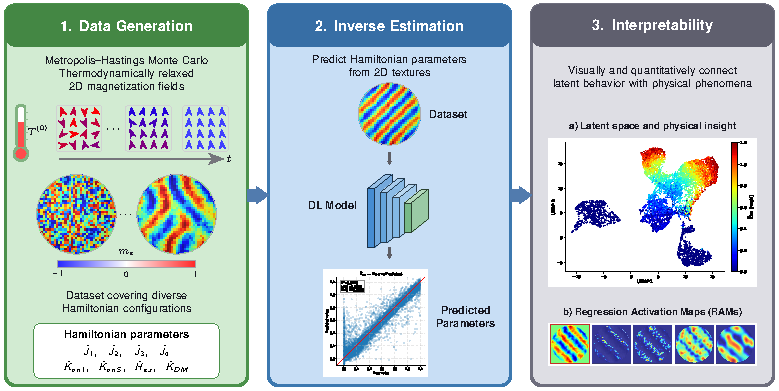
\includegraphics{graphical}}
%    \label{fig:graphical_abstract}
%\end{figure}
%\end{graphicalabstract}



%%Research highlights

%\begin{highlights}
%\item Atomistic Hamiltonian generates relaxed 2D magnetic domain images for training.
%\item Deep learning regression recovers Hamiltonian parameters from nanodot images.
%\item Regression Activation Maps explain continuous prediction errors spatially.
%\item Framework isolates degenerate textures linking black-box AI to magnetic physics.
%\end{highlights}




\begin{keyword}
Explainable AI \sep Magnetic Nanodots \sep Hamiltonian Parameters \sep Regression Activation Maps \sep Deep Learning
\end{keyword}

\end{frontmatter}

\linenumbers


\section{Introduction}\label{sec:intro}

%nanoscale motivation and structures: helical, labyrinth and skyrmion
Understanding and controlling magnetic behavior at the nanometric scale is a central challenge in modern condensed matter physics and materials engineering~\cite{heinrich2021quantum}. This capability is particularly relevant to the development of spintronic devices, ultrahigh-density magnetic memories, and neuromorphic computing platforms based on topological magnetic textures~\cite{fert2024electrical}. At such length scales, surface effects, geometric confinement, and energy quantization substantially modify magnetic properties relative to the bulk~\cite{issa2013magnetic}. The resulting enhancement of surface anisotropy, structural imperfections, and thermal fluctuations strongly affects the stability and dynamics of spin configurations~\cite{charalampidis2023metadynamics}. These effects give rise to emergent collective states—including ferromagnetic, helical, labyrinthine, and skyrmionic textures~\cite{yu2021magnetic}—whose stability is governed by the interplay of competing microscopic interactions~\cite{tokura2020magnetic}. In this context, magnetic nanodots constitute an ideal model platform, as their lateral confinement favors the formation of single-domain states, vortices, and skyrmion-like configurations controlled by the balance among symmetric exchange, magnetic anisotropy, DMI, and external magnetic fields~\cite{rohart2013skyrmion}. Therefore, inferring these underlying physical parameters directly from magnetic domain images has become a critical inverse problem for the rational engineering of functional magnetic materials~\cite{kong2023quantifying}.

%hammiltonian and ill conditioned problem (degenerecy)
Within this framework, atomistic Hamiltonian-based modeling constitutes the most rigorous description of the discrete spin interactions, localized dynamics, and boundary effects that dominate nanoscale magnetic systems. Unlike continuum micromagnetic models, which can mask essential surface and finite-size contributions, the extended Heisenberg Hamiltonian explicitly captures the atomistic interactions responsible for stabilizing complex topological textures in magnetic nanodots~\cite{evans2014atomistic}. In its general form, the Hamiltonian includes several competing terms: the symmetric exchange interaction ($\tilde{J}$ [meV]), which promotes collinear alignment; the DMI ($\tilde{K}_{DM}$ [meV]), which favors chiral and non-collinear spin textures; the magnetocrystalline anisotropy ($\tilde{K}$ [meV]), which selects preferred crystallographic orientations; and the Zeeman coupling to an external magnetic field ($\tilde{H}_{ex}$ [meV])~\cite{aldarawsheh2023intrinsic}. The competition among these contributions generates a highly multimodal energy landscape~\cite{tokura2020magnetic}, in which physically distinct parameter sets may produce spin states with nearly indistinguishable out-of-plane textures, allowing helical, skyrmion-like, and other metastable configurations to coexist~\cite{back20202020}. Compounded by the noise that external conditions and transient states introduce during thermal relaxation, this degeneracy renders the inverse estimation of Hamiltonian parameters from two-dimensional magnetic domain images intrinsically ill-conditioned, imposing a physical limit on parameter identifiability that must be explicitly characterized rather than assumed away~\cite{murakami2022inverse, kwon2020magnetic}.

% SOTA 1: Experimental and simulation limitations
The intrinsic ambiguity of the inverse problem is further exacerbated by the limitations of current experimental and analytical methodologies. Although advanced imaging techniques, including magnetic force microscopy, Lorentz transmission electron microscopy, and spin-polarized scanning tunneling microscopy~\cite{nguyen2022cooperative}, enable high-resolution visualization of magnetic textures, they typically provide indirect or transformed measurements that are subject to modality-dependent distortions, noise, and finite spatial resolution~\cite{zhao2025overview, gaida2023lorentz}. In practice, parameter estimation therefore relies heavily on empirical fitting or on comparison with synthetic magnetic configurations generated by atomistic spin simulations or continuum micromagnetic models~\cite{d2023micromagnetic, lepadatu2021micromagnetic}. Yet similarity measures defined in image space—such as mean squared error or structural similarity—are often inadequate for resolving topologically distinct states, since they primarily quantify visual resemblance rather than physical equivalence. Consequently, the optimization process remains structurally ambiguous, and substantially different Hamiltonian parameter sets may produce magnetic domain patterns that are visually indistinguishable ~\cite{yin2023computational, karnatov2025analysis}.

% SOTA 2: Deep Learning & Interpretability challenges
To circumvent the prohibitive cost of iterative simulation-based optimization, recent efforts have reformulated this inverse problem as a data-driven learning task using deep neural architectures~\cite{lee2024deep}. Although supervised regression models allow fast parameter inference, they generally impose an implicit one-to-one mapping and therefore tend to collapse the intrinsic multimodality of degenerate magnetic systems into oversmoothed point predictions~\cite{chen2024data}. Methods designed to explicitly capture this uncertainty—such as Bayesian inference, diffusion models, cycle-consistent networks, and physics-informed neural networks—offer improved representational flexibility, but often introduce substantial computational overhead and pronounced optimization stiffness~\cite{lan2022scaling, huang2023cycle, baldan2023physics}. Beyond these computational challenges, a central limitation remains their opacity. In strongly degenerate parameter spaces, conventional black-box models offer little or no mechanistic understanding of how localized spatial features contribute to the inferred Hamiltonian parameters~\cite{wang2021learning, vcadevz2026neural}. Moreover, although gradient-based attribution tools such as class activation maps are widely used in classification, analogous interpretability methods for continuous regression in highly multimodal physical systems remain underdeveloped~\cite{he2022survey}. This interpretability gap restricts the physical traceability required for robust and scientifically meaningful machine-learning-based inference.

\ch{Recent advances have demonstrated the immense potential of deep learning in resolving the inverse problem of magnetic Hamiltonian parameter estimation from domain images. For example, Kwon \textit{et al.} \cite{kwon2020magnetic} employed ResNet architectures to estimate Dzyaloshinskii-Moriya, anisotropy, and dipolar interactions from Monte Carlo-simulated spin configurations, while Kong \textit{et al.} \cite{kong2023quantifying} utilized customized convolutional neural networks to extract exchange stiffness, effective anisotropy, and interfacial DMI from micromagnetic simulations. More recently, Lee \textit{et al.} \cite{lee2024deep} demonstrated the applicability of fully connected networks for estimating interlayer and intralayer interactions in twisted van der Waals magnets. Despite their impressive predictive accuracy, these pioneering approaches predominantly treat the neural network as a ``black box.'' Specifically, while some works analyze intermediate feature maps \cite{kong2023quantifying} or perform statistical error analysis \cite{kwon2020magnetic, lee2024deep}, they lack spatially resolved attribution mechanisms to explicitly identify which morphological features of the spin textures drive specific parameter predictions. Furthermore, physical identifiability limits---such as degenerate spin configurations arising from competing symmetric interactions---are often encountered as empirical estimation errors rather than explicitly quantified boundaries. These gaps motivate the explainable, physics-grounded regression methodology developed in this work.}

% Proposal and Novelty
To address these limitations, we propose an inherently explainable framework grounded in an atomistic extended Heisenberg Hamiltonian. The proposed methodology explicitly captures the competition among symmetric exchange, DMI, magnetocrystalline anisotropy, and Zeeman coupling through Metropolis–Hastings Monte Carlo sampling and simulated annealing, enabling the generation of thermodynamically relaxed and highly accurate two-dimensional magnetization fields. These physically grounded data are subsequently integrated with a regression-based deep learning architecture for robust inverse estimation of the governing Hamiltonian parameters. The main contributions of this work are summarized as follows. First, we introduce a matrix/tensor decomposition of the extended Heisenberg Hamiltonian that recasts the atomistic energy as linear-algebra operations, enabling a GPU-accelerated Metropolis--Hastings Monte Carlo with simulated annealing that generates thermodynamically relaxed two-dimensional magnetization images far faster than traditional (Fortran-based) atomistic codes, without altering the underlying physics. Second, we propose Regression Activation Maps (RAMs), a novel error-based attribution method that extends gradient activation mapping to continuous-valued physical targets, turning the regressor into a traceable gray-box model that---together with UMAP/HDBSCAN clustering---links predictions to physically meaningful spin textures such as chiral domain walls and skyrmion cores. Third, we present a comparative study of convolutional and Vision Transformer regressors---contrasting their attention and RAM maps as well as their predictive accuracy relative to model size---and explicitly map the identifiability boundaries of the eight-parameter extended Heisenberg Hamiltonian from the $s_z$ projection, distinguishing reliably recoverable parameters from those that remain degenerate.

% Experiments & Results Summary
To assess the effectiveness of the proposed framework, extensive experiments were performed using a custom-generated dataset of simulated magnetic domain images covering a broad range of Hamiltonian parameter configurations. The obtained results indicate that the proposed method enables accurate inverse prediction of a subset of the Hamiltonian parameters---most notably the DMI and symmetric exchange---while explicitly exposing the identifiability limits of the remaining terms under the $s_z$ projection, with competitive performance across the evaluated convolutional and transformer models. Moreover, the qualitative and quantitative analyses based on RAMs indicate that the learned representations are associated with physically relevant spin topologies rather than dataset-specific noise or superficial correlations, thereby strengthening the interpretability and reliability of the proposed approach. The remainder of the paper is organized as follows. Section~\ref{sec:related} presents the related work. Section~\ref{sec:materials} details the materials and methods. Section~\ref{sec:experiments} describes the experimental setup. Section~\ref{sec:results_dis} presents and discusses the results. Finally, Section~\ref{sec:conclusions} concludes the paper and highlights future research directions.

\section{Related Work}\label{sec:related}

%Parameter Estimation in Nanoscale Magnetism
The inverse estimation of Hamiltonian parameters from magnetic domain configurations is widely recognized as a highly challenging problem due to the complex, nonlinear relationship between physical interactions and observable spin textures. From an experimental standpoint, researchers heavily rely on advanced indirect imaging techniques such as magnetic force microscopy, Lorentz transmission electron microscopy, and spin-polarized scanning tunneling microscopy~\cite{nguyen2022cooperative}. While these modalities enable high-resolution visualization of magnetic domains, they inherently capture transformed or partial projections of the underlying three-dimensional spin configurations. Because each technique is governed by distinct physical interaction principles, experimental observations are frequently contaminated by modality-specific distortions, finite spatial resolution limits, and heterogeneous noise, making direct inversion from these measurements generally infeasible~\cite{zhao2025overview, gaida2023lorentz}. 

%simulation methods
Consequently, practical parameter estimation heavily depends on empirical fitting or direct comparison with synthetic data generated through numerical simulations~\cite{zeng2022direct}. Computationally, the problem is most commonly addressed using physics-based forward simulations, specifically atomistic spin models governed by the extended Heisenberg Hamiltonian and continuum micromagnetic models~\cite{d2023micromagnetic, lepadatu2021micromagnetic, silva2024three}. However, attempting to optimize the inverse mapping by minimizing pixel-level discrepancy functions—such as Mean Squared Error or Mean Absolute Error—frequently fails to capture physically meaningful topological differences or vital spin interactions~\cite{talapatra2022understanding}. Even structural metrics like the Structural Similarity Index fall short in this regard~\cite{karnatov2025analysis}. Ultimately, because the comparison between simulated and experimental data occurs strictly in the image space rather than the parameter space, the optimization landscape becomes highly ambiguous, allowing disparate parameter configurations to yield visually identical domain patterns~\cite{yin2023computational}.

%Deep Learning Architectures for Inverse Parameter Inference
To bypass the computationally prohibitive nature of iterative simulation-based optimization, recent advances have increasingly framed the inverse problem as a data-driven mapping utilizing deep learning architectures~\cite{lee2024deep}. The most prevalent approach employs supervised regression models, including convolutional neural networks and transformer-based architectures, to approximate this mapping deterministically. While these models offer rapid inference and scalability, they inherently assume a one-to-one mapping between images and parameters. In highly degenerate magnetic systems, this assumption causes the models to collapse the intrinsic multimodality of the parameter space into a single, often smoothed, point estimate, rendering them highly sensitive to dataset bias and sim-to-real mismatch~\cite{chen2024data}. 

%Bayesian methods
To explicitly model uncertainty and capture this multimodality, probabilistic frameworks such as Bayesian inference methods, conditional variational autoencoders, and diffusion models have been introduced~\cite{zhao2023generative}. Despite their theoretical flexibility in sampling multiple plausible configurations, these generative and Bayesian approaches suffer from immense computational overhead, unstable training dynamics, and a distinct lack of explicit physical guarantees. In parallel, cycle-consistent frameworks and Physics-Informed Neural Networks attempt to constrain the solution space by enforcing coherence between forward and inverse mappings, or by directly embedding thermodynamic penalties into the loss function~\cite{huang2023cycle, baldan2023physics}. While physically plausible, these hybrid models introduce severe optimization stiffness and rely fundamentally on the accuracy of the underlying forward surrogate, which can dangerously propagate errors within strongly degenerate spin regimes.

%Explainability and Interpretability in Physical Machine Learning
Despite the growing predictive capabilities of advanced deep neural networks, their fundamental opacity remains a critical barrier to their widespread adoption in condensed matter physics. In the context of nanoscale magnetism, the delicate energetic competition among the exchange interaction, the DMI, and magnetocrystalline anisotropy creates a densely degenerate parameter space where multiple physical configurations present nearly identical free energies~\cite{vcadevz2026neural}. Traditional black-box deep learning architectures provide no mechanistic insight into how specific spatial features within a magnetic domain image correlate with the predicted Hamiltonian constants~\cite{wang2021learning}. This lack of interpretability prevents researchers from distinguishing whether a model has genuinely captured the underlying physical laws or merely memorized superficial dataset artifacts. While gradient-based attribution methods like Class Activation Maps have been widely adopted for discrete classification tasks, interpreting continuous regression outputs in highly multimodal physical systems remains largely underexplored~\cite{he2022survey}. The inability to spatially trace and quantify the sources of prediction errors restricts the scientific traceability of these models, underscoring an urgent necessity for architectures that inherently couple high predictive accuracy with transparent, physics-informed spatial interpretations.

%novelty
To overcome these limitations, our methodology departs from prior work along three concrete axes. First, whereas most existing approaches operate at the continuum micromagnetic scale, we adopt an atomistic description at the nanometric scale, grounded in a rigorous extended Heisenberg Hamiltonian that explicitly resolves the discrete spin interactions and the surface and finite-size effects governing magnetic nanodots. Second, in contrast to the predominantly black-box models used in this field---which expose no mechanism to trace how spatial features drive the inferred parameters---we introduce RAMs, an error-based attribution method that correlates localized spatial activations with the absolute prediction error of the continuous physical targets, turning the regressor into a transparent, physically traceable gray-box model. Third, rather than relying on conventional classical simulation software, we build the data-generation process from a matrix/tensor (algebraic) decomposition of the extended Hamiltonian that, coupled with GPU computing, substantially accelerates the Metropolis--Hastings Monte Carlo with simulated annealing without altering the underlying physics. Together, these choices couple physics-grounded, high-throughput simulation with an inherently explainable regression model, enabling the precise isolation of the degenerate magnetic textures---such as chiral domain walls and skyrmions---that drive specific parameter estimations, and establishing a reliable, transparent, and traceable pathway for analyzing complex nanoscale magnetic systems. Table~\ref{tab:literature_comparison} contrasts these distinctions with representative deep-learning approaches for magnetic Hamiltonian parameter estimation across six technical dimensions.

\begin{table}[H]
\centering
\caption{Comparative analysis of deep learning approaches for magnetic Hamiltonian parameter estimation. The works of Kong~\textit{et al.}~\cite{kong2023quantifying}, Kwon~\textit{et al.}~\cite{kwon2020magnetic}, and Lee~\textit{et al.}~\cite{lee2024deep} are contrasted against the proposed framework across six technical dimensions.}
\label{tab:literature_comparison}
\setlength{\tabcolsep}{3pt}
\resizebox{\columnwidth}{!}{%
\begin{tabular}{@{}p{1.35cm} p{1.55cm} p{1.5cm} p{1.5cm} p{2.1cm}@{}}
\toprule
\textbf{\scriptsize Dimension} & \textbf{\scriptsize Kong~\cite{kong2023quantifying}} & \textbf{\scriptsize Kwon~\cite{kwon2020magnetic}} & \textbf{\scriptsize Lee~\cite{lee2024deep}} & \textbf{\scriptsize Ours} \\
\midrule
\textbf{\scriptsize Hamiltonian terms}
& \scriptsize Exchange $A$, aniso.\ $K_\text{eff}$, DMI $D$
& \scriptsize Exchange $J$, DMI $\beta$, dipolar $D$, aniso.\ $K$
& \scriptsize Intralayer $J$, single-ion $A$, interlayer $J^{\perp}$
& \scriptsize Ext.\ Heisenberg $\tilde{J}_1$--$\tilde{J}_4$, $\tilde{K}_{DM}$, $\tilde{H}_{ex}$, $\tilde{K}_{an1}$, $\tilde{K}_{anS}$ \\
\midrule
\textbf{\scriptsize Simulation}
& \scriptsize Micromagnetic (mumax3, LLG)
& \scriptsize MC simulated annealing
& \scriptsize Atomistic (stochastic LLG)
& \scriptsize Atomistic MC (Metropolis + annealing, multi-GPU) \\
\midrule
\textbf{\scriptsize DL architecture}
& \scriptsize Custom CNN
& \scriptsize ResNet18/50, CNN
& \scriptsize MLPs
& \scriptsize CNN baseline + DenseNet, ViT, Xception, ResNet \\
\midrule
\textbf{\scriptsize Params.\ estimated}
& \scriptsize 4
& \scriptsize 3
& \scriptsize 3
& \scriptsize 8 \\
\midrule
\textbf{\scriptsize Metrics}
& \scriptsize MAE, $R^2$
& \scriptsize MAE, PCA of errors
& \scriptsize MAPE, MSE
& \scriptsize $R^2$, MAE + UMAP/ HDBSCAN clustering \\
\midrule
\textbf{\scriptsize Interpret.}
& \scriptsize Feature maps (black box)
& \scriptsize Black box
& \scriptsize Black box (PCA)
& \scriptsize \textbf{RAMs} (layer/ structure) + identifiability \\
\bottomrule
\end{tabular}%
}
\end{table}



\section{Materials and Methods}\label{sec:materials}

\subsection{Atomistic Hamiltonian Framework}\label{sec:hamiltonian}

%hamiltonian fundaments
The theoretical foundation for modeling interacting magnetic dipole moments originates from the seminal formulations of Ernst Ising and Werner Heisenberg~\cite{agudelo2019study}. Ising introduced a one-dimensional statistical mechanics model wherein localized spins were heavily constrained to discrete, scalar states (i.e., rigidly pointing ``up'' or ``down''). While the Ising model provided early fundamental insights into macroscopic ferromagnetism and phase transitions, its strict uni-axial constraint renders it structurally insufficient for capturing the continuous rotational degrees of freedom required to model complex, multi-dimensional magnetic textures. This limitation was subsequently resolved by Heisenberg, who formulated a generalized model allowing spin vectors to vary continuously in three-dimensional space with rotational symmetry. While the foundational 
Heisenberg model successfully captures isotropic exchange driven by the Pauli exclusion principle, modern nanoscale applications—such as the study of magnetic vortices and topologically protected skyrmions in confined nanodot geometries—necessitate an extended 
approach~\cite{fert2024electrical}. This extended framework rigorously incorporates symmetry-breaking relativistic spin-orbit coupling effects, primarily the DMI and magnetocrystalline anisotropy, alongside standard Zeeman coupling~\cite{borisov2021heisenberg}.

%generalized formulation
Formally, let $\mathcal{V} = \{1, \dots, N\}$ denote the set of indices for the discrete magnetic lattice sites. The thermodynamic state of the system is characterized by the spatial distribution of localized magnetic moments, represented by the normalized spin vectors $\mathbf{s}_i \in \mathbb{R}^3$, subject to the constraint 
$\|\mathbf{s}_i\|_2 = 1$, for $i\in\mathcal{V}$. In a generalized theoretical context, all pairwise symmetric and antisymmetric interactions, as well as site-specific field and anisotropy alignments, can be collapsed into a unified geometric approach~\cite{moriya1960anisotropic, eriksson2017atomistic}. The total effective energy of the system $\mathcal{H}\in\mathbb{R}$ [meV] is thus defined by the following generalized quadratic form:

\begin{equation}\label{eq:GeneralizedHamiltonian}
\begin{split}
\mathcal{H}\left(\mathbf{S}| \breve{\theta}\right) ={}
&- \sum_{i=1}^{N}\sum_{j\in \mathcal{N}(i)}
    \langle \mathbf{s}_i, \tilde{\mathbf{M}}_{ij}\mathbf{s}_j \rangle \\
&- \sum_{i=1}^{N} \langle\tilde{\mathbf{h}}_{i},\mathbf{s}_i\rangle
- \sum_{i=1}^{N} \langle\mathbf{s}_i \tilde{\mathbf{K}}_i,
    \mathbf{s}_i\rangle,
\end{split}
\end{equation}
where $\mathcal{N}(i)$ defines the set of interacting nearest neighbors for a given site $i$, and the matrix $\mathbf{S}\in\mathbb{R}^{N\times 3}$ 
gathers the continuous spin vectors across the lattice with 
$\mathbf{s}_i\in\mathbf{S}$. Here, 
$\breve{\theta}=\{\tilde{\mathbf{M}}_{ij},\tilde{\mathbf{h}}_{i},
\tilde{\mathbf{K}}_{i}\}$, where 
$\tilde{\mathbf{M}}_{ij} \in \mathbb{R}^{3 \times 3}$ represents the complete bilinear interaction matrix coupling neighboring spins, $\tilde{\mathbf{h}}_i \in \mathbb{R}^{3}$ accounts for linear external field interactions, and $\tilde{\mathbf{K}}_i \in \mathbb{R}^{3 \times 3}$
is the anisotropy tensor governing site-specific directional preferences. Casting every interaction as dense linear-algebra operations acting on the spin matrix $\mathbf{S}$ is a deliberate modeling choice: it recasts the atomistic energy as batched matrix and tensor products rather than the sequential site-by-site loops of conventional atomistic codes, which is precisely what enables the GPU-accelerated evaluation and sampling detailed in Section~\ref{sec:montecarlo_sim}, without altering the underlying physics.

%Decomposition and Factorization
Afterward, to recover the isolated physical phenomena and define an extended target scalar parameter space 
$\boldsymbol{\theta}=[\tilde{J}_1,\tilde{J}_2,\tilde{J}_3,\tilde{J}_4,
\tilde{K}_{DM},\tilde{H}_{ex},\tilde{K}_{an1},\tilde{K}_{anS}]$, the generalized matrices must be mathematically decomposed. By factorizing these parameters, we can map each matrix operation to its specific energetic contribution:

\begin{itemize}

    \item[--] \emph{Bilinear Coupling ($\tilde{\mathbf{M}}_{ij}$):} A 
    real square matrix can be separated into its symmetric and skew-symmetric components. Here, 
    $\tilde{\mathbf{M}}_{ij}$ is parameterized by factorizing the isotropic exchange scalar $\tilde{J}_r$ for the $r$-th neighbor shell and the DMI magnitude $\tilde{K}_{DM}$ along a predefined spatial direction vector $\hat{\mathbf{d}}_{ij} \in \mathbb{R}^3$ 
    ($\|\hat{\mathbf{d}}_{ij}\|_2=1$), yielding:
    
    \begin{equation}\label{eq:MatrixDecomposition}
    \tilde{\mathbf{M}}_{ij}(\tilde{J}_r,\tilde{K}_{DM}) = 
        \tilde{J}_r \mathbf{I} - \tilde{K}_{DM} [\hat{\mathbf{d}}_{ij}]_{\times},
    \end{equation}
    where $\mathbf{I} \in \mathbb{R}^{3 \times 3}$ represents the identity matrix and 
    $[\hat{\mathbf{d}}_{ij}]_{\times} \in \mathbb{R}^{3 \times 3}$ denotes the skew-symmetric matrix representation of the cross-product. The symmetric exchange is modeled across four neighbor shells $r \in \{1,2,3,4\}$, where $\mathcal{N}_r(i)$ denotes the 
    set of neighbors at shell $r$ around site $i$, ordered by 
    increasing interatomic distance ($d_1 < d_2 < d_3 < d_4$). To resolve the fundamental scale ambiguity of the inverse problem---whereby multiplying all parameters by a common factor leaves the observable spin configuration unchanged---the first-shell exchange is fixed as the energy reference unit, $\tilde{J}_1\in \mathbb{R}$ in meV, while $\tilde{J}_2, \tilde{J}_3, \tilde{J}_4 \in \mathbb{R}$ are free parameters (also in meV). The DMI acts exclusively between first-shell neighbors and is therefore indexed only over $\mathcal{N}_1(i)$.

    \item[--] \emph{Zeeman Interaction ($\tilde{\mathbf{h}}_i$):} The linear field term is factorized by extracting the scalar field magnitude $\tilde{H}_{ex}$ and a fixed normalized direction vector
    $\hat{\mathbf{h}}$, with
    $\|\hat{\mathbf{h}}\|_2 = 1$, of the externally applied
    magnetic field, yielding $\tilde{\mathbf{h}}_i = \tilde{H}_{ex}\,\hat{\mathbf{h}}\in\mathbb{R}^3$. The orientation $\hat{\mathbf{h}}$ is held constant within each simulation but is selected among the principal crystallographic axes---either in-plane ($\hat{\mathbf{e}}_x$) or out-of-plane ($\hat{\mathbf{e}}_z$)---to stabilize distinct families of topological textures. Fixing this direction eliminates the orientational degree of freedom of $\tilde{\mathbf{h}}_i$, ensuring that $\tilde{H}_{ex}$ alone serves as the free parameter governing the Zeeman
    contribution.

    \item[--] \emph{Magnetocrystalline Anisotropy 
    ($\tilde{\mathbf{K}}_i$):} Modeling cubic magnetocrystalline anisotropy requires factorizing a site-dependent scalar constant $\tilde{K}_i^{eff}$ to scale a quartic interaction. The principal crystallographic axes of the nanodot are defined by the orthonormal basis vectors $\mathbf{e}_{\hat{x}}, \mathbf{e}_{\hat{y}}, 
    \mathbf{e}_{\hat{z}} \in \mathbf{E}$, with $\mathbf{E} \in \mathbb{R}^{3 \times 3}$, and the directional cosines are given by $s_{im} = \langle \mathbf{e}_m,\mathbf{s}_i\rangle$ 
    ($\forall m\in\{\hat{x},\hat{y},\hat{z}\}$). Because atoms at the nanodot surface experience broken inversion symmetry---having fewer neighbors on the exterior side---their anisotropy differs fundamentally from that of interior atoms. The lattice is therefore partitioned into two disjoint subsets: the bulk region $\mathcal{V}_{bulk} \subset \mathcal{V}$, comprising interior sites with complete coordination shells, and the surface region 
    $\mathcal{V}_{surf} \subset \mathcal{V}$, comprising boundary sites exposed to the geometric confinement, with 
    $\mathcal{V}_{bulk} \cup \mathcal{V}_{surf} = \mathcal{V}$ and $\mathcal{V}_{bulk} \cap \mathcal{V}_{surf} = \emptyset$. This yields the site-dependent effective anisotropy constant:
    
    \begin{equation}\label{eq:AnisotropyEffective}
    \tilde{K}_i^{eff} = 
    \begin{cases}
        \tilde{K}_{an1} & \text{if } i \in \mathcal{V}_{bulk}, \\
        \tilde{K}_{anS} & \text{if } i \in \mathcal{V}_{surf},
    \end{cases}
    \end{equation}
    where $\tilde{K}_{an1}, \tilde{K}_{anS} \in \mathbb{R}$ are scalar constants measured in meV per atom~\cite{cullity2011introduction}.

\end{itemize}

%Explicit Formulation
Substituting these factorized relationships back into 
Equation~\ref{eq:GeneralizedHamiltonian} yields the following explicit formulation for the total extended Hamiltonian:

\begin{equation}\label{eq:Hamiltonian}
\begin{split}
\mathcal{H}\left(\mathbf{S}|\hat{\mathbf{d}}_{ij},\hat{\mathbf{h}};
\boldsymbol{\theta}\right) ={}
&- \sum_{r=1}^{4}\tilde{J}_r
    \sum_{i=1}^{N}\sum_{j\in \mathcal{N}_r(i)}
    \langle \mathbf{s}_i, \mathbf{s}_j \rangle \\
&+ \tilde{K}_{DM} \sum_{i=1}^{N}\sum_{j\in \mathcal{N}_1(i)}
    \langle \hat{\mathbf{d}}_{ij},(\mathbf{s}_i \times \mathbf{s}_j)
    \rangle \\
&- \tilde{H}_{ex} \sum_{i=1}^{N}
    \langle \hat{\mathbf{h}}, \mathbf{s}_i \rangle \\
&+ \frac{1}{S_o^4}\sum_{i=1}^{N} \tilde{K}_i^{eff}
    \left(s_{i\hat{x}}^2 s_{i\hat{y}}^2 +
          s_{i\hat{x}}^2 s_{i\hat{z}}^2 +
          s_{i\hat{y}}^2 s_{i\hat{z}}^2\right),
\end{split}
\end{equation}
with $\tilde{J}_1 = 1.0$~meV fixed as the energy reference unit. The cubic anisotropy form in the last term follows directly from expanding $\frac{1}{2}(1 - \|\mathbf{s}_i\mathbf{E}\|_4^4)$ under the $L_2$ normalization constraint $\|\mathbf{s}_i\|_2 = 1$, which 
yields $s_{i\hat{x}}^2 s_{i\hat{y}}^2 + s_{i\hat{y}}^2 
s_{i\hat{z}}^2 + s_{i\hat{z}}^2 s_{i\hat{x}}^2$, normalized by $S_o^4$ to maintain dimensional consistency across spin magnitudes.

%parameter interpretation
Physically, the extended parameter space $\boldsymbol{\theta}$ actively governs the competing energetic contributions that shape the magnetic energy landscape. Each $\tilde{J}_r$ dictates the collinear alignment tendency between spin pairs separated by the corresponding distance~\cite{coey2010magnetism}: positive values ($\tilde{J}_r > 0$) favor parallel, ferromagnetic 
alignment, while negative values ($\tilde{J}_r < 0$) drive 
antiparallel, antiferromagnetic order. This multi-shell formulation is essential in confined nanodot geometries, where longer-range exchange pathways--mediated through intermediate atomic orbitals--contribute non-negligibly to the global energetic competition and can selectively stabilize or destabilize complex topological textures beyond what first-shell interactions alone would predict~\cite{eriksson2017atomistic}. Among these constants, $\tilde{J}_1$ plays a privileged role: it 
corresponds to the strongest and most spatially direct exchange pathway, coupling each spin to its nearest neighbors in the cubic lattice and establishing the dominant energy scale of the magnetic system. For this reason, $\tilde{J}_1$ is fixed to $1.0$~meV throughout all simulations, serving as the absolute energy reference unit against which all remaining interaction strengths are expressed. The remaining constants $\tilde{J}_2$, $\tilde{J}_3$, and $\tilde{J}_4$ are free parameters whose magnitudes decay with increasing shell distance, consistent with the exponential attenuation of quantum mechanical exchange integrals with interatomic separation~\cite{coey2010magnetism}.

The DMI magnitude, represented by $\tilde{K}_{DM}$, is responsible for driving chiral, non-collinear spin winding in systems exhibiting broken spatial inversion symmetry~\cite{fert2017magnetic}. By actively competing with the dominant first-shell exchange $\tilde{J}_1$, 
this antisymmetric contribution stabilizes complex topological textures, such as chiral domain walls and skyrmions. It acts exclusively between first-shell neighbors, as longer-range antisymmetric exchange pathways are negligibly small compared to the dominant spin-orbit coupling at nearest-neighbor interfaces. Measured in meV per interacting spin pair, its magnitude is fundamentally dependent on the strength of the spin-orbit coupling
at the material's interfaces and is naturally expressed as a fraction of the first-shell exchange energy $\tilde{J}_1$~\cite{fert2017magnetic}; the specific sampled range and its physical justification are detailed in Section~\ref{sec:experiments}.

The Zeeman coupling energy, parameterized as $\tilde{H}_{ex}$, quantifies the interaction between the localized atomic spins and the externally applied magnetic field~\cite{evans2014atomistic}. It systematically 
penalizes magnetic misalignment with the fixed field axis $\hat{\mathbf{h}}$, frequently serving as the primary thermodynamic driving force for macroscopic magnetic phase transitions. This
parameter is expressed in meV per atom, mathematically representing the effective energy equivalence ($g\mu_B B$) that transitions a macroscopic magnetic field $B$ measured in Tesla into the atomistic energy regime; with $g\approx2$ this corresponds to $\approx 0.116$~meV per Tesla, so that the sampled range maps directly onto laboratory-accessible fields (Section~\ref{sec:experiments}). Also, fixing the field direction along $\hat{\mathbf{h}}$ reduces the dimensionality of the inverse problem by eliminating the orientational degree of freedom of $\tilde{\mathbf{h}}_i$, ensuring that $\tilde{H}_{ex}$ alone governs the Zeeman contribution as a single identifiable scalar. Notably, when the field is applied out-of-plane ($\hat{\mathbf{h}} = \hat{\mathbf{e}}_z$), the Zeeman term couples directly to the observable $s_z$ component, which---as discussed below---renders $\tilde{H}_{ex}$ recoverable from the two-dimensional projection.

Finally, the magnetocrystalline anisotropy encodes the intrinsic directional preference for magnetization relative to the underlying crystal lattice~\cite{cullity2011introduction}. Arising from 
relativistic spin-orbit coupling, this term rigorously establishes the energetically favorable (easy) and unfavorable (hard) crystallographic axes for spin orientation within the nanodot. Both constants are measured in meV per atom and represent a relatively subtle symmetry-breaking energy compared to the dominant isotropic 
exchange. The bulk anisotropy constant $\tilde{K}_{an1}$ governs interior lattice sites $i \in \mathcal{V}_{bulk}$, where each atom is fully coordinated by neighbors in all spatial directions, yielding a locally symmetric energetic environment. Its magnitude ranges from near-zero in soft magnets to several meV per atom in strongly anisotropic interfacial systems~\cite{cullity2011introduction, gambardella2003giant}, with the sampled range specified in Section~\ref{sec:experiments}. The surface anisotropy constant $\tilde{K}_{anS}$, by contrast, 
governs boundary sites $i \in \mathcal{V}_{surf}$, where broken spatial inversion symmetry---arising from the absence of neighbors on the exterior side of the nanodot---produces an asymmetric local environment that intensifies the directional preference for spin orientation. Consequently, $|\tilde{K}_{anS}|$ is generally larger than $|\tilde{K}_{an1}|$, reflecting the enhanced symmetry-breaking at the nanodot boundary. This two-constant formulation is essential for accurately capturing the finite-size and surface-dominated effects that critically govern the stability of emergent topological textures
in confined nanoscale geometries~\cite{fert2024electrical, borisov2021heisenberg}.

Although the parameter vector $\boldsymbol{\theta}$ governs the full three-dimensional spin field, the observable exploited in this work is restricted to its out-of-plane projection, the $s_z$ component. This choice is dictated by experimental measurability: the most widely available magnetic imaging modalities---such as magnetic force microscopy and the polar magneto-optical Kerr effect---are primarily sensitive to the out-of-plane magnetization~\cite{li2023magnetic}, whereas resolving the in-plane components requires substantially more specialized techniques. Working on $s_z$ therefore keeps the framework consistent with the information realistically accessible from experiment. This restriction, however, imposes a theoretical limit on parameter identifiability: distinct parameter sets---most notably those related by the sign of the antisymmetric exchange, which reverses the in-plane chirality while leaving $s_z$ invariant---become indistinguishable in the observation space, so that a regressor exposed to both would collapse its predictions toward a degenerate average. To avoid this pathology, the present study deliberately samples the Hamiltonian parameters over value ranges that remain well-posed under the $s_z$-only observation, ensuring that the retained configurations do not induce the aforementioned averaging saturation; the specific bounds and the associated sign convention are detailed in Section~\ref{sec:experiments}.

\subsection{Image-Based Dataset Generation From Monte Carlo Simulations}\label{sec:montecarlo_sim}

To accurately capture the physical thermodynamic behavior and algorithmically \ch{drive the system toward a low-energy, thermodynamically stable configuration} of the nanodot, thermal fluctuations must be formally introduced through the framework of statistical mechanics. While the atomistic Hamiltonian $\mathcal{H}$ rigorously defines the internal magnetic energy for a given spatial configuration of spins, it evaluates the system strictly as a frozen, zero-temperature snapshot. Hence, temperature is fundamentally a macroscopic parameter that governs the statistical distribution of the discrete magnetic microstates rather than acting as a localized interaction within the Hamiltonian. Consequently, temperature $T$ $[K]$ couples to the system via the Boltzmann distribution~\cite{eriksson2017atomistic}. Formally, a magnetic microstate $\mu$ represents a specific, instantaneous realization of the continuous spin matrix, denoted as $\mathbf{S}_\mu$. The total thermodynamic energy of this specific configuration is evaluated against the static environmental vectors and physical interaction strengths, such that $\mathcal{H}(\mu) \equiv \mathcal{H}\left(\mathbf{S}_\mu|\mathbf{\hat{d}}_{ij},\hat{\mathbf{h}},\mathbf{E};\boldsymbol{\theta}\right)$. At thermal equilibrium, the probability $P(\mu)$ of the system occupying this specific microstate is defined as:

\begin{equation}\label{eq:Boltzmann}
P(\mu) = \frac{1}{\mathcal{Z}} \exp\left(-\frac{\mathcal{H}(\mu)}{k_B T}\right),
\end{equation}
where $k_B$ is the Boltzmann constant (expressed in $\text{meV/K}$). The term $\mathcal{Z}$ represents the canonical partition function, which mathematically enforces probability normalization by summing over all valid spin configurations $\nu$ (i.e., all possible state matrices $\mathbf{S}_\nu$ strictly satisfying the geometric boundary constraint $\|\mathbf{s}_i\|_2 = 1$):

\begin{equation}\label{eq:PartitionFunction}
\mathcal{Z} = \sum_{\mathbf{S}_\nu} \exp\left(-\frac{\mathcal{H}\left(\mathbf{S}_\nu|\mathbf{\hat{d}}_{ij},\hat{\mathbf{h}},\mathbf{E};\boldsymbol{\theta}\right)}{k_B T}\right).
\end{equation}

In our computational framework, this thermodynamic distribution is actively sampled using the Metropolis-Hastings Monte Carlo algorithm combined with a simulated annealing protocol~\cite{landau2021guide}. This stochastic sampling ensures a rigorous exploration of the highly multimodal energy landscape characteristic of these degenerate magnetic systems. When a localized spin perturbation proposes a physical transition from the current microstate $\mu^{(t)}$ (characterized by $\mathbf{S}_{\mu^{(t)}}$) to a newly modified state $\mu^{(t+1)}$ (characterized by $\mathbf{S}_{\mu^{(t+1)}}$), the resulting change in the system's total energy is computed as the scalar difference $\Delta \mathcal{H} = \mathcal{H}(\mu^{(t+1)}) - \mathcal{H}(\mu^{(t)})$. To optimize computational efficiency, $\Delta \mathcal{H}$ is evaluated locally at the perturbed lattice site. The proposed state is subsequently accepted or rejected based on the precise transition probability:

\begin{equation}\label{eq:Metropolis}
P(\mu^{(t)} \rightarrow \mu^{(t+1)}) = \begin{cases}
1 & \text{if } \Delta \mathcal{H} < 0 \\
\exp\left(-\frac{\Delta \mathcal{H}}{k_B T^{(t)}}\right) & \text{if } \Delta \mathcal{H} \geq 0.
\end{cases}
\end{equation}

Physically, the instantaneous temperature parameter $T^{(t)}$ actively scales the energetic barriers within the system's vast topological energy landscape during the annealing process~\cite{landau2021guide}. At elevated temperatures, the available thermal energy $k_B T^{(t)}$ frequently exceeds local energy penalties ($\Delta \mathcal{H}$), allowing the simulation to accept thermodynamically unfavorable spin alignments. This thermal noise provides the critical kinetic mechanism required to break out of metastable, localized energy minima, such as misaligned ferromagnetic domains~\cite{desplat2018thermal}. As $T^{(t)}$ is systematically scaled down during the annealing procedure, the probability of accepting higher-energy configurations undergoes exponential decay. \ch{This controlled thermal relaxation drives the continuous spin vector field toward a low-energy, thermodynamically stable configuration consistent with the annealing schedule, promoting the stabilization of complex chiral skyrmion textures driven by the underlying DMI. We note that while simulated annealing with a finite cooling rate does not formally guarantee convergence to the absolute global minimum---particularly in DMI-driven systems where numerous metastable chiral states may coexist---the monotonic energy decrease observed across all simulated configurations (see Section~\ref{sec:results_dis}) provides empirical evidence of thorough thermodynamic relaxation within the sampled parameter space.}

Moreover, to ensure that each simulation consistently originates from a fully randomized paramagnetic phase regardless of the specific parameter configuration, the initial annealing temperature (i.e., $T^{(t)}$ at $t=0$) is established as an \textit{exchange-normalized initial temperature}. Consistent with foundational statistical mechanics~\cite{eriksson2017atomistic}, this starting temperature is dynamically rescaled in direct proportion to the dominant symmetric exchange energy ($\tilde{J}$). This energetic normalization guarantees that the initial thermal fluctuations are strictly sufficient to overcome the highest localized energetic barriers ($\Delta \mathcal{H}$) for that specific Hamiltonian. This effectively erases initial state bias and prevents the continuous spin vector field from prematurely collapsing into metastable local minima before the controlled cooling protocol begins.

The stochastic sampling described above is realized as a fully vectorized, GPU-resident computation, which constitutes one of the core methodological contributions of this work. Leveraging the matrix formulation of Section~\ref{sec:hamiltonian}, the local energy variation $\Delta\mathcal{H}$ is not evaluated site by site---as in conventional atomistic simulators---but for the entire spin lattice at once: the neighbor contributions are gathered through tensor-shift operations and combined as batched matrix and tensor products in a single pass. To update many spins simultaneously while preserving the validity of the Markov chain, the lattice is split into two interpenetrating sublattices via a checkerboard decomposition ($(x+y+z)\bmod 2$), so that all mutually non-adjacent sites of a given sublattice are proposed and accepted in parallel within each Metropolis substep. To obtain reliable thermodynamic averages, a large ensemble of independent stochastic replicas is propagated concurrently as an additional batch dimension, and the complete annealing trajectory---both thermalization and measurement sweeps---is just-in-time compiled and executed entirely on-device, eliminating host--device transfers at every sweep. Finally, the independent parameter configurations are distributed across multiple GPUs following a single-program multiple-data scheme, so that entire families of nanodot simulations are relaxed simultaneously. This matrix-based, massively parallel formulation reduces the wall-clock cost of dataset generation by orders of magnitude relative to sequential atomistic codes, without introducing any approximation to the underlying physics.

To generate a robust and diverse dataset for deep learning evaluation, the magnetic parameters governing the Hamiltonian were systematically varied across the simulations. Key variables included the exchange interaction constant ($\tilde{J}$), the magnetocrystalline anisotropy ($\tilde{K}$), the external Zeeman field ($\tilde{H}_{ex}$), and the DMI strength ($\tilde{K}_{DM}$), alongside variations in the base initial temperature ($T^{(0)}$). Subsequently, the transformation of these raw, converged 3D spin states into normalized 2D image arrays followed a strict procedural pipeline:

\begin{itemize}
    \item[--] \emph{Geometry parsing:} Spatial coordinates defining the nanodot geometry (with a fixed disk radius and thickness as Magnetic Unit Cell (MUC) measure) were established using a binary circular lattice mask.
    \item[--] \emph{Spin state mapping:} The topological structure was projected into two dimensions by extracting the out-of-plane $s_z$ component of the continuous spin vectors ($\mathbf{s}_i$) across the valid lattice coordinates. 
    \item[--] \emph{Image rendering:} The isolated configurations were rasterized onto a fixed $\breve{H} \times \breve{W}$ pixel grid. A divergent red--blue colormap was utilized to strictly encode opposite spin polarities, visually capturing the chiral winding from the nanodot's core to its perimeter.
    \item[--] \emph{Preprocessing:} Pixel intensities corresponding to the $s_z$ magnitude were normalized to a strict interval $[0, 1]$ to ensure stable gradient flows during the deep learning optimization phase. Since every component of the target vector $\boldsymbol{\theta}$ is a scalar magnitude that remains invariant under the discrete rotational symmetries of the lattice, the dataset is stored in its raw form and augmented on the fly at training time through random $90^\circ$ rotations (Section~\ref{sec:Deep_Learning}); being proper rotations, these operations enlarge the effective sample diversity while strictly preserving both the physical parameters and the chiral handedness dictated by the DMI.
\end{itemize}

%dataset
Lastly, the simulation pipeline yields a comprehensive image-based dataset, formalized as $\mathcal{D} = \{\mathbf{X}_n, \boldsymbol{\theta}_n\}_{n=1}^{\breve{N}}$, which serves as the final collection of input-output pairs for the deep learning parameter estimation task. Each input tensor $\mathbf{X}_n \in [0,1]^{\breve{H} \times \breve{W}}$ encodes the two-dimensional spatial magnetization field (the normalized $s_z$ projection), while the corresponding target vector $\boldsymbol{\theta}_n \in \mathbb{R}^{\breve{P}}$ stores the $\breve{P}$-dimensional array of generating thermodynamic and Hamiltonian parameters (e.g., $\boldsymbol{\theta}_n = [T^{(0)}_n,\tilde{J}_{1,n},\tilde{J}_{2,n},\tilde{J}_{3,n},\tilde{J}_{4,n},\tilde{K}_{DM,n},\tilde{H}_{ex,n},\tilde{K}_{an1,n},\tilde{K}_{anS,n}]$). Figure~\ref{fig:methodology_flowchart} depicts the main flowchart of our image-based magnetic dataset generation approach.

\begin{figure*}[!t]
    \centering
    \resizebox{\linewidth}{!}{
    
    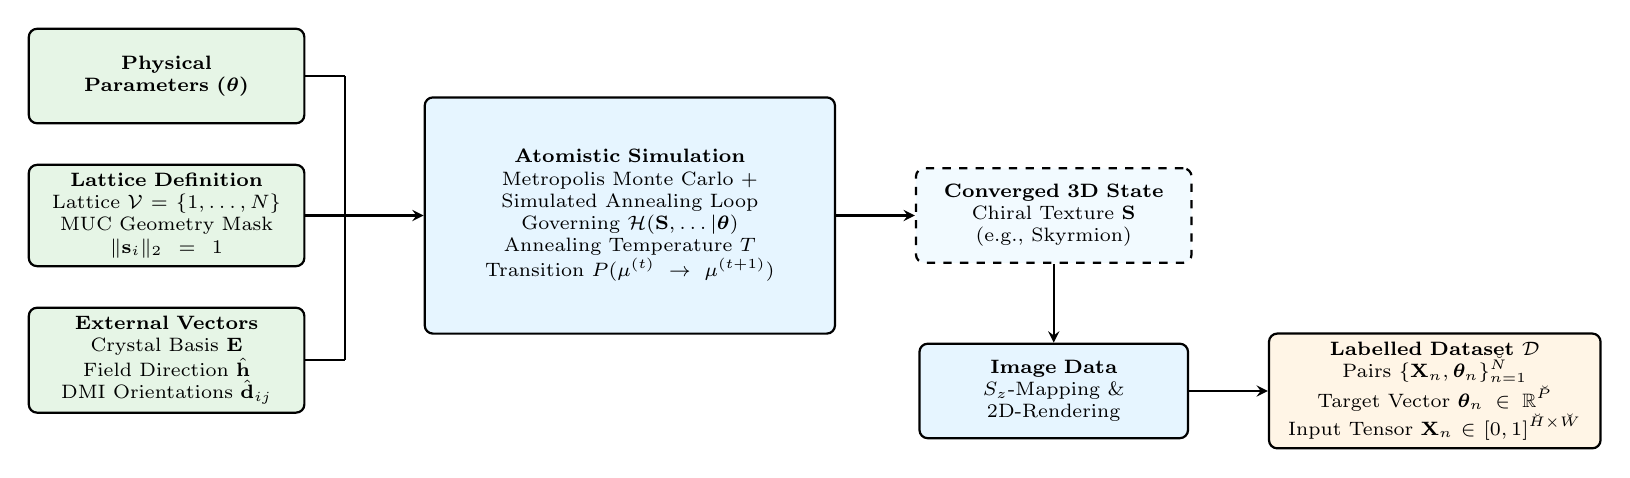
\begin{tikzpicture}[
        % --- TikZ Styles ---
        basebox/.style={
            draw, thick, minimum width=3.5cm, minimum height=1.2cm, 
            text width=3.2cm, align=center, font=\scriptsize, rounded corners=3pt,
            inner sep=3pt
        },
        inputbox/.style={basebox, fill=inputgreen},
        processbox/.style={basebox, fill=processblue},
        outputbox/.style={basebox, fill=outputorange},
        arrow/.style={thick, ->, >=stealth}
    ]

    % --- 1. INPUTS ---
    \node[inputbox] (params) {
        \textbf{Physical\\ Parameters ($\boldsymbol{\theta}$)}        
    };

    \node[inputbox, below=0.5cm of params] (lattice) {
        \textbf{Lattice Definition} \\
        Lattice $\mathcal{V}=\{1, \dots, N\}$ \\
        MUC Geometry Mask \\
        $\|\mathbf{s}_i\|_2 = 1$
    };

    \node[inputbox, below=0.5cm of lattice] (vectors) {
        \textbf{External Vectors} \\
        Crystal Basis $\mathbf{E}$ \\
        Field Direction $\hat{\mathbf{h}}$ \\
        DMI Orientations $\hat{\mathbf{d}}_{ij}$
    };

    % --- 2. SIMULATION ---
    \node[processbox, right=1.5cm of lattice, minimum height=3cm, text width=5cm] (mcsim) {
        \textbf{Atomistic Simulation} \\
        Metropolis Monte Carlo + Simulated Annealing Loop\\
        Governing $\mathcal{H}(\mathbf{S}, \dots | \boldsymbol{\theta})$ \\
        Annealing Temperature $T$\\
        Transition $P(\mu^{(t)} \to \mu^{(t+1)})$ 
    };

    \node[processbox, fill=processblue!50, dashed, right=1cm of mcsim] (topology) {
        \textbf{Converged 3D State} \\
        Chiral Texture $\mathbf{S}$\\
        (e.g., Skyrmion)
    };

    % --- 3. DATA GENERATION ---
    \node[processbox, below=1cm of topology,minimum width=3cm] (pipeline) {\textbf{Image Data}\\
    $S_z$-{Mapping} $\&$ 2D-Rendering
    };

    \node[outputbox, right=1cm of pipeline, minimum width=4.2cm, text width=4cm] (dataset) {
        \textbf{Labelled Dataset $\mathcal{D}$} \\
        Pairs $\{\mathbf{X}_n, \boldsymbol{\theta}_n\}_{n=1}^{\breve{N}}$ \\
        Target Vector $\boldsymbol{\theta}_n \in \mathbb{R}^{\breve{P}}$\\
        Input Tensor $\mathbf{X}_n \in [0,1]^{\breve{H} \times \breve{W}}$
    };

% --- CONNECTIONS ---
    
    % 1. Inputs to Simulation (Grouped 'Bus' Routing)
    % Draw horizontal lines out from top and bottom nodes
    \draw[thick] (params.east) -- ++(0.5,0) coordinate (bus_top);
    \draw[thick] (vectors.east) -- ++(0.5,0) coordinate (bus_bot);
    
    % Connect them with a vertical line
    \draw[thick] (bus_top) -- (bus_bot);
    
    % Draw the main arrow from the center node (intersecting the bus) to the simulation
    \draw[arrow] (lattice.east) -- (mcsim.west);
    
    % 2. Simulation to Pipeline to Output
    \draw[arrow] (mcsim.east) -- (topology.west);
    \draw[arrow] (topology.south) -- (pipeline.north);
    \draw[arrow] (pipeline.east) -- (dataset.west);

    \end{tikzpicture}}
 \caption{Flowchart of the image-based magnetic dataset generation. Foundational inputs (green)---the Hamiltonian parameters $\boldsymbol{\theta}$, the unit-cell geometry, and the external directional vectors---drive the atomistic Metropolis Monte Carlo simulation with simulated annealing (blue), which relaxes the system into a converged 3D topological state. The resulting vector field is then projected, rendered, and preprocessed (yellow) into the labelled dataset $\mathcal{D}$ mapping 2D $s_z$ images to their generating parameters.}
    \label{fig:methodology_flowchart}
\end{figure*}

\subsection{Deep Regression Framework for Hamiltonian Parameter Estimation}\label{sec:Deep_Learning}

The inverse estimation of the Hamiltonian parameters and thermodynamic state from magnetic domain images is formalized as a continuous mapping problem. Given the generated dataset $\mathcal{D}$, where $\mathbf{X}_n$ represents the normalized $s_z$ spatial magnetization field and $\boldsymbol{\theta}_n$ represents the vector of generating physical parameters, we aim to learn a parameterized non-linear mapping function $f_\Theta : \mathbb{R}^{\breve{H} \times \breve{W}} \rightarrow \mathbb{R}^{\breve{P}}$, to find the predicted parameters $\hat{\boldsymbol{\theta}}_n\in\mathbb{R}^{\breve{P}}.$

Here, $f_\Theta$ denotes a deep neural network architecture parameterized by a set of learnable weights and biases $\Theta$. The optimal parameter set $\hat{\Theta}$ is obtained by minimizing a continuous loss function over the training distribution~\cite{murphy2023probabilistic}:

\begin{equation}\label{eq:LossFunction}
\hat{\Theta} = \arg\min_{\Theta} \frac{1}{\breve{N}} \sum_{n=1}^{\breve{N}} \mathcal{L}\left(\boldsymbol{\theta}_n, f_\Theta(\mathbf{X}_n)\right),
\end{equation}
where $\mathcal{L}$ represents the chosen regression objective, typically the Mean Squared Error (MSE) or Huber loss, which mitigates the influence of outlier topological states during optimization. By minimizing this objective, the network intrinsically learns to untangle the highly multimodal spatial features mapping to the specific energetic balances of the extended Heisenberg Hamiltonian.

To achieve robust feature extraction across varying scales of magnetic textures (e.g., from localized domain walls to global skyrmion geometries), this framework evaluates a conventional convolutional baseline alongside four state-of-the-art deep learning architectures: ResNet50, DenseNet, Xception, and the Visual Transformer (ViT). All models are trained from scratch on the magnetic dataset, without any transfer learning from natural-image collections. The four convolutional backbones (the baseline CNN, ResNet50, DenseNet, and Xception) share the common pipeline illustrated in Figure~\ref{fig:cnn_implementation}---a convolutional feature extractor followed by global average pooling and the regression head---and differ only in the internal structure of their convolutional block, formalized in the equations below. The ViT departs from this scheme, replacing convolutions with self-attention over image patches (Figure~\ref{fig:vit_implementation}).

\begin{itemize}

\item[--] \emph{Conventional CNN (baseline)}: To quantify the accuracy attainable without transfer learning or the specialized inductive biases of the architectures below, we include a compact convolutional network trained from scratch directly on the native-resolution $s_z$ maps. It stacks four convolutional stages of increasing width (each comprising two $3 \times 3$ convolutions with batch normalization, ReLU activation, and spatial dropout, interleaved with spatial max-pooling), followed by global average pooling and the shared regression head. Lacking residual, dense, depthwise-separable, or attention mechanisms, this baseline isolates the marginal contribution of those components to the inverse estimation and serves as the reference against which the deeper architectures are compared (see Figure~\ref{fig:cnn_implementation}).

%CNN baseline
\begin{figure*}[!t]
    \centering
    \resizebox{\linewidth}{!}{
    
    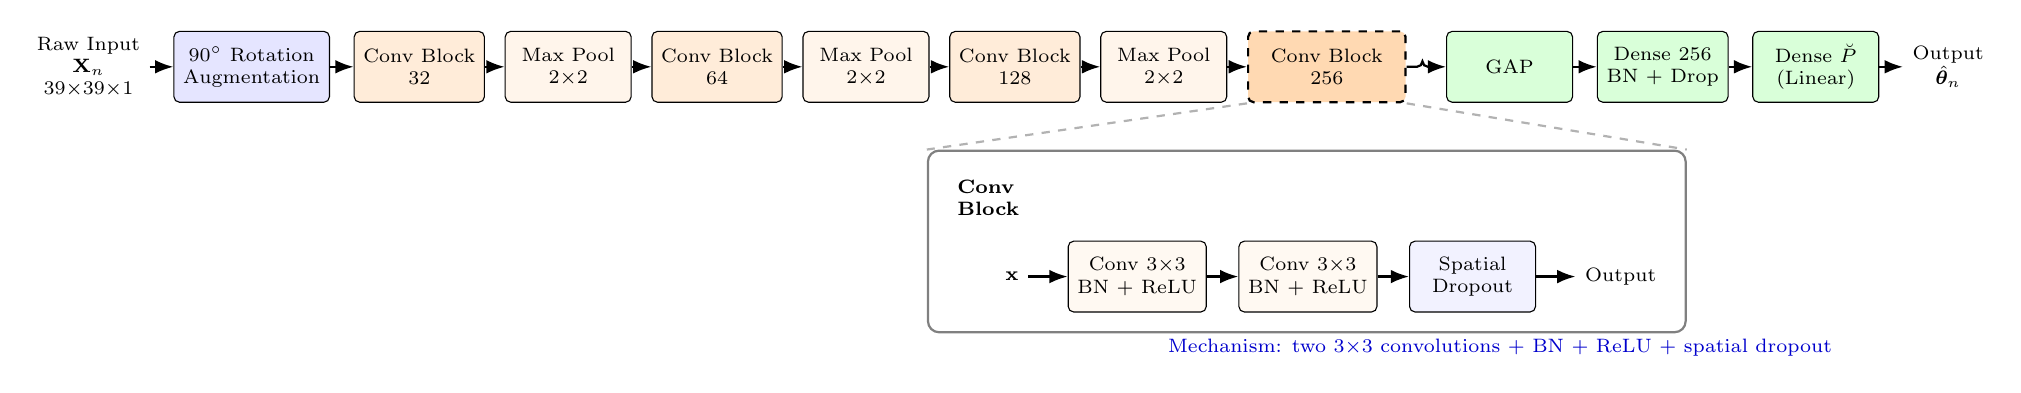
\begin{tikzpicture}[
        % Define styles for the nodes
        base_node/.style={rectangle, draw=black, minimum width=1.6cm, minimum height=0.9cm, align=center, font=\scriptsize, rounded corners=2pt},
        proc_node/.style={base_node, fill=blue!10},
        layer_node/.style={base_node, fill=orange!15},
        special_node/.style={base_node, fill=orange!30, dashed, thick, minimum width=2.0cm},
        head_node/.style={base_node, fill=green!15},
        output_node/.style={rectangle, align=center, font=\scriptsize},
        % Styles for arrows
        arrow/.style={-Latex, thick},
        skip/.style={->, thick, dashed, gray}
    ]

    % =========================================================================
    % MAIN FLOW - INPUT & AUGMENTATION (Horizontal)
    % =========================================================================
    \node (raw_input) [output_node] {Raw Input\\$\mathbf{X}_n$\\$39{\times}39{\times}1$};

    \node (aug) [proc_node, right=0.3cm of raw_input] {$90^\circ$ Rotation\\Augmentation};
    \draw [arrow] (raw_input) -- (aug);

    % =========================================================================
    % MAIN FLOW - CONVOLUTIONAL BACKBONE (Horizontal)
    % =========================================================================
    \node (cb1) [layer_node, right=0.3cm of aug] {Conv Block\\$32$};
    \draw [arrow] (aug) -- (cb1);

    \node (p1) [proc_node, fill=orange!8, right=0.25cm of cb1] {Max Pool\\$2{\times}2$};
    \draw [arrow] (cb1) -- (p1);

    \node (cb2) [layer_node, right=0.25cm of p1] {Conv Block\\$64$};
    \draw [arrow] (p1) -- (cb2);

    \node (p2) [proc_node, fill=orange!8, right=0.25cm of cb2] {Max Pool\\$2{\times}2$};
    \draw [arrow] (cb2) -- (p2);

    \node (cb3) [layer_node, right=0.25cm of p2] {Conv Block\\$128$};
    \draw [arrow] (p2) -- (cb3);

    \node (p3) [proc_node, fill=orange!8, right=0.25cm of cb3] {Max Pool\\$2{\times}2$};
    \draw [arrow] (cb3) -- (p3);

    \node (cb4) [special_node, right=0.25cm of p3] {Conv Block\\$256$};
    \draw [arrow] (p3) -- (cb4);

    % =========================================================================
    % MAIN FLOW - REGRESSION HEAD & OUTPUT (Horizontal)
    % =========================================================================
    \node (gap) [head_node, right=0.5cm of cb4] {GAP};
    \draw [arrow, rounded corners=2pt] (cb4.east) -- ++(0.2,0) |- (gap.west);

    \node (dense1) [head_node, right=0.3cm of gap] {Dense $256$\\BN $+$ Drop};
    \draw [arrow] (gap) -- (dense1);

    \node (dense2) [head_node, right=0.3cm of dense1] {Dense $\breve{P}$\\(Linear)};
    \draw [arrow] (dense1) -- (dense2);

    \node (final_output) [output_node, right=0.3cm of dense2] {Output\\$\hat{\boldsymbol{\theta}}_n$};
    \draw [arrow] (dense2) -- (final_output);

    % =========================================================================
    % INSET - CONVOLUTIONAL BLOCK DETAIL (Horizontal)
    % =========================================================================
    \begin{scope}[shift={($(cb4.south)+(-4cm, -2.2cm)$)}]

        \node[align=left, font=\scriptsize\bfseries] (inset_title) at (-0.3, 1.0) {Conv\\Block};

        \node (in_x) [output_node] at (0, 0) {$\mathbf{x}$};

        \node (c1) [proc_node, fill=orange!5, right=0.5cm of in_x] {Conv $3{\times}3$\\BN $+$ ReLU};
        \draw [arrow] (in_x) -- (c1);

        \node (c2) [proc_node, fill=orange!5, right=0.4cm of c1] {Conv $3{\times}3$\\BN $+$ ReLU};
        \draw [arrow] (c1) -- (c2);

        \node (sd) [proc_node, fill=blue!5, right=0.4cm of c2] {Spatial\\Dropout};
        \draw [arrow] (c2) -- (sd);

        \node (out_y) [output_node, right=0.5cm of sd] {Output};
        \draw [arrow] (sd) -- (out_y);

        % Math label inside inset
        \node[align=right, font=\scriptsize, blue!80!black] at (6.2, -0.9)
            {Mechanism: two $3{\times}3$ convolutions $+$ BN $+$ ReLU $+$ spatial dropout};

        % Draw Frame around inset
        \node[draw=gray, thick, fit=(inset_title) (in_x) (out_y) (sd), inner sep=0.25cm, rounded corners] (inset_frame) {};
    \end{scope}

    % Dynamic Dashed lines connecting the Backbone to the Inset
    \draw[gray!60, dashed, thick] (cb4.south west) -- (inset_frame.north west);
    \draw[gray!60, dashed, thick] (cb4.south east) -- (inset_frame.north east);

    \end{tikzpicture}
}
\caption{Shared convolutional pipeline used by all four convolutional backbones (baseline CNN, ResNet50, DenseNet, Xception): on-the-fly $90^\circ$ rotation augmentation, a convolutional feature extractor with spatial max-pooling, Global Average Pooling (GAP), and the regression head. The architectures differ only in the internal convolutional block; the inset shows the baseline block (two $3\times3$ convolutions with batch normalization, ReLU, and spatial dropout), while the residual, dense, and depthwise-separable variants are formalized in Eqs.~\ref{eq:ResNet}--\ref{eq:Xception}.}
\label{fig:cnn_implementation}
\end{figure*}

\item[--] \emph{Residual Networks (ResNet50)}~\cite{koonce2021resnet}: Standard deep convolutional networks often suffer from the vanishing gradient problem as depth increases, hindering the learning of complex physical mappings. ResNet50 circumvents this by introducing shortcut connections that bypass multiple convolutional layers, directly propagating spatial information and gradients. Mathematically, if $\mathbf{x}$ is the input to a sequence of layers, and $\mathcal{F}(\mathbf{x}, \{\mathbf{W}_l\})$ represents the residual mapping to be learned (comprising convolutions, batch normalization, and ReLU activations) for the $l$-th layer, the output $\mathbf{y}$ of the residual block is defined as:

\begin{equation}\label{eq:ResNet}
\mathbf{y} = \mathcal{F}(\mathbf{x}, \{\mathbf{W}_l\}) + \mathbf{x}.
\end{equation}

In the context of magnetic domain images, these skip connections allow the network to simultaneously preserve low-level spatial features (like abrupt chiral boundaries) while composing deep, high-level abstractions of the global thermodynamic state.

\item[--] \emph{Densely Connected Convolutional Networks (DenseNet)}~\cite{huang2017densely}: While ResNet adds features via summation, DenseNet concatenates them, maximizing information flow and feature reuse throughout the network. This is particularly advantageous for the Hamiltonian inverse problem, as the delicate energetic competition often manifests in subtle, overlapping spatial frequencies that require dense multi-scale analysis. In a DenseNet block, the feature maps of all preceding layers are used as inputs to the current layer. If $\mathbf{x}_l$ denotes the output of the $l$-th layer, and $H_l(\cdot)$ represents a composite function of batch normalization, ReLU, and convolution, the forward pass is expressed as:

\begin{equation}\label{eq:DenseNet}
\mathbf{x}_l = H_l([\mathbf{x}_0, \mathbf{x}_1, \dots, \mathbf{x}_{l-1}]),
\end{equation}
where $[\dots]$ denotes the concatenation operation. This dense topological structure ensures that the final regression head has direct access to both fine-grained pixel interactions and coarse global structures.

\item[--] \emph{Xception (Extreme Inception)}~\cite{chollet2017xception}: This architecture operates on the hypothesis that cross-channel correlations and spatial correlations in feature maps can be entirely decoupled. It replaces standard Inception modules with depthwise separable convolutions, drastically reducing computational overhead while enhancing representational efficiency. A depthwise separable convolution splits the standard convolution into two distinct steps. First, a depthwise convolution applies a single spatial filter to each input channel independently. Second, a pointwise convolution ($1 \times 1$ convolution) projects the output of the depthwise step onto a new channel space to capture cross-channel correlations. If $\mathbf{X} \in \mathbb{R}^{\breve{H} \times \breve{W} \times \breve{C}}$ is the input tensor, the operation is formally approximated as:

\begin{equation}\label{eq:Xception}
\text{Conv}_{\text{sep}}(\mathbf{X}) = \text{Conv}_{\text{pointwise}}(\text{Conv}_{\text{depthwise}}(\mathbf{X})).
\end{equation}

For nanoscale magnetism, this extreme decoupling allows the network to efficiently isolate specific topological frequency patterns (depthwise) before correlating them to the complex parameter space $\boldsymbol{\theta}_n$.



\item[--] \emph{Visual Transformer (ViT)}~\cite{dosovitskiy2020image}: Unlike Convolutional Neural Networks, which enforce a strict local inductive bias, the Vision Transformer processes the 2D spatial magnetization field $\mathbf{X}_n$ as a sequence of flattened, non-overlapping 2D patches. This allows the model to capture long-range, global dependencies across the nanodot instantly, which is critical for understanding macro-scale topological stability dictated by the Zeeman field or global anisotropy. The input image is divided into $N_p$ patches, which are linearly projected into a sequence of $D$-dimensional embeddings. The core mechanism is the Multi-Head Self-Attention (MSA), which computes attention scores to weigh the importance of different patches relative to one another. For a given set of queries $Q$, keys $K$, and values $V$ derived from the patch embeddings, the scaled dot-product attention is defined as:

\begin{equation}\label{eq:ViT}
\text{Attention}(Q, K, V) = \text{softmax}\left(\frac{QK^\top}{\sqrt{d_k}}\right)V,
\end{equation}
where $d_k$ is the scaling factor (the dimension of the keys). By employing MSA, the ViT can explicitly correlate a localized structural defect on one edge of the nanodot with a compensatory chiral boundary on the opposite edge, mapping these distant correlations directly to the global DMI or symmetric exchange strengths (see Figure~\ref{fig:vit_implementation}).

\begin{figure*}[!t]
    \centering
    \resizebox{\linewidth}{!}{
    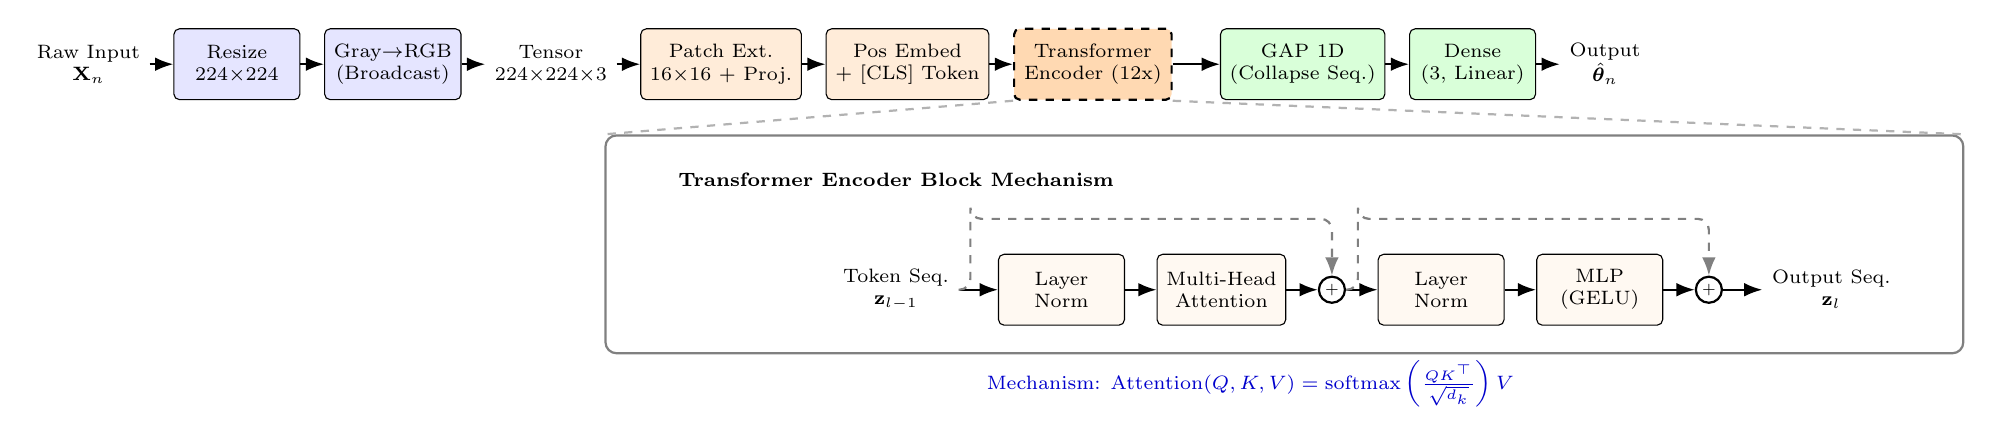
\begin{tikzpicture}[
    % Define styles for the nodes
    base_node/.style={rectangle, draw=black, minimum width=1.6cm, minimum height=0.9cm, align=center, font=\scriptsize, rounded corners=2pt},
    proc_node/.style={base_node, fill=blue!10},
    layer_node/.style={base_node, fill=orange!15},
    special_node/.style={base_node, fill=orange!30, dashed, thick, minimum width=2.0cm},
    head_node/.style={base_node, fill=green!15},
    output_node/.style={rectangle, align=center, font=\scriptsize},
    add_node/.style={circle, draw, thick, inner sep=1pt, font=\tiny},
    % Styles for arrows
    arrow/.style={-Latex, thick},
    skip/.style={-Latex, thick, dashed, gray}
]

    % =========================================================================
    % MAIN FLOW - INPUT & PREPROCESSING (Horizontal)
    % =========================================================================
    \node (raw_input) [output_node] {Raw Input\\$\mathbf{X}_n$};
    
    \node (resize) [proc_node, right=0.3cm of raw_input] {Resize\\$224{\times}224$};
    \draw [arrow] (raw_input) -- (resize);
    
    \node (rgb_map) [proc_node, right=0.3cm of resize] {Gray$\to$RGB\\(Broadcast)};
    \draw [arrow] (resize) -- (rgb_map);
    
    \node (proc_tensor) [output_node, right=0.3cm of rgb_map] {Tensor\\$224{\times}224{\times}3$};
    \draw [arrow] (rgb_map) -- (proc_tensor);

    % =========================================================================
    % MAIN FLOW - VISION TRANSFORMER BACKBONE (Horizontal)
    % =========================================================================
    \node (patching) [layer_node, right=0.3cm of proc_tensor] {Patch Ext.\\$16{\times}16$ + Proj.};
    \draw [arrow] (proc_tensor) -- (patching);
    
    \node (pos_embed) [layer_node, right=0.3cm of patching] {Pos Embed\\+ [CLS] Token};
    \draw [arrow] (patching) -- (pos_embed);

    % Highlight the Transformer Blocks as the special node linking to the inset
    \node (transformer) [special_node, right=0.3cm of pos_embed] {Transformer\\Encoder (12x)};
    \draw [arrow] (pos_embed) -- (transformer);

    % =========================================================================
    % MAIN FLOW - REGRESSION HEAD & OUTPUT (Horizontal)
    % =========================================================================
    % Using GAP1D as per the specific code implementation
    \node (gap1d) [head_node, right=0.6cm of transformer] {GAP 1D\\(Collapse Seq.)};
    \draw [arrow] (transformer) -- (gap1d);
    
    \node (dense_out) [head_node, right=0.3cm of gap1d] {Dense\\(3, Linear)};
    \draw [arrow] (gap1d) -- (dense_out);
    
    \node (final_output) [output_node, right=0.3cm of dense_out] {Output\\$\hat{\boldsymbol{\theta}}_n$};
    \draw [arrow] (dense_out) -- (final_output);

    % =========================================================================
    % INSET - TRANSFORMER ENCODER BLOCK (Horizontal)
    % =========================================================================
    % Shift the inset downwards relative to the Transformer node
    \begin{scope}[shift={($(transformer.south)+(-2.5cm, -2.4cm)$)}]
        
        \node[align=left, font=\scriptsize\bfseries] (inset_title) at (0, 1.4) {Transformer Encoder Block Mechanism};

        % Inset Nodes (Left to Right)
        \node (in_seq) [output_node] at (0, 0) {Token Seq.\\$\mathbf{z}_{l-1}$};
        
        \node (norm1) [proc_node, fill=orange!5, right=0.5cm of in_seq] {Layer\\Norm};
        \draw [arrow] (in_seq) -- (norm1);
        
        \node (msa) [proc_node, fill=orange!5, right=0.4cm of norm1] {Multi-Head\\Attention};
        \draw [arrow] (norm1) -- (msa);
        
        \node (add1) [add_node, right=0.4cm of msa] {$+$};
        \draw [arrow] (msa) -- (add1);
        
        \node (norm2) [proc_node, fill=orange!5, right=0.4cm of add1] {Layer\\Norm};
        \draw [arrow] (add1) -- (norm2);
        
        \node (mlp) [proc_node, fill=orange!5, right=0.4cm of norm2] {MLP\\(GELU)};
        \draw [arrow] (norm2) -- (mlp);
        
        \node (add2) [add_node, right=0.4cm of mlp] {$+$};
        \draw [arrow] (mlp) -- (add2);
        
        \node (out_seq) [output_node, right=0.5cm of add2] {Output Seq.\\$\mathbf{z}_l$};
        \draw [arrow] (add2) -- (out_seq);

        % Residual Connections (drawn over the top)
        \draw [skip, rounded corners=4pt] (in_seq.east) -- ++(0.15,0) |- ++(0, 0.9) -| (add1.north);
        \draw [skip, rounded corners=4pt] (add1.east) -- ++(0.15,0) |- ++(0, 0.9) -| (add2.north);
        
        % Math label inside inset mapping to the paper's equation
        \node[align=center, font=\scriptsize, blue!80!black] at (4.5, -1.2) 
            {Mechanism: $\text{Attention}(Q, K, V) = \text{softmax}\left(\frac{QK^\top}{\sqrt{d_k}}\right)V$};

        % Draw Frame around inset
        \node[draw=gray, thick, fit=(inset_title) (out_seq) (msa) (mlp) (in_seq), inner sep=0.35cm, inner xsep=0.8cm, rounded corners] (inset_frame) {};
    \end{scope}

    % Dynamic Dashed lines connecting the Backbone to the Inset
    \draw[gray!60, dashed, thick] (transformer.south west) -- (inset_frame.north west);
    \draw[gray!60, dashed, thick] (transformer.south east) -- (inset_frame.north east);

\end{tikzpicture}}
\caption{ViT pipeline: patch extraction, linear projection, a backbone of Transformer Encoder blocks, 1D Global Average Pooling, and the regression head. Inset: the Multi-Head Self-Attention (MSA) block modeling long-range spatial dependencies across the nanodot.}
\label{fig:vit_implementation}
\end{figure*}


To optimize the parameter set $\hat{\Theta}$ in Equation~\ref{eq:LossFunction} across all evaluated architectures, the models are trained utilizing the MSE as the explicit continuous loss function $\mathcal{L}$. The optimization process is executed using the Adam optimizer, relying on backpropagation and automatic differentiation to efficiently compute the network gradients~\cite{murakami2022inverse}. By iteratively updating the model weights based on these computed gradients, the training pipeline systematically minimizes the structural and energetic discrepancies between the predicted outputs and the true Hamiltonian constants, ensuring robust convergence in estimating the underlying physical parameters. All architectures---the conventional baseline and the four deeper models---are trained from scratch under an identical protocol, including the on-the-fly $90^\circ$ rotation augmentation of the input $s_z$ maps, so that any observed performance difference reflects the architecture itself rather than pretraining or data-pipeline discrepancies.

\end{itemize}

\subsection{Spatial Interpretability via RAMs}\label{sec:RAMs}

Interpretability methods based on activation mapping have become a foundational approach for understanding the decision-making processes of deep neural networks. By identifying the spatial regions within an input that most significantly influence a model's prediction, these methods project opaque latent representations back into a human-interpretable domain. Among these, Gradient-weighted Class Activation Mapping (Grad-CAM) and its variants have been extensively utilized in computer vision to generate class-specific saliency maps~\cite{vinogradova2020gradcam}. 

In standard classification paradigms, given an input image $\mathbf{X}$ and a discrete target class score $y^c$, activation maps are computed by extracting the gradients of $y^c$ with respect to the $k$-th feature map $\mathbf{A}^k \in \mathbb{R}^{H' \times W'}$ of a terminal convolutional layer (where $H'$ and $W'$ denote the spatial dimensions of the feature map). The spatial importance weights are derived by globally pooling these gradients, and the final map is a ReLU-activated linear combination of the feature maps~\cite{zhang2024gradcam}. While highly effective for discrete semantic categorization, this standard formulation structurally fails in continuous regression tasks. The absence of a discrete target class removes the natural selection mechanism required to isolate the output dimension driving the interpretability process. Furthermore, directly computing gradients with respect to a prediction $\hat{\boldsymbol{\theta}}$ introduces severe gradient instability; minute fluctuations in the scalar output can yield drastically different spatial attributions, failing to provide the physical consistency required for analyzing complex Hamiltonian parameters~\cite{makke2024symbolic}.

\subsubsection{RAMs for CNN-based Approaches}\label{sec:CNN_RAMs}

To overcome the fundamental limitations of discrete activation methods in highly degenerate physical systems, we introduce RAMs, a novel formulation explicitly tailored to bridge continuous parameter estimation with spatial topologies. Given an input magnetic domain visualization $\mathbf{X}$ and the optimized regression model $f_{\hat{\Theta}} : \mathbb{R}^{\breve{H} \times \breve{W}} \rightarrow \mathbb{R}^{\breve{P}}$, the network predicts a vector of physical constants $\hat{\boldsymbol{\theta}} = f_{\hat{\Theta}}(\mathbf{X})$. Let $\hat{\theta}_p \in \hat{\boldsymbol{\theta}}$ denote the continuous prediction for the $p$-th target Hamiltonian parameter (e.g., the DMI strength $\tilde{K}_{DM}$ or symmetric exchange $\tilde{J}$), and let $\theta_p \in \boldsymbol{\theta}$ represents its corresponding ground truth. Instead of utilizing a raw predicted scalar, we formulate a scale-invariant, error-based activation objective $\mathcal{O}_p$. To prevent the mathematical discontinuities and negative objective bounds inherent to absolute error formulations ($1 - |\theta_p - \hat{\theta}_p|$), we utilize a normalized Gaussian decay function:

\begin{equation}\label{eq:RAM_Objective}
\mathcal{O}_p = \exp\left(-\gamma_p \left(\theta_p - \hat{\theta}_p\right)^2\right),
\end{equation}
where $\gamma_p>0$ is a hyperparameter-specific precision factor determining the strictness of the error decay. This objective smoothly bounds the activation target strictly within $(0, 1]$, promoting maximum gradient response precisely when the network's prediction asymptotically approaches the true thermodynamic value, thereby isolating the topological features that positively contribute to accurate regression.

The spatial importance weights $\alpha_k^{(p)}$ for each continuous feature map $\mathbf{A}^k$ are subsequently computed by globally averaging the gradients of the error objective $\mathcal{O}_p$ with respect to the local spatial activations $\mathbf{A}_{ij}^k$:

\begin{equation}\label{eq:RAM_Weights}
\alpha_k^{(p)} = \frac{1}{H' W'} \sum_{i=1}^{H'} \sum_{j=1}^{W'} \frac{\partial \mathcal{O}_p}{\partial \mathbf{A}_{ij}^k}.
\end{equation}

These weights strictly quantify the importance of the $k$-th latent spatial feature in successfully minimizing the prediction error for the target physical parameter $\theta_p$. The resulting RAM is then formulated as:

\begin{equation}\label{eq:RAM_Formulation}
\mathbf{\mathcal{R}}_{\text{RAM}}^{(p)} = \text{ReLU} \left( \sum_k \alpha_k^{(p)} \mathbf{A}^k \right).
\end{equation}

The application of the ReLU activation ensures that only spatial features exerting a positive, stabilizing influence on the estimation of the target parameter are preserved. Finally, $\mathcal{R}_{\text{RAM}}^{(p)}$ is spatially upsampled to the original input resolution $\breve{H} \times \breve{W}$ and normalized to the interval $[0,1]$. Then, by mapping the continuous error gradients back to the input spatial magnetization field $\mathbf{X}$, RAMs allow for the direct visual and quantitative identification of the specific emergent textures that the network utilizes to deduce the underlying energetic balances. The complete workflow for this localized spatial interpretability is illustrated in Figure~\ref{fig:rams_pipeline}.


%RAMs
\begin{figure*}[!t]
  \centering
  \resizebox{\linewidth}{!}{
      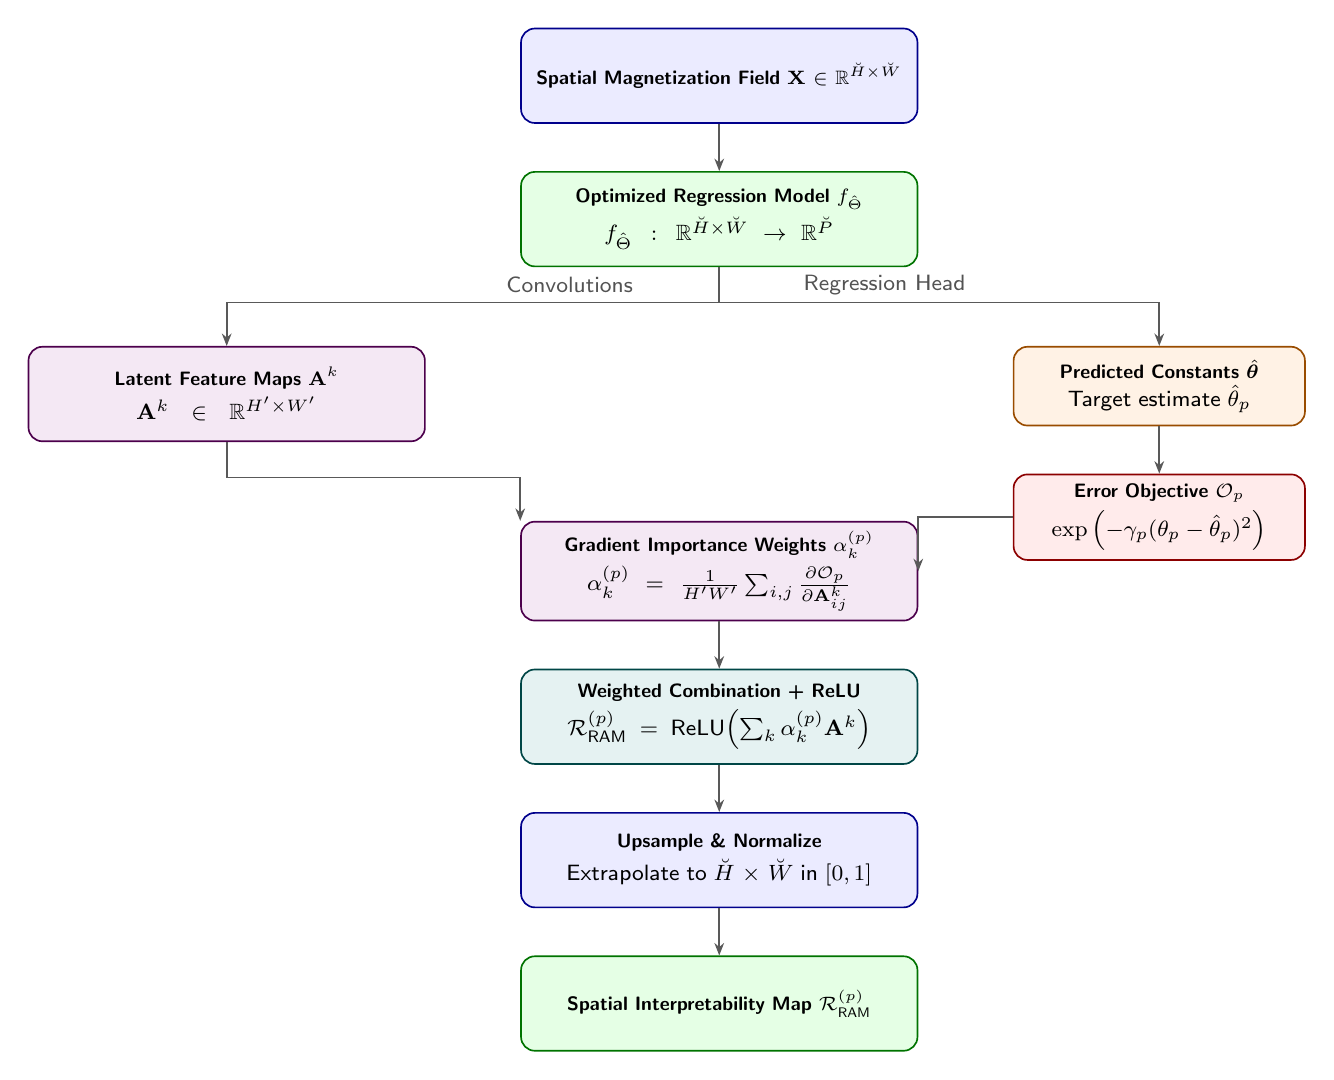
\begin{tikzpicture}[
      node distance = 0.6cm and 1.0cm,
      every node/.style = {font=\scriptsize\sffamily},
      blk/.style = {
        rectangle, rounded corners=5pt,
        minimum width=5.0cm, minimum height=1.2cm,
        text centered, text width=4.8cm,
        draw, line width=0.6pt
      },
      blkN/.style = {
        rectangle, rounded corners=5pt,
        minimum width=3.7cm, minimum height=1.0cm,
        text centered, text width=2.8cm,
        draw, line width=0.6pt
      },
      cinput/.style  = {blk,  fill=blue!8,    draw=blue!55!black},
      cmodel/.style  = {blk,  fill=green!10,  draw=green!45!black},
      cfeat/.style   = {blk,  fill=violet!9,  draw=violet!60!black},
      cpred/.style   = {blkN, fill=orange!10, draw=orange!60!black},
      cerror/.style  = {blkN, fill=red!8,     draw=red!55!black},
      cgrad/.style   = {blk,  fill=violet!9,  draw=violet!60!black},
      crelu/.style   = {blk,  fill=teal!10,   draw=teal!55!black},
      cnorm/.style   = {blk,  fill=blue!8,    draw=blue!55!black},
      cout/.style    = {blk,  fill=green!10,  draw=green!45!black},
      arr/.style = {-{Stealth[length=4.5pt, width=3.5pt]},
                    line width=0.6pt, gray!70!black},
    ]
    \node[cinput] (input)
      {\textbf{Spatial Magnetization Field} $\mathbf{X} \in \mathbb{R}^{\breve{H} \times \breve{W}}$};
    \node[cmodel, below=of input] (model)
      {\textbf{Optimized Regression Model} $f_{\hat{\Theta}}$\\[2pt]
       {\footnotesize $f_{\hat{\Theta}}:\mathbb{R}^{\breve{H} \times \breve{W}}\!\to\!\mathbb{R}^{\breve{P}}$}};
    \node[cfeat, below left=1.0cm and 1.2cm of model] (feat)
      {\textbf{Latent Feature Maps} $\mathbf{A}^{k}$\\[2pt]
       {\footnotesize $\mathbf{A}^{k}\in\mathbb{R}^{H' \times W'}$}};
    \node[cpred, below right=1.0cm and 1.2cm of model] (pred)
      {\textbf{Predicted Constants} $\hat{\boldsymbol{\theta}}$\\[2pt]
       {\footnotesize Target estimate $\hat{\theta}_{p}$}};
    \node[cerror, below=0.6cm of pred] (error)
      {\textbf{Error Objective} $\mathcal{O}_{p}$\\[2pt]
       {\footnotesize $\exp\left(-\gamma_p (\theta_p - \hat{\theta}_p)^2\right)$}};
    \node[cgrad, below right=1.0cm and 1.2cm of feat] (grad)
      {\textbf{Gradient Importance Weights} $\alpha_{k}^{(p)}$\\[2pt]
       {\footnotesize $\alpha_{k}^{(p)}=\frac{1}{H' W'}
         \sum_{i,j}\frac{\partial\mathcal{O}_{p}}
         {\partial \mathbf{A}^{k}_{ij}}$}};
    \node[crelu, below=0.6cm of grad] (relu)
      {\textbf{Weighted Combination + ReLU}\\[2pt]
       {\footnotesize $\mathcal{R}_{\text{RAM}}^{(p)}=
         \text{ReLU}\!\left(\sum_{k}
         \alpha_{k}^{(p)} \mathbf{A}^{k}\right)$}};
    \node[cnorm, below=0.6cm of relu] (norm)
      {\textbf{Upsample \& Normalize}\\[2pt]
       {\footnotesize Extrapolate to $\breve{H} \times \breve{W}$ in $[0,1]$}};
    \node[cout, below=0.6cm of norm] (out)
      {\textbf{Spatial Interpretability Map} $\mathcal{R}_{\text{RAM}}^{(p)}$};
    \draw[arr] (input) -- (model);
    \draw[arr] (model.south) -- ++(0,-0.45) -| (feat.north);
    \node[font=\footnotesize\sffamily, gray!65!black]
      at ($(model.south)+(-1.9,-0.22)$) {Convolutions};
    \draw[arr] (model.south) -- ++(0,-0.45) -| (pred.north);
    \node[font=\footnotesize\sffamily, gray!65!black]
      at ($(model.south)+(2.1,-0.22)$) {Regression Head};
    \draw[arr] (pred) -- (error);
    \draw[arr] (feat.south) -- ++(0,-0.45) -| (grad.north west);
    \draw[arr] (error.west) -- ++(0,0) -| (grad.east);
    \draw[arr] (grad) -- (relu);
    \draw[arr] (relu) -- (norm);
    \draw[arr] (norm) -- (out);
    \end{tikzpicture}
  }
  \caption{RAMs extraction pipeline. Latent feature maps and continuous predictions from the network backbone are explicitly coupled via an error-decay objective. Gradient-based importance weights combine these features to produce a normalized, physically traceable spatial saliency map for the target Hamiltonian parameter $\theta_{p}$.}
  \label{fig:rams_pipeline}
\end{figure*}


\subsubsection{RAMs for ViT-based Approaches}\label{sec:ViT_RAMs}
%ViT RAMs
While our standard RAMs formulation seamlessly integrates with CNNs by exploiting their innate spatial hierarchies, extending this interpretability metric to the Vision Transformers requires mapping sequence-based latent representations back to the two-dimensional physical domain. Unlike CNNs, which preserve spatial locality through sliding convolutional filters, the ViT processes the input spatial magnetization field $\mathbf{X}$ as a flattened sequence of $N_r$ non-overlapping patches, outputting a discrete sequence of latent embeddings. To evaluate ViT-based architectures within the exact same RAMs framework, we introduce a token-reshaping mechanism that bridges the one-dimensional transformer latent space with the two-dimensional topological geometry. Let the output of the terminal Transformer encoder block be denoted as $\mathbf{Z} \in \mathbb{R}^{(N_r + 1) \times D}$, where $D$ is the embedding dimension and the extra token corresponds to the global aggregation token (e.g., the \texttt{[CLS]} token) utilized by the regression head to predict the Hamiltonian parameters $\hat{\mathbf{y}}$. By isolating the $N_r$ spatial tokens, we obtain the localized sequence $\mathbf{Z}_s \in \mathbb{R}^{N_r \times D}$. Because each sequence token explicitly corresponds to a fixed physical patch of the original nanodot domain, $\mathbf{Z}_s$ can be folded back into a 2D spatial grid. Assuming square patches, the sequence is reshaped into a pseudo-feature map:

\begin{equation}\label{eq:ViT_Reshape}
\mathbf{A}_{\text{ViT}} = \text{Reshape}(\mathbf{Z}_s) \in \mathbb{R}^{\sqrt{N_r} \times \sqrt{N_r} \times D}.
\end{equation}

Once projected into this tensor format, $\mathbf{A}_{\text{ViT}}$ functions structurally identically to the terminal convolutional feature map $\mathbf{A}$ utilized in the CNN baseline. The $k$-th slice of the embedding dimension ($k \in \{1, \dots, D\}$) forms the latent spatial map $\mathbf{A}_{\text{ViT}}^k \in \mathbb{R}^{\sqrt{N_r} \times \sqrt{N_r}}$. We then apply the identical scale-invariant, error-based activation objective $\mathcal{O}_p$ defined in Equation~\ref{eq:RAM_Objective}. The spatial importance weights for the ViT embeddings are computed by globally averaging the gradients of this objective with respect to the reshaped spatial tokens:

\begin{equation}\label{eq:ViT_Weights}
\alpha_k^{(p)} = \frac{1}{N_r} \sum_{i=1}^{\sqrt{N_r}} \sum_{j=1}^{\sqrt{N_r}} \frac{\partial \mathcal{O}_p}{\partial (\mathbf{A}_{\text{ViT}})_{ij}^k}.
\end{equation}

RAMs for the ViT are constructed via the ReLU-activated linear combination of these reshaped embedding slices, precisely mirroring Equation~\ref{eq:RAM_Formulation}, before being upsampled to the original input resolution $\breve{H} \times \breve{W}$. This extension guarantees an architecture-agnostic evaluation of interpretability, ensuring that the isolated degenerate textures driving the model's predictions can be fairly compared across fundamentally disparate deep learning architectures.

\subsubsection{Normalized RAMs for Layer-Wise and Target-Specific Analysis}\label{sec:Nor_RAMs}

To rigorously compare the spatial activations across different Hamiltonian parameters and network depths, it is imperative to compute the RAMs utilizing strictly normalized predictions and targets. Let $\bar{\theta}_p \in [0,1]$ and $\hat{\bar{\theta}}_p \in [0,1]$ denote the Min-Max normalized ground truth and predicted values for the $p$-th physical parameter, respectively. By scaling the variables to a uniform interval, the layer-specific error objective is strictly bounded and evaluated as $\mathcal{O}_p = \exp(-\gamma_p (\bar{\theta}_p - \hat{\bar{\theta}}_p)^2)$. For a given convolutional or transformer layer $l \in \{1, \dots, L\}$, we extract the layer-specific unnormalized RAM, denoted as $\mathcal{R}_{\text{RAM}}^{(l,p)}$, following the gradient and activation protocols established in Equations~\ref{eq:RAM_Weights} and \ref{eq:RAM_Formulation}. To quantitatively evaluate and isolate the relative contribution of each distinct layer to the estimation of every physical constant, we introduce a global cross-layer and cross-parameter normalization scheme. The globally normalized activation map, $\tilde{\mathcal{R}}_{\text{RAM}}^{(l,p)}\in[0,1]$, is defined by scaling the layer-specific maps against the absolute maximum spatial activation observed across all $L$ layers and all $\breve{P}$ parameters:

\begin{equation}\label{eq:RAM_Global_Norm}
\tilde{\mathcal{R}}_{\text{RAM}}^{(l,p)} = \frac{\mathcal{R}_{\text{RAM}}^{(l,p)}}{\max\limits_{l' \in \{1,\dots,L\}, p' \in \{1,\dots,\breve{P}\}} \left( \max\limits_{i,j} \left[ \mathcal{R}_{\text{RAM}}^{(l',p')}\right]_{i,j} \right)}.
\end{equation}

This comprehensive normalization ensures that the gradient magnitudes are dimensionally consistent and comparable, preventing parameters with intrinsically higher variance or layers with larger gradient flows from disproportionately dominating the interpretability metrics. By tracking the evolution of $\tilde{\mathcal{R}}_{\text{RAM}}^{(l,p)}$ across the network depth, this formulation explicitly reveals how the deep learning architecture bypasses the intrinsically ill-conditioned nature of the inverse problem. In magnetic nanodots, severe structural ambiguity arises because disparate energetic combinations of the symmetric exchange ($\tilde{J}$), DMI ($\tilde{K}_{DM}$), magnetocrystalline anisotropy ($\tilde{K}$), and Zeeman field ($\tilde{H}_{ex}$) can yield highly degenerate states with nearly identical free energies. Then, the global normalization aim to code how the network dynamically resolves this degeneracy through a hierarchical physical decoupling. We establish that early network layers (lower $l$) exhibit high relative activations for parameters governing short-range spin interactions, capturing the localized chiral winding angles and domain wall boundaries dictated primarily by the delicate competition between $\tilde{J}$ and $\tilde{K}_{DM}$. Conversely, deeper layers (higher $l$) aggregate these localized topological textures to resolve macro-scale thermodynamic stability, with the terminal layers concentrating their activations on the globally-coupled parameters---most notably the annealing temperature $T^{(0)}$ and the exchange and field terms that govern the overall degree of order, phase transitions, and spatial alignment of emergent structures such as skyrmion cores and labyrinthine patterns. By correlating the intensity and spatial localization of $\tilde{\mathcal{R}}_{\text{RAM}}^{(l,p)}$ across the network hierarchy, our framework utilizes both localized boundary chirality and global domain spacing to disambiguate the underlying Hamiltonian parameters.

\subsubsection{Perturbation-Based Attribution Baselines}\label{sec:xai_baselines}

To rigorously assess the RAMs formulation, we benchmark it against three model-agnostic attribution methods adapted here to the continuous regression setting: the Local Interpretable Model-agnostic Explanations (LIME), the Shapley Additive Explanations (SHAP) in their kernel form over superpixels, and a spatial-frequency Shapley estimator (SF-SHAP) that evaluates exact Shapley values over a compact set of radial frequency bands. For a target parameter $p$, let $f_p : \mathbb{R}^{\breve{H} \times \breve{W}} \rightarrow \mathbb{R}$ denote the scalar map returning the $p$-th predicted parameter, $f_p(\mathbf{X}) = \hat{\theta}_p$. The input image is partitioned into $d$ disjoint interpretable regions (superpixels) $\{\mathcal{X}_1, \dots, \mathcal{X}_d\}$ obtained by spatial segmentation. A coalition vector $\mathbf{z} \in \{0,1\}^d$ encodes which regions are retained ($z_i = 1$) or masked to a reference baseline $b$ ($z_i = 0$), and the map $h_{\mathbf{X}}(\mathbf{z})$ reconstructs the corresponding perturbed image.

\emph{LIME.} This method fits a sparse linear surrogate $g(\mathbf{z}) = \phi_0 + \sum_{i=1}^{d} \phi_i z_i$ that locally approximates $f_p$ in the neighborhood of $\mathbf{X}$, by minimizing a proximity-weighted least-squares objective:

\begin{equation}\label{eq:lime}
\boldsymbol{\phi}^{\text{LIME}} = \arg\min_{g}\ \sum_{\mathbf{z}} \pi_{\mathbf{X}}(\mathbf{z})\,\big(f_p(h_{\mathbf{X}}(\mathbf{z})) - g(\mathbf{z})\big)^2 + \Omega(g),
\end{equation}
where $\pi_{\mathbf{X}}(\mathbf{z})$ is a proximity kernel that weights each perturbation by its similarity to the original image, and $\Omega(g)$ penalizes surrogate complexity to enforce sparsity. The coefficient $\phi_i$ is taken as the attribution of region $i$.

\emph{SHAP.} Grounded in cooperative game theory, the Shapley value attributes to each region $i$ the average marginal contribution it makes to the prediction across all possible coalitions:

\begin{equation}\label{eq:shap}
\phi_i = \sum_{\mathcal{S} \subseteq \mathcal{I} \setminus \{i\}} \frac{|\mathcal{S}|!\,(d - |\mathcal{S}| - 1)!}{d!} \Big( f_p\big(h_{\mathbf{X}}(\mathbf{z}_{\mathcal{S} \cup \{i\}})\big) - f_p\big(h_{\mathbf{X}}(\mathbf{z}_{\mathcal{S}})\big) \Big),
\end{equation}
where $\mathcal{I} = \{1, \dots, d\}$ and $\mathbf{z}_{\mathcal{S}}$ is the coalition activating only the regions in $\mathcal{S}$. This attribution is the unique one satisfying local accuracy, missingness, and consistency, but its exact evaluation requires $2^{d}$ model queries. Since $d$ equals the number of superpixels, exact enumeration is intractable, and SHAP therefore estimates the Shapley values through the kernel formulation---a weighted linear regression over sampled coalitions using the Shapley kernel

\begin{equation}\label{eq:kernelshap}
\pi_{\text{SHAP}}(\mathbf{z}) = \frac{d - 1}{\binom{d}{|\mathbf{z}|}\,|\mathbf{z}|\,(d - |\mathbf{z}|)},
\end{equation}
so that $\boldsymbol{\phi}^{\text{SHAP}} = \arg\min_{\boldsymbol{\phi}} \sum_{\mathbf{z}} \pi_{\text{SHAP}}(\mathbf{z}) \big( f_p(h_{\mathbf{X}}(\mathbf{z})) - \phi_0 - \sum_i \phi_i z_i \big)^2$; the resulting coefficients converge to the Shapley values of Equation~\ref{eq:shap} while sampling only a subset of coalitions.

\emph{SF-SHAP.} Rather than segmenting the image into superpixels, this variant partitions it into a small number $Q$ of concentric radial frequency bands, matched to the characteristic spatial scales of the magnetic texture. Because $Q$ is small ($Q=7$ here), the full coalition space of $2^{Q}=128$ subsets can be enumerated exactly, so SF-SHAP evaluates the Shapley values of Equation~\ref{eq:shap} without sampling approximation, at the cost of a coarser, frequency-resolved (rather than pixel-resolved) attribution.

Crucially, all three baselines are perturbation-based: each explanation demands hundreds to thousands of forward evaluations of $f_p$ to probe the coalition space, whereas a RAM is obtained from a single backward pass through the network.

To quantitatively and fairly compare the spatial faithfulness of every attribution method---RAMs and the perturbation baselines alike---we adopt a deletion protocol based on the \emph{Most Relevant First} (MoRF) criterion. Given the relevance map produced by a method $m$ for the parameter $p$, the $\breve{H}\breve{W}$ input locations are ranked in order of decreasing relevance, yielding the ordering $\pi_1^{(m)}, \pi_2^{(m)}, \dots, \pi_{\breve{H}\breve{W}}^{(m)}$. For a deletion fraction $\rho \in [0, \rho_{\max}]$, the $\lfloor \rho\,\breve{H}\breve{W} \rfloor$ most relevant locations are replaced by the reference baseline $b$, producing the perturbed image $\mathbf{X}^{(m)}(\rho)$, and the induced deviation of the prediction is measured as

\begin{equation}\label{eq:deletion_dev}
\Delta_p^{(m)}(\rho) = \big| f_p\big(\mathbf{X}^{(m)}(\rho)\big) - f_p(\mathbf{X}) \big|.
\end{equation}

A faithful attribution concentrates relevance on the locations that genuinely drive the prediction, so that removing them induces a large and rapid deviation. The overall faithfulness of method $m$ for parameter $p$ is therefore summarized by the area under the deletion curve,

\begin{equation}\label{eq:deletion_auc}
\text{AUC}_p^{(m)} = \int_0^{\rho_{\max}} \Delta_p^{(m)}(\rho)\, d\rho,
\end{equation}

where a larger $\text{AUC}_p^{(m)}$ indicates a more spatially localized and physically faithful explanation; a random-relevance map is included as a lower-bound control. This deletion score, together with the per-explanation computational cost, provides the quantitative basis for the interpretability comparison reported in Section~\ref{sec:results_dis}.


\section{Experimental Set-Up}\label{sec:experiments}

To evaluate the effectiveness of the proposed framework 
for Hamiltonian parameter estimation, we design a 
comprehensive experimental protocol that integrates 
physics-based simulations, data-driven modeling, and 
interpretability analysis. The objective of this setup 
is to systematically assess not only the predictive 
performance of the model, but also its ability to 
generalize across different physical regimes and provide 
meaningful spatial explanations through the proposed RAMs. 
The dataset utilized in this study consists entirely of 
simulated magnetic domain configurations generated through 
our atomistic Monte Carlo framework, as described in 
Section~\ref{sec:montecarlo_sim}. To accurately reflect 
the finite-size effects and surface boundaries inherent 
to experimental nanostructures, the magnetic nanodots 
were modeled on a three-dimensional discrete lattice. 
The cylindrical geometry was constrained by a radius of 
$R_d = 18.25$~[MUC] and a thickness of $\breve{L} = 5$~[MUC]. 
Within this confined grid, the spatial bounds were 
dictated by a strictly defined circular binary mask, 
yielding an active interacting volume of approximately 
5,200 localized spins per simulated dot.

For each unique combination of Hamiltonian parameters, 
the system was subjected to a rigorous simulated annealing 
protocol to isolate the thermodynamically relaxed state. 
To guarantee full ergodicity, the exchange-normalized 
initial temperature was established at an effective 
paramagnetic ceiling. The system was systematically 
cooled to a near-ground state of $T^{(f)} = 0.1$~K 
utilizing a linear decrement of $\Delta T = -0.1$~K. 
At each discrete temperature interval, the spin lattice 
underwent $10{,}000$ Monte Carlo Sweeps (MCS) exclusively
dedicated to thermalization, thereby overcoming metastable
localized energetic barriers. This thermalization phase
was subsequently followed by $2{,}000$ measurement MCS to
compute macroscopic thermodynamic averages (e.g., specific 
heat and magnetic susceptibility) and verify strict 
energetic convergence. To overcome the prohibitive 
computational bottleneck traditionally associated with 
sequential Monte Carlo methods, the atomistic simulation 
was rigorously optimized implemented in JAX as a fully vectorized, just-in-time-compiled routine distributed across multiple GPUs via single-program multiple-data (\texttt{pmap}) parallelism in single precision.

Upon converging to \ch{a low-energy thermodynamically stable state} at $0.1$~K, 
the final topological state was isolated. To mimic 
experimental 2D observation techniques, the spatial 
magnetization field was extracted exclusively from the 
central discrete layer of the nanodot 
($z = \lfloor \breve{L}/2 \rfloor$). The out-of-plane 
spin components ($s_z \in [-1, 1]$) were systematically 
normalized to the strict interval $[0, 1]$ and mapped 
onto a Cartesian pixel grid, finalizing the input images 
$\mathbf{X}$ corresponding to the specific physical 
targets $\boldsymbol{\theta}$. The extended Hamiltonian 
parameter vector $\boldsymbol{\theta} \in \mathbb{R}^8$ 
estimated in this study is defined as:
$\boldsymbol{\theta} = \bigl[T^{(0)},\, \tilde{J}_2,\, 
\tilde{J}_3,\, \tilde{J}_4,\, \tilde{K}_{an1},\, 
\tilde{K}_{anS},\, \tilde{H}_{ex},\, 
\tilde{K}_{DM}\bigr]$,
where the first-shell exchange constant $\tilde{J}_1 = 
1.0$~meV is fixed as the energy reference scale to 
break the scale symmetry of the inverse problem and 
ensure a well-posed regression target, as described 
in Section~\ref{sec:hamiltonian}. Each of the eight
free parameters was drawn with a quasi-random
(low-discrepancy) sampling scheme within the physically
motivated bounds summarized in
Table~\ref{tab:param_ranges}, ensuring a systematic and
homogeneous coverage of the admissible parameter region.

It is important to note that while all eight parameters
are simultaneously estimated by the regression models,
their effective identifiability from the $s_z$
projection varies substantially due to the physical
constraints of the observational modality. Six of the
eight parameters---the annealing temperature $T^{(0)}$,
the second-shell exchange $\tilde{J}_2$, the DMI strength
$\tilde{K}_{DM}$, the bulk and surface anisotropy
constants $\tilde{K}_{an1}$ and $\tilde{K}_{anS}$, and the
external field $\tilde{H}_{ex}$---are effectively
recovered from the two-dimensional projection. This is
made possible by the deliberate enrichment of the dataset:
applying the external field along the out-of-plane axis in
part of the simulations couples the Zeeman term directly
to the observable $s_z$ component, while the extended
anisotropy range produces sufficiently distinct domain-wall
morphologies for the anisotropy constants to leave a
measurable spatial signature. In contrast, the
higher-order exchange constants $\tilde{J}_3$ and
$\tilde{J}_4$ remain essentially unidentifiable: their
energetic contributions are strongly dominated by the
first- and second-shell interactions $\tilde{J}_1$ and
$\tilde{J}_2$, rendering their individual spatial
signatures indistinguishable in the magnetization texture.
These two constants are nevertheless retained in the
regression target $\boldsymbol{\theta}$ to provide a
complete and physically honest characterization of the
inverse problem, explicitly delineating its fundamental
identifiability limits rather than concealing them. Their
inclusion does not degrade the accuracy of the six
recoverable parameters, since the multi-output regression
head learns to allocate gradient capacity independently
to each output dimension. The resulting dataset is
publicly available and can be accessed through the
Kaggle repository%
\footnote{\url{https://www.kaggle.com/datasets/carloscanamejoy/dataset-spines-complete}}. 
It contains a total of $166{,}141$ samples, where 
each input is a grayscale magnetic domain image of 
size $39 \times 39 \times 1$ pixels, and each 
corresponding target is a vector of eight physical
parameters $\boldsymbol{\theta} \in \mathbb{R}^8$
as defined above.

To broaden the structural diversity of the dataset beyond a single field geometry, the external field orientation was varied within the dataset: in addition to the in-plane configuration, an out-of-plane field was employed to stabilize additional topologies such as isolated skyrmions, while the magnetocrystalline anisotropy range was deliberately extended toward high values to access an Ising-like regime characterized by sharper, more discrete domain walls. The dataset also spans two complementary mechanisms for stabilizing modulated, non-collinear textures: a chiral regime driven by the DMI $\tilde{K}_{DM}$ and an exchange-frustration regime driven by the second-shell exchange $\tilde{J}_2$. To isolate the contribution of each mechanism, these two interactions are activated in a mutually exclusive fashion across the sampled configurations. Consequently, in the pairwise correlation matrix of the eight parameters, $\tilde{J}_2$ and $\tilde{K}_{DM}$ are the only pair exhibiting an appreciable anti-correlation ($\rho \approx -0.53$)---a direct consequence of this deliberate design---while all remaining pairs are essentially uncorrelated ($|\rho| \lesssim 0.3$), confirming that the model cannot exploit spurious cross-parameter correlations to infer one parameter from another. This controlled heterogeneity enriches the space of magnetic phases that the regression models must disentangle and, together with the sampling bounds of Table~\ref{tab:param_ranges}, exposes the models to a wide range of competing energetic regimes within a single unified dataset.

The sampling bounds of Table~\ref{tab:param_ranges} are not intended to reproduce a single specific compound but to cover the region of Hamiltonian space where chiral and modulated magnetic textures exist. Since $\tilde{J}_1$ is fixed as the energy reference, the physically meaningful quantities are the dimensionless ratios $\tilde{J}_r/\tilde{J}_1$, $\tilde{K}_{DM}/\tilde{J}_1$, and $\tilde{K}/\tilde{J}_1$, and these ratios fall within the ranges reported by first-principles calculations and experiments for chiral magnets and ultrathin transition-metal films. The higher-order exchange constants ($|\tilde{J}_2|>|\tilde{J}_3|>|\tilde{J}_4|$, with $\tilde{J}_2/\tilde{J}_1$ up to $0.66$) reproduce the decaying, sign-alternating exchange obtained from density-functional calculations of ultrathin films such as Fe/Ir(111) and Pd/Fe/Ir(111)~\cite{heinze2011spontaneous, dupe2014tailoring}, and lie in the strong-frustration regime of the classical $\tilde{J}_1$--$\tilde{J}_2$ model. For the DMI, we sample $\tilde{K}_{DM}/\tilde{J}_1$ up to $\approx 1.2$; while interfacial materials typically exhibit $\tilde{K}_{DM}/\tilde{J}_1 \sim 0.3$--$0.7$~\cite{heinze2011spontaneous}, larger ratios are the standard choice in finite-lattice Monte Carlo studies so that the helical period ($\lambda \propto \tilde{J}_1/\tilde{K}_{DM}$) fits several times within the simulation cell~\cite{buhrandt2013skyrmion}. Because the physics is scale-invariant, a large ratio on a small lattice is equivalent to a small ratio in a large system, so this choice reflects standard finite-size rescaling rather than unphysical parameter values. The anisotropy range (up to $\tilde{K}_{an1}\approx 4.6$~meV/atom) spans from soft magnets to the strongly anisotropic interfacial regime, consistent with values reported for systems ranging from FePt to single Co adatoms on Pt(111)~\cite{gambardella2003giant, johnson1996magnetic}. Finally, the Zeeman range ($\tilde{H}_{ex}$ up to $1.2$~meV/atom) corresponds, through $E = g\mu_B B$ with $g\approx2$, to magnetic fields up to $\approx 10$~T---the upper range of standard laboratory magnets used to map skyrmion phase diagrams---and the temperature range ($T^{(0)}$ up to $20$~K, i.e., $k_B T/\tilde{J}_1$ up to $\approx1.7$) sweeps the system from the ordered ground state through the paramagnetic transition, consistent with ordering temperatures of chiral magnets with $\tilde{J}_1\sim1$~meV.

\begin{table}[h]
\centering
\caption{Sampling ranges for the eight free Hamiltonian 
parameters constituting the regression target 
$\boldsymbol{\theta}$. The first-shell exchange 
$\tilde{J}_1 = 1.0$~meV is fixed as the energy 
reference. Parameters are drawn with a quasi-random
(low-discrepancy) scheme within the specified bounds. Physical units:
temperature in Kelvin~[K], exchange and DMI constants 
in meV, anisotropy constants in meV/atom, external 
field in meV/atom.}
\label{tab:param_ranges}
\begin{tabular}{llcc}
\hline
\textbf{Parameter} & \textbf{Physical role} & 
\textbf{Min} & \textbf{Max} \\
\hline
$T^{(0)}$ [K]                & Annealing temperature  & $0.0$  & $20.0$ \\
$\tilde{J}_2$ [meV]          & 2nd-shell exchange     & $-0.33$ & $0.66$  \\
$\tilde{J}_3$ [meV]          & 3rd-shell exchange     & $-0.29$ & $0.29$  \\
$\tilde{J}_4$ [meV]          & 4th-shell exchange     & $-0.23$ & $0.24$  \\
$\tilde{K}_{an1}$ [meV/atom] & Bulk anisotropy        & $0.0$  & $4.57$  \\
$\tilde{K}_{anS}$ [meV/atom] & Surface anisotropy     & $0.0$  & $0.20$  \\
$\tilde{H}_{ex}$ [meV/atom]  & External Zeeman field  & $0.0$  & $1.20$  \\
$\tilde{K}_{DM}$ [meV]       & DMI strength           & $0.0$  & $1.20$  \\
\hline
\end{tabular}
\end{table}

\ch{It is important to note that the DMI strength $\tilde{K}_{DM}$ is sampled exclusively over non-negative values ($\tilde{K}_{DM} \in [0.0, 1.2]$~meV).  This restriction is a physically motivated convention arising from the symmetry properties of the antisymmetric exchange term in Equation~\ref{eq:Hamiltonian}. Under the transformation $\tilde{K}_{DM} \to -\tilde{K}_{DM}$, the equilibrium spin configuration undergoes a reversal of its in-plane chirality---the rotational sense of the chiral winding inverts---while the out-of-plane magnetization component $s_z$ at every lattice site remains strictly invariant. Since the regression models operate exclusively on the two-dimensional $s_z$ projection, configurations with $+\tilde{K}_{DM}$ and $-\tilde{K}_{DM}$ are exactly degenerate in the observation space, rendering the sign of the DMI fundamentally unidentifiable from $s_z$ images alone. Including both signs simultaneously would introduce a strict two-fold degeneracy in the input--output mapping, collapsing the model's predictions toward $\hat{\tilde{K}_{DM}} \approx 0$ and precluding meaningful regression. The chirality handedness is instead encoded through the fixed direction vector $\hat{\mathbf{d}}_{ij}$, consistent with standard conventions in atomistic modeling of interfacial DMI, where the sign of the antisymmetric exchange sets the preferred rotational sense of the chiral texture~\cite{fert2017magnetic, bogdanov1989thermodynamically, fillion2022gate}. Recovering the DMI sign would require access to chirality-sensitive observables, such as the full three-dimensional spin vector field or in-plane magnetization components, which constitutes a direction for future investigation (Section~\ref{sec:conclusions}).}

To ensure robust evaluation and prevent information 
leakage during the deep learning optimization phase, 
the generated dataset $\mathcal{D}$ is partitioned 
into training, validation, and testing subsets using 
a rigorous two-stage random split strategy. Initially, 
15\% of the total dataset is isolated as a hold-out 
test set to evaluate ultimate model generalization. 
Subsequently, the remaining 85\% is further divided, 
allocating exactly 15\% of the total initial data 
for validation. This procedure yields an effective 
split of 70\% for training, 15\% for validation, 
and 15\% for testing. All partitions are executed 
utilizing a fixed random seed to guarantee strict 
reproducibility across all experimental runs. This 
strategy ensures that topological samples remain 
strictly independent across subsets while perfectly 
preserving the underlying thermodynamic distributions 
of the dataset.

Prior to network ingestion, both the input spatial 
magnetization images and the target Hamiltonian 
variables are preprocessed to ensure numerical 
stability and efficient gradient convergence. The 
physical target variables are scaled using Min-Max 
normalization, mapping each continuous parameter to 
the strict interval $[0,1]$ based exclusively on the 
statistical distribution of the training set. This 
identical transformation is subsequently applied to 
the validation and test sets to maintain inferential 
consistency and directly support the bounded RAMs 
objective $\mathcal{O}_p \in (0,1]$. For the four deep backbone architectures, the single-channel $s_z$ 
matrices are spatially resized to $224 \times 224$ 
pixels and duplicated across three channels 
(grayscale-to-RGB conversion). This dimensional expansion matches the input dimensionality expected by the standard deep backbone architectures; the conventional CNN baseline instead operates directly on the native $39\times39\times1$ maps. No pretrained weights are used, and all architectures are trained entirely from scratch.

The configuration of the evaluated deep learning 
architectures (see Section~\ref{sec:Deep_Learning}) 
is summarized in Table~\ref{tab:model_config}. All five architectures share the same extended regression head designed 
to mitigate overfitting in the high-dimensional 
parameter space. Specifically, the global pooling 
output is passed through a Batch Normalization layer, 
followed by a Dropout layer with rate $p = 0.4$, a 
fully connected Dense layer of 256 units with ReLU 
activation and $\ell_2$ weight regularization 
($\lambda = 10^{-4}$), a second Batch Normalization 
layer, a second Dropout layer with rate $p = 0.3$, 
and a final linear Dense layer outputting the 
$\breve{P} = 8$ target parameters. For the convolutional architectures (the conventional CNN, ResNet50, DenseNet121, and Xception), the global aggregation is performed via 
Global Average Pooling over the spatial feature maps, 
whereas for the ViT-B/16 the token sequence output 
of the terminal encoder block is first collapsed via 
Global Average Pooling along the sequence dimension 
before entering the shared regularization head. This 
design choice reflects the distinct spatial inductive 
biases of convolutional and attention-based backbones 
while ensuring a strictly comparable regression 
capacity across all evaluated models.

\begin{table*}[!t]
\centering
\caption{Configuration of evaluated deep learning
architectures for inverse Hamiltonian parameter
estimation. All models share a standardized regularized
regression head mapped to the $\breve{P}=8$-dimensional
physical parameter space. BN: Batch Normalization;
Drop($p$): Dropout with rate $p$.}
\label{tab:model_config}
\resizebox{\textwidth}{!}{%
\begin{tabular}{lcccc}
\hline
\textbf{Model} & \textbf{Architecture Type} & 
\textbf{Pretraining} & \textbf{Global Aggregation} & 
\textbf{Output Head} \\
\hline
Conventional CNN & Custom CNN         & None (from scratch) &
  Global Avg.\ Pooling (spatial) &
  BN $\to$ Drop(0.4) $\to$ Dense(256, ReLU, $\ell_2$) $\to$ BN $\to$ Drop(0.3) $\to$ Dense(8) \\
ResNet50    & Residual CNN            & None (from scratch) &
  Global Avg.\ Pooling (spatial) &
  BN $\to$ Drop(0.4) $\to$ Dense(256, ReLU, $\ell_2$) $\to$ BN $\to$ Drop(0.3) $\to$ Dense(8) \\
DenseNet121 & Densely Connected CNN   & None (from scratch) & 
  Global Avg.\ Pooling (spatial) & 
  BN $\to$ Drop(0.4) $\to$ Dense(256, ReLU, $\ell_2$) $\to$ BN $\to$ Drop(0.3) $\to$ Dense(8) \\
Xception    & Depthwise Separable CNN & None (from scratch) & 
  Global Avg.\ Pooling (spatial) & 
  BN $\to$ Drop(0.4) $\to$ Dense(256, ReLU, $\ell_2$) $\to$ BN $\to$ Drop(0.3) $\to$ Dense(8) \\
ViT-B/16    & Patch-based Transformer & None (from scratch) &
  Global Avg.\ Pooling (tokens)  &
  BN $\to$ Drop(0.4) $\to$ Dense(256, ReLU, $\ell_2$) $\to$ BN $\to$ Drop(0.3) $\to$ Dense(8) \\
\hline
\end{tabular}}
\end{table*}

The optimization of the parameter set $\hat{\Theta}$ 
was executed utilizing the Adam optimizer with a 
unified initial learning rate of $\eta = 10^{-4}$ 
for all architectures, including the ViT-B/16, 
chosen for stable convergence when training all architectures from scratch. All models were trained 
to minimize the MSE loss function, while the MAE 
was actively monitored as a secondary diagnostic. 
Training was conducted using a highly parallelized 
batch size of $256$ samples over a maximum of 
100 epochs. To actively prevent overfitting and 
manage the learning dynamics within the highly 
degenerate optimization landscape, two primary 
callbacks were implemented: a dynamic learning 
rate scheduler (\texttt{ReduceLROnPlateau}) that 
reduced the learning rate by a factor of 0.3 if 
the validation loss stagnated for 5 consecutive epochs, and an \texttt{EarlyStopping} protocol 
that halted training and restored the best network 
weights if no validation improvement was observed 
after 12 consecutive epochs.

The predictive performance on the unseen test set 
was quantitatively assessed using two complementary 
regression metrics. The coefficient of determination 
($R^2$) quantifies the proportion of variance in 
each physical parameter successfully captured by 
the network:
%
\begin{equation}\label{eq:R2}
R^2 = 1 - \frac{\sum_{n=1}^{N_{\text{test}}} 
\left(\theta_{n,p} - \hat{\theta}_{n,p}\right)^2}
{\sum_{n=1}^{N_{\text{test}}} 
\left(\theta_{n,p} - \bar{\theta}_p\right)^2},
\end{equation}
%
where $\bar{\theta}_p$ is the mean of the observed 
ground truth target. Note that $R^2$ is statistically 
undefined when the target variable exhibits near-zero 
variance within a given evaluation subset; in these 
cases the metric is reported as N/A. The Mean Absolute 
Error (MAE) evaluates the absolute magnitude of the 
prediction error in the normalized feature space 
$[0,1]$, providing a direct and interpretable measure 
of per-parameter accuracy:
%
\begin{equation}\label{eq:MAE}
\text{MAE} = \frac{1}{N_{\text{test}}} 
\sum_{n=1}^{N_{\text{test}}} 
\left|\theta_{n,p} - \hat{\theta}_{n,p}\right|.
\end{equation}
%
Since all target variables are Min-Max normalized 
to $[0,1]$ prior to training, the MAE is inherently 
dimensionless and directly comparable across all 
eight Hamiltonian parameters, irrespective of their 
original physical units or numerical ranges.

The RAMs were computed on the held-out test set 
using the formulations introduced in 
Section~\ref{sec:RAMs}. For the Xception 
backbone, RAMs were extracted from eight layers 
selected to systematically cover the three 
functional stages of the architecture: two 
entry-flow layers capturing low-level spatial 
features at high resolution --- 
\texttt{block1\_conv2} ($112\times112$) and 
\texttt{block3\_sepconv2} ($56\times56$) ---; 
one transitional layer at 
\texttt{block4\_sepconv2} ($28\times28$); five 
middle-flow layers operating at the bottleneck 
resolution of $14\times14$ --- 
\texttt{block6\_sepconv2}, 
\texttt{block8\_sepconv2}, 
\texttt{block10\_sepconv2}, and 
\texttt{block12\_sepconv2} ---; and one 
exit-flow layer, \texttt{block13\_sepconv2} 
($14\times14$), immediately preceding the 
global pooling operation. This stratified 
selection was motivated by the physical 
hypothesis that early layers encode 
fine-grained domain periodicity and local 
spin-winding patterns at the scale of 
individual domain walls, while middle-flow 
layers progressively aggregate these local 
features into intermediate topological 
representations, and exit-flow layers encode 
high-level semantic information about the 
global magnetic phase. By distributing the 
selected layers across all three functional 
stages, the analysis directly tests whether 
the hierarchical decoupling predicted by the 
normalized RAM formulation of 
Equation~\ref{eq:RAM_Global_Norm} is 
empirically realized in the Xception backbone 
for Hamiltonian parameter estimation. For the 
ViT, a single attribution map per parameter 
was derived from the spatial token embeddings 
at the output of the terminal encoder block, 
reshaped into $\mathbf{A}_{\text{ViT}} \in 
\mathbb{R}^{14\times14\times768}$ following 
Equation~\ref{eq:ViT_Reshape}. Since 
\texttt{keras\_hub.ViTBackbone} does not expose 
internal token tensors as differentiable nodes 
within \texttt{tf.GradientTape}, the token 
sequence $\mathbf{Z}_s \in 
\mathbb{R}^{196\times768}$ was first extracted 
via a standard forward pass and then 
re-instantiated as a \texttt{tf.Variable} to 
enable gradient computation. The 
\texttt{[CLS]} token was treated as a fixed 
constant and the reconstructed sequence was 
passed through the \texttt{GlobalAveragePooling1D} 
and \texttt{Dense} regression head to compute 
$\mathcal{O}_p$ and its gradients with respect 
to $\mathbf{Z}_s$, following 
Equation~\ref{eq:ViT_Weights}.

The precision factor was fixed to 
$\gamma_p = 10$ uniformly for all 
$p \in \{1,\dots,8\}$. Given that all target 
variables are Min-Max normalized to $[0,1]$, 
this value ensures a smooth and well-conditioned 
gradient signal across the full prediction error 
range: $\mathcal{O}_p \geq e^{-10} \approx 
4.5\times10^{-5}$ at maximum error and 
$\mathcal{O}_p = 1$ at perfect prediction. 
Lower values of $\gamma_p$ would yield spatially 
diffuse attributions insensitive to prediction 
quality, while higher values would cause gradient 
saturation for the less identifiable parameters 
where errors are systematically larger. The 
chosen value maintains sensitivity across all 
eight parameters, from the most identifiable 
($T^{(0)}$, $\tilde{J}_2$, and $\tilde{K}_{DM}$) 
to the physically degenerate ones 
($\tilde{K}_{an1}$, $\tilde{K}_{anS}$, 
$\tilde{H}_{ex}$).

To confine activations to the physical extent 
of the nanodot, a circular binary mask 
$\mathcal{M}\in\{0,1\}^{224\times224}$ --- 
defined as a disk of radius $r = 0.94\times112$ 
pixels centered at the image center --- was 
applied to each RAM before normalization, 
setting all activations outside the disk to 
zero. A concentration score $\xi\in[0,1]$, 
measuring the fraction of total activation 
energy within the disk, was used to select 
the most physically representative sample per 
magnetic phase: among the ten test images 
closest to the UMAP centroid of each phase 
cluster, the sample maximizing $\bar{\xi}$ 
averaged over all parameters and layers was 
chosen as the phase representative 
$\mathbf{X}_n^*$.

All experiments were conducted in a cloud environment on RunPod. The computational 
setup was equipped with an NVIDIA H200 GPU. The training 
pipeline was implemented in Python using TensorFlow, 
leveraging GPU acceleration for efficient model training and inference. The atomistic state simulations were executed separately on the multi-GPU JAX configuration described in Section~\ref{sec:montecarlo_sim}. The complete source code 
is publicly available at 
\url{https://github.com/deathperminut/PaperInverseProblemEstimation}, 
organized into three modules: 
\texttt{/simulation} containing the atomistic 
Monte Carlo Hamiltonian simulation scripts 
implemented in JAX with multi-GPU (\texttt{pmap}) parallelization; \texttt{/regression} containing 
the training, validation, and evaluation pipelines
for all five deep learning architectures; and
\texttt{/rams} containing the Regression Activation 
Maps computation and visualization code for both 
the Xception CNN and the Vision Transformer.



\section{Results and Discussion}\label{sec:results_dis}

\subsection{Thermodynamic Simulation of Magnetic Topologies}
\label{sec:image_results}

%dataset statistics
We present the main results of the proposed atomistic Hamiltonian simulation framework (see Section~\ref{sec:materials}). The simulated dataset spans the eight-dimensional parameter space $\boldsymbol{\theta}$ over the bounds summarized in Table~\ref{tab:param_ranges}, sampled with deliberately heterogeneous densities: the higher-order exchange constants $\tilde{J}_2$, $\tilde{J}_3$, and $\tilde{J}_4$ concentrate near zero, whereas the DMI strength $\tilde{K}_{DM}$ is broadly populated across its full $[0, 1.2]$~meV range, and the bulk anisotropy $\tilde{K}_{an1}$ and external field $\tilde{H}_{ex}$ exhibit heavy tails toward high values that deliberately incorporate high-anisotropy, Ising-like regimes and out-of-plane field configurations. These bounded ranges and sampling heterogeneities explicitly govern the topological diversity of the generated magnetic phase space and, in turn, the learning dynamics, optimization stability, and predictive limits of the downstream deep regression frameworks when navigating the challenging regimes of the extended Heisenberg Hamiltonian.

%convergence monte carlo example
To further validate the physical consistency of the generated dataset and provide an intuitive understanding of the underlying spin dynamics, Figure~\ref{fig:convergence} illustrates the thermodynamic evolution of a representative magnetic nanodot during the Metropolis--Hastings Monte Carlo annealing process. This simulation is conducted under the fixed parameter configuration $\tilde{J}_1 = 1.0$~meV, $\tilde{J}_2 = \tilde{J}_3 = \tilde{J}_4 = 0.0$~meV, $\tilde{K}_{an1} = 0.10$~meV/atom, $\tilde{K}_{anS} = 0.00$~meV/atom, $\tilde{H}_{ex} = 0.00$~meV/atom, and $\tilde{K}_{DM} = 1.00$~meV, which constitutes a representative point within the full eight-dimensional parameter space $\boldsymbol{\theta}$ defined in Table~\ref{tab:param_ranges}. The vanishing values of the higher-order exchange constants ($\tilde{J}_2$, $\tilde{J}_3$, $\tilde{J}_4$), surface anisotropy ($\tilde{K}_{anS}$), and external field ($\tilde{H}_{ex}$) isolate the dominant energetic competition between the first-shell symmetric exchange $\tilde{J}_1$ and the DMI $\tilde{K}_{DM}$, making this configuration particularly illustrative of the chiral ordering mechanism. The main panel tracks the total Hamiltonian energy $\mathcal{H}$ [meV] as a function of the exchange-normalized annealing temperature $T^{(0)}$ [K], while each inset displays the corresponding two-dimensional out-of-plane magnetization field $s_z$ of the central layer at that specific thermal state. At elevated temperatures ($T^{(0)} \gtrsim 15$~K), the spin configurations exhibit a fully disordered, paramagnetic character, manifesting as spatially uncorrelated fluctuations of $s_z$ with no preferred orientation. As the system is progressively cooled through the intermediate regime ($5~\text{K} \lesssim T^{(0)} \lesssim 15$~K), short-range correlated domains begin to nucleate, reflecting the growing dominance of the symmetric exchange interaction $\tilde{J}_1$ over thermal fluctuations. In this regime, the competition between $\tilde{J}_1$ and the $\tilde{K}_{DM}$ progressively induced non-collinear and chiral spin winding, visible as the emergence of alternating red-blue stripe-like patterns. Upon convergence to the near-ground state at $T^{(0)} = 0.1$~K, the system stabilizes into a well-defined labyrinthine domain configuration, characteristic of the helical phase governed by a strong DMI relative to the exchange energy. The monotonic decrease $\mathcal{H}$ throughout the annealing trajectory confirms the thermodynamic relaxation of the system toward \ch{a low-energy stable configuration}, validating the physical correctness of the Monte Carlo pipeline and the quality of the generated dataset as input for the deep learning regression framework.

%Monte carlo convergence
\begin{figure*}[!t]
    \centering
    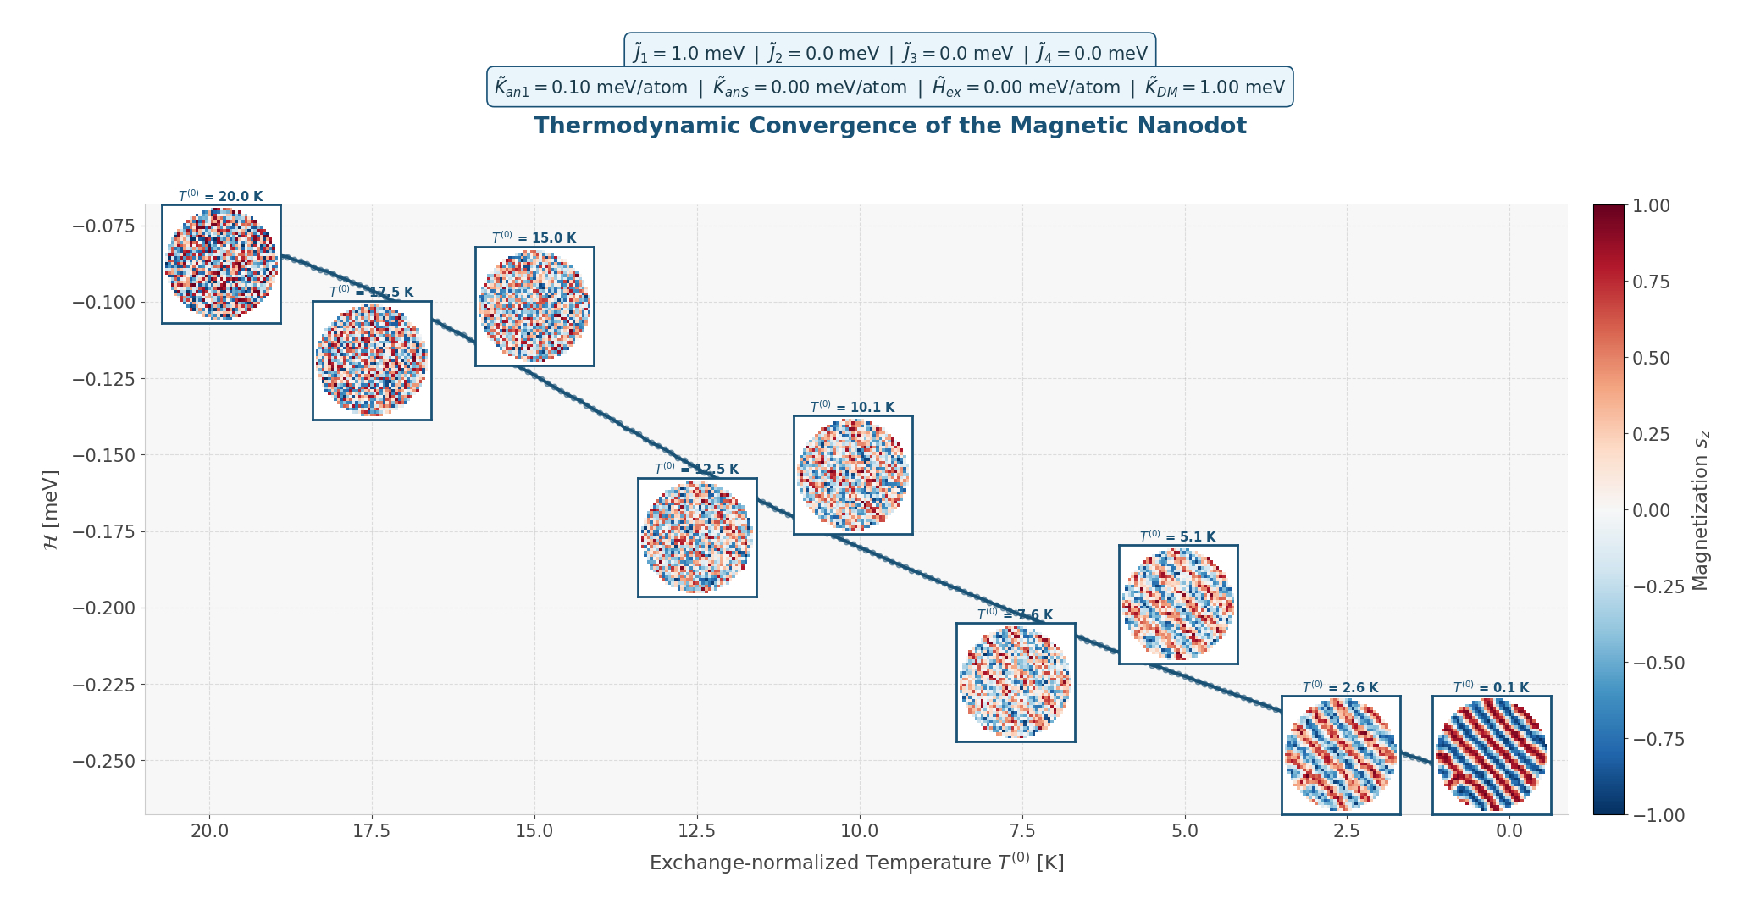
\includegraphics[width=\linewidth, trim=0 0 0 82bp, clip]{convergence}
    \caption{Thermodynamic convergence of a representative nanodot during simulated annealing. The main panel shows the total Hamiltonian energy $\mathcal{H}$ [meV] versus the annealing temperature $T^{(0)}$ [K]; each inset shows the $s_z$ field of the central layer at that state, tracing the transition from a disordered paramagnetic phase at high $T^{(0)}$ to a relaxed labyrinthine configuration at $T^{(0)} = 0.1$~K.}
    \label{fig:convergence}
\end{figure*}

To fully characterize the structural diversity generated by the Monte Carlo annealing protocol across the entire dataset, Figure~\ref{fig:phase_diagrams} presents two-dimensional phase diagrams of the magnetization image as a function of key Hamiltonian parameter pairs: $T^{(0)}$ versus $\tilde{J}_2$ and $T^{(0)}$ versus $\tilde{K}_{DM}$. These diagrams illustrate the macroscopic topological transitions driven by the underlying atomistic energetic competition. In the low-temperature regime, the system stabilizes into well-defined ordered textures whose morphology is dictated by the parameters: increasing $\tilde{K}_{DM}$ drives the sequence from nearly uniform ferromagnetic states, through chiral stripe and labyrinthine domains, to isolated skyrmionic textures, while the sign of $\tilde{J}_2$ separates ferromagnetic from antiferromagnetically modulated exchange ordering. Crucially, these ordered configurations remain visually distinguishable across the parameter space, which is precisely what allows the majority of the Hamiltonian parameters to be recovered by the inverse models. The principal source of ill-conditioning is instead thermal in origin: as the annealing temperature approaches the effective Curie point $T_C$, thermal fluctuations progressively overwhelm the magnetic interactions, and the system passes through transient, partially ordered states before collapsing into a paramagnetic, spatially uncorrelated texture that carries little discriminative information about the generating parameters. This temperature-driven loss of structure---together with the weakly discriminative transient regimes, rather than any intrinsic parameter degeneracy---constitutes the dominant challenge the dataset poses to the inverse estimation, consistent with the noisy, ill-conditioned regimes highlighted in the abstract. By comprehensively sampling this phase space, including these transient and high-temperature regimes, the thermodynamic simulation establishes a rich yet rigorously challenging foundation for the subsequent inverse deep learning parameter estimation.


\begin{figure*}[!t]
    \centering
    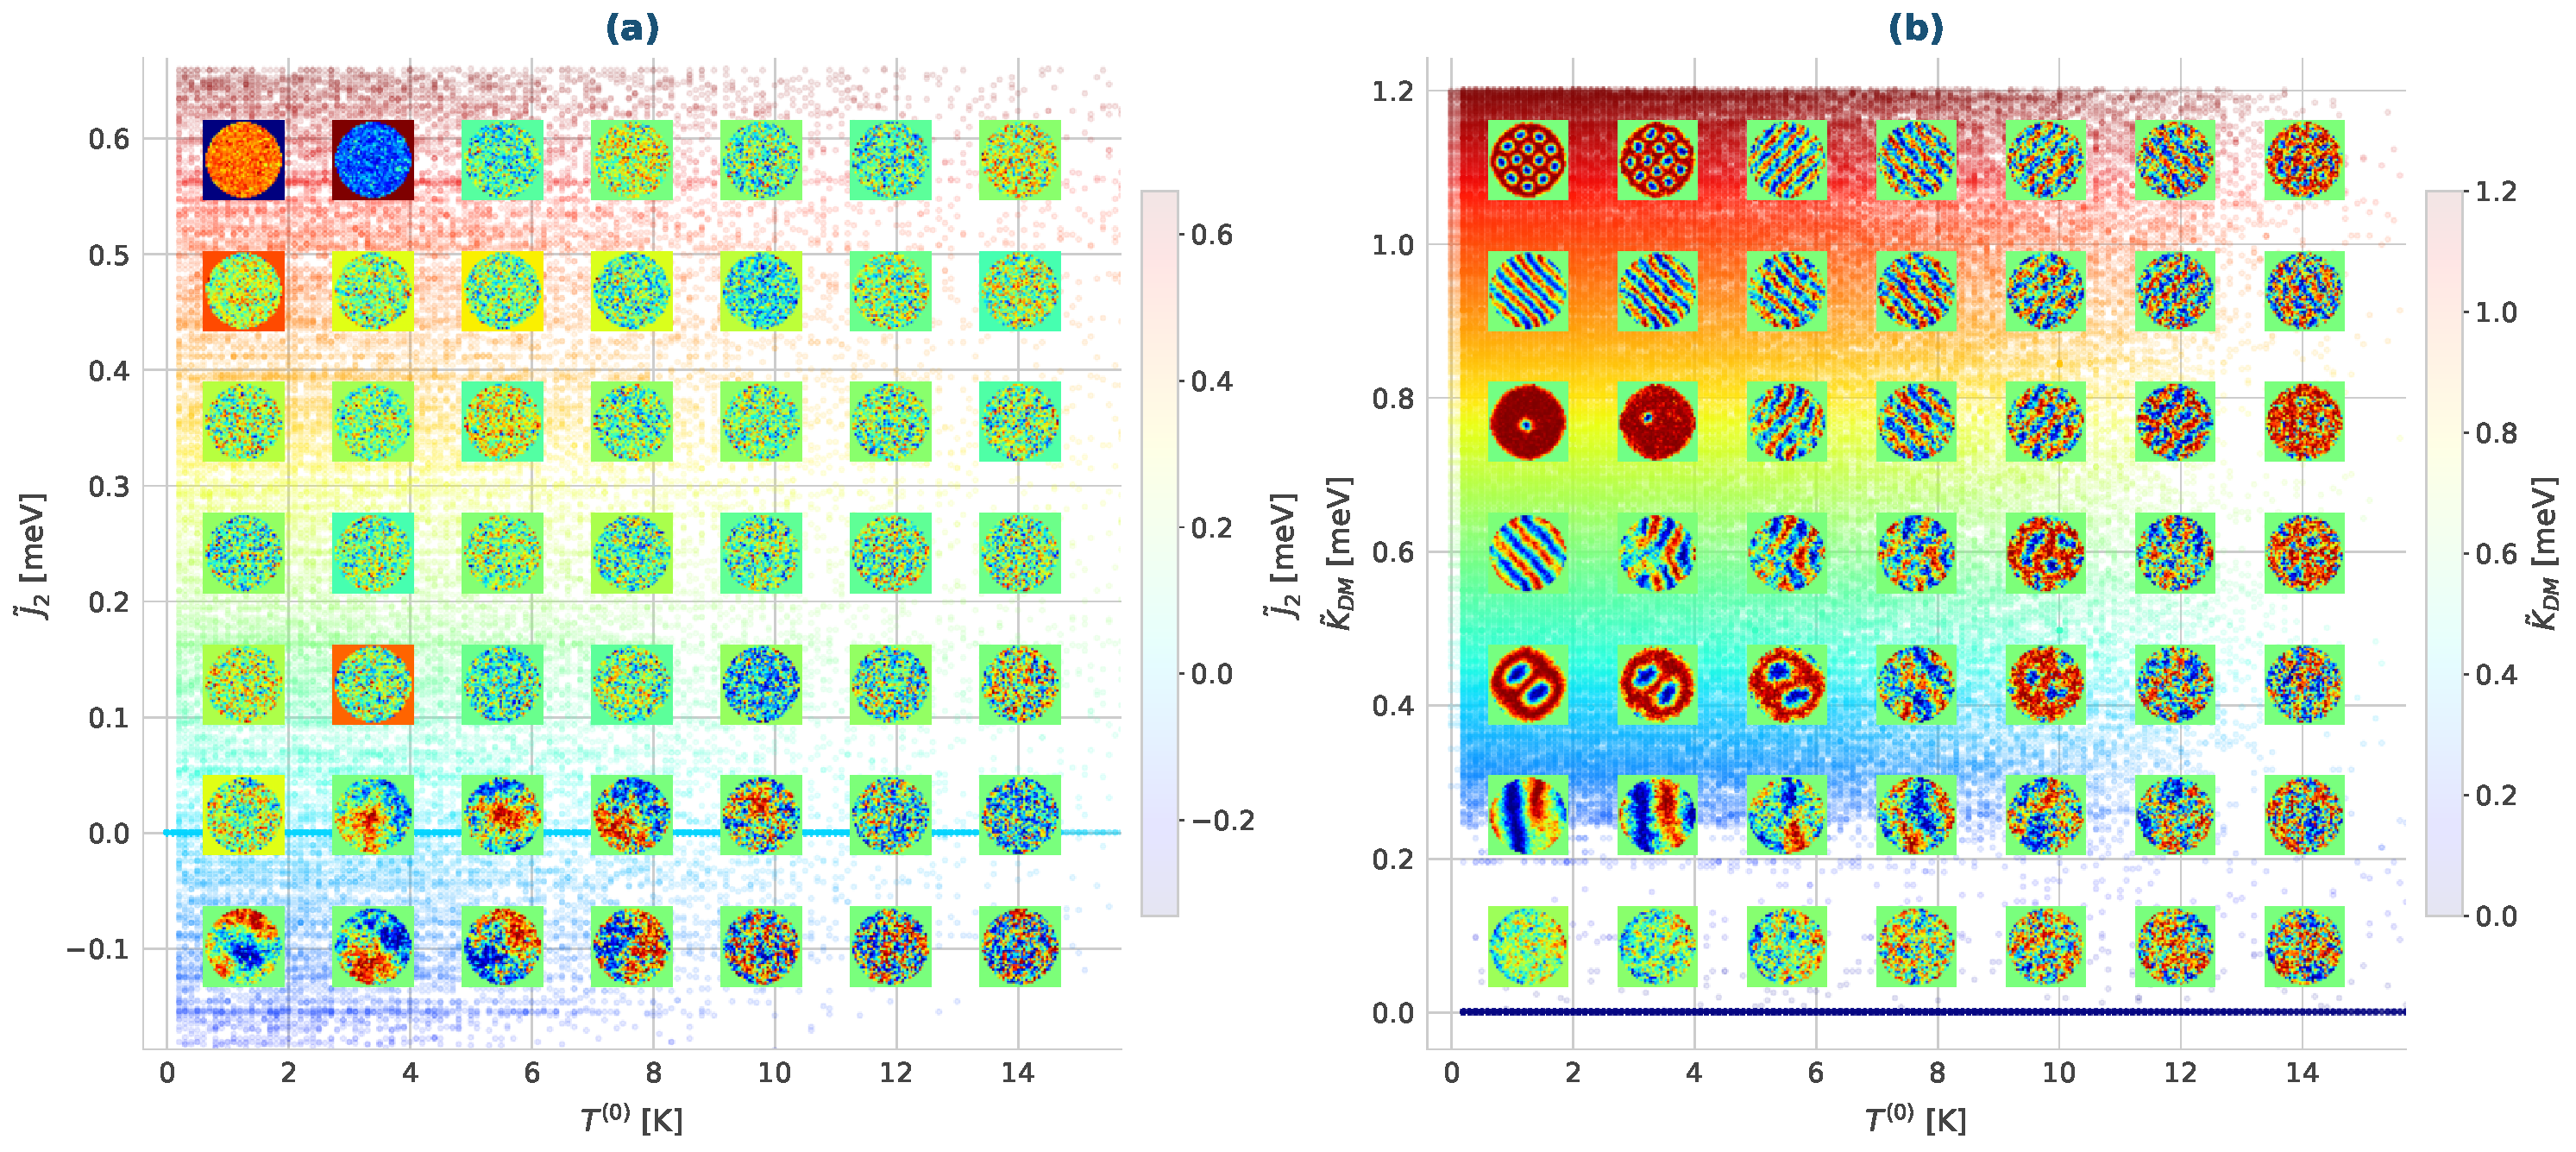
\includegraphics[width=\linewidth]{phase_diagrams}
    \caption{Two-dimensional phase diagrams of the magnetization
    texture $\mathbf{X}_n$ over parameter pairs:
    \textbf{(a)}~$T^{(0)}$ vs $\tilde{J}_2$ and
    \textbf{(b)}~$T^{(0)}$ vs $\tilde{K}_{DM}$. Each cell shows an
    enlarged representative image on a coarse sampling grid; the
    background color encodes the vertical-axis parameter.}
    \label{fig:phase_diagrams}
\end{figure*}


\subsection{Deep Learning Regression Results}\label{sec:dl_results}

The predictive performance of the five evaluated architectures (the
conventional CNN baseline, DenseNet, ResNet, Xception, and ViT) was
assessed on the held-out test set comprising 15\% of the total dataset.
Each model was tasked with simultaneously inferring the complete
extended parameter vector $\boldsymbol{\theta}$ directly from the
two-dimensional out-of-plane magnetization image $\mathbf{X}_n$,
without any auxiliary physical information. As shown in
Figures~\ref{fig:r2_metrics} and~\ref{fig:mae_metrics}, all five
architectures perform competitively, with the differences on the
identifiable parameters typically confined to a few percent of $R^2$.
Among them, Xception emerges as the strongest overall model: it attains
the highest $R^2$ for six of the eight parameters --- including the
most identifiable ones, $T^{(0)}$, $\tilde{J}_2$, $\tilde{K}_{an1}$,
and $\tilde{K}_{DM}$ --- while the ViT marginally leads on the external
field $\tilde{H}_{ex}$ and the conventional CNN baseline on the surface
anisotropy $\tilde{K}_{anS}$. The same ranking is largely mirrored in
the MAE panels, where Xception yields the lowest absolute error for the
physically dominant parameters $T^{(0)}$, $\tilde{K}_{an1}$, and
$\tilde{K}_{DM}$. A particularly informative observation is that the
conventional CNN baseline --- trained from scratch and devoid of
pretraining or specialized inductive biases --- matches, and for some
parameters even exceeds, the deeper backbones. This confirms that
neither transfer learning from natural images nor the sophisticated
residual, dense, depthwise, or attention mechanisms provide a decisive
advantage for this task; the estimation accuracy is instead governed by
the physical information that the $s_z$ projection makes available.
Physically, Xception's slight edge stems from its depthwise separable
convolution mechanism, which efficiently decouples the extraction of
spatial spin-texture frequencies from the cross-channel correlations
required to map those features onto the Hamiltonian parameter space,
yielding the most accurate point predictions for the dominantly
identifiable parameters. The ViT, in turn, remains competitive by
processing $\mathbf{X}_n$ as a sequence of non-overlapping spatial
patches and computing multi-head self-attention across all patch pairs,
explicitly capturing the long-range correlations---such as the global
chirality imposed by $\tilde{K}_{DM}$ and the large-scale ordering
driven by $\tilde{J}_1$---that are inaccessible to purely local
convolutional receptive fields.

This near-equivalence across architectures raises the question of
whether model capacity limits the estimation at all.
Figure~\ref{fig:accuracy_vs_size} plots the mean $R^2$ over the
identifiable parameters against the number of trainable weights of each
architecture, spanning nearly two orders of magnitude in model
size---from the compact conventional CNN ($\sim\!1$~M parameters) to the
ViT ($\sim\!86$~M parameters). The resulting trend is essentially flat:
the conventional CNN already attains a mean $R^2$ close to that of the
largest models, and increasing the parameter count by two orders of
magnitude yields only a marginal improvement, with Xception offering the
best accuracy--size trade-off. This saturation demonstrates that
predictive accuracy is not bottlenecked by model capacity but by the
physical information accessible in the $s_z$ projection: once an
architecture is expressive enough to read the relevant spatial features,
additional parameters and more elaborate inductive biases provide
diminishing returns, confirming that the recovery of the identifiable
parameters is a robust, architecture-independent property of the data.

\begin{figure}[htbp]
    \centering
    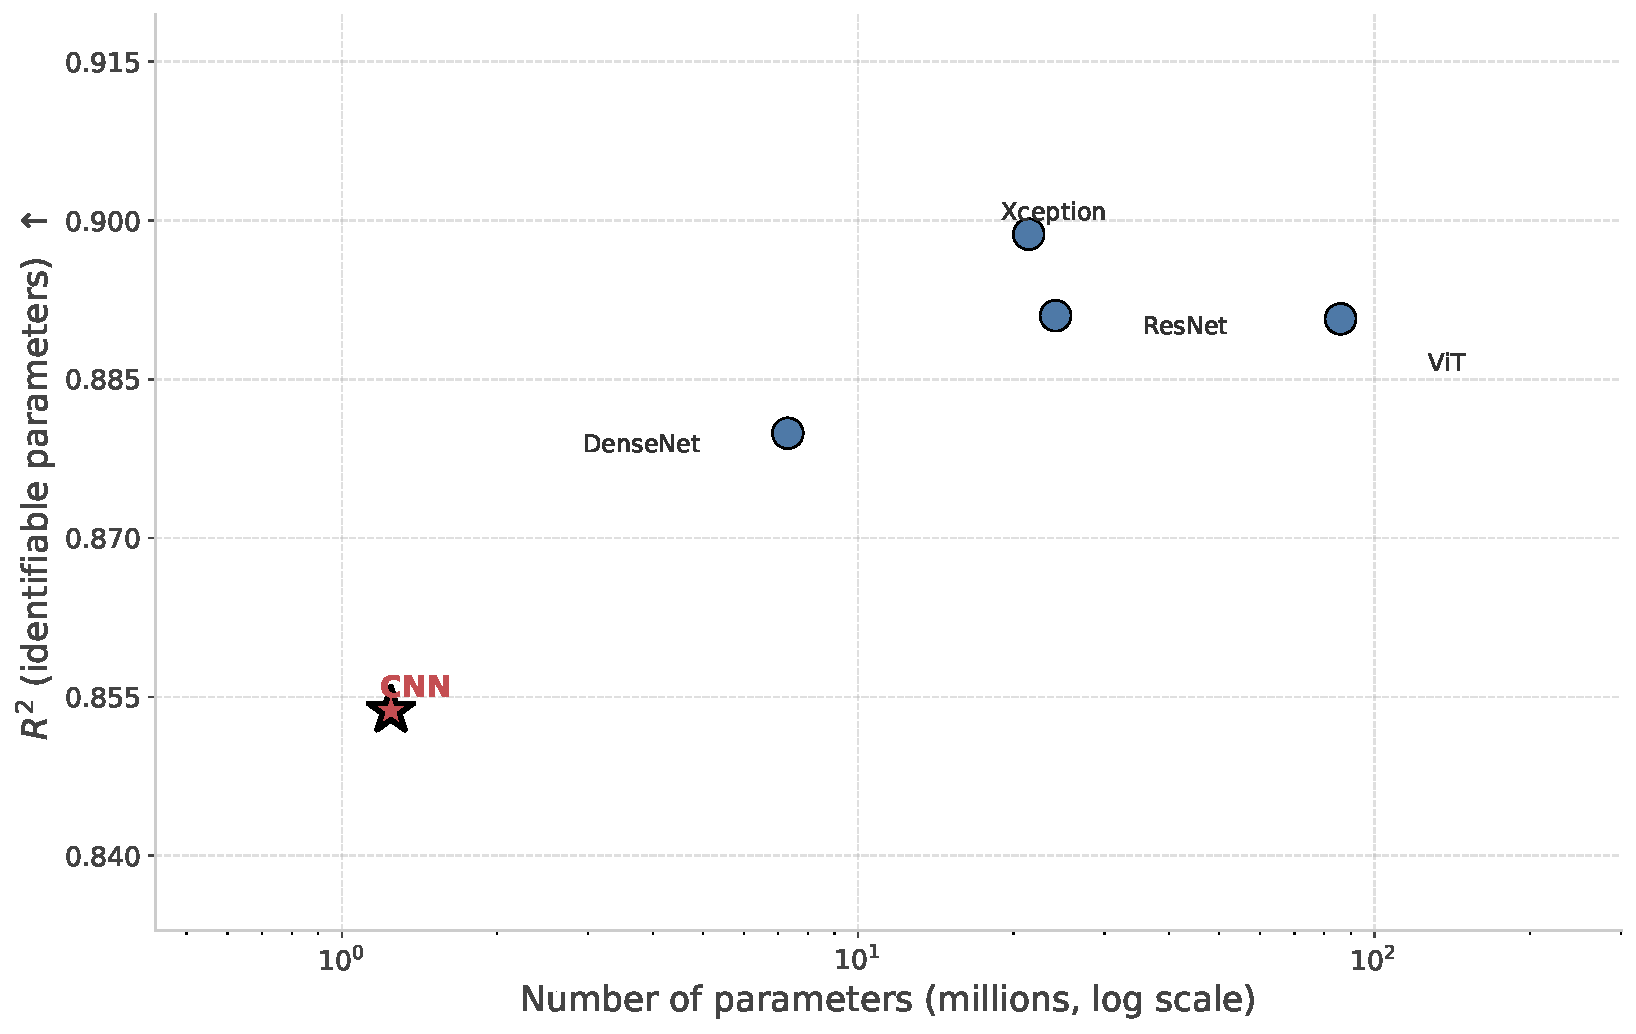
\includegraphics[width=\linewidth]{accuracy_vs_size-2}
    \caption{Mean $R^2$ over the identifiable Hamiltonian parameters
    versus the number of trainable weights (log scale) for the five
    architectures. The nearly flat trend---the compact CNN already
    matching models two orders of magnitude larger---indicates that
    accuracy is limited by the physical information in the $s_z$
    projection, not by model capacity.}
    \label{fig:accuracy_vs_size}
\end{figure}

Figures~\ref{fig:r2_metrics} and~\ref{fig:mae_metrics} reveal a
pronounced and physically interpretable heterogeneity in predictive
accuracy across the parameter space. The initial annealing temperature
$T^{(0)}$, the second-shell exchange $\tilde{J}_2$, the DMI strength
$\tilde{K}_{DM}$, the bulk anisotropy $\tilde{K}_{an1}$, and the
external field $\tilde{H}_{ex}$ consistently yield high $R^2$
scores across all architectures, reflecting the robust and spatially
distinctive topological imprints they leave on the observable
magnetization texture: $T^{(0)}$ governs the global degree of spin
order, $\tilde{J}_2$ controls the second-neighbor exchange pathway
that modulates the domain-scale collinearity, and $\tilde{K}_{DM}$
directly dictates the characteristic wavelength and chirality of the
domain patterns. However, a seemingly contradictory observation
emerges when examining the MAE panels in Figure~\ref{fig:mae_metrics}:
despite their high $R^2$ scores, $T^{(0)}$, $\tilde{J}_2$, and
$\tilde{K}_{DM}$ also exhibit comparatively larger absolute errors in
their respective physical units --- reaching up to approximately
$0.49\,\mathrm{K}$ for $T^{(0)}$, $0.021\,\mathrm{meV}$ for
$\tilde{J}_2$, and $0.037\,\mathrm{meV}$ for $\tilde{K}_{DM}$ in the
worst-performing architecture. This apparent inconsistency is not a
failure of the models but rather a direct consequence of the
thermodynamic landscape of the dataset. As illustrated in the phase
diagrams of Figure~\ref{fig:phase_diagrams}, the parameter space
contains extensive high-temperature regions where thermal
fluctuations above the effective Curie temperature $T_C$ collapse the
magnetization texture into an indistinguishable paramagnetic noise
regime, regardless of the specific values of $\tilde{J}_2$ or
$\tilde{K}_{DM}$. Within these thermally disordered regimes,
configurations generated by widely different parameter values relax
into statistically similar noise textures, inflating the absolute
prediction error even when the global correlation structure ---
captured by $R^2$ --- remains strong. The MAE values for $T^{(0)}$,
$\tilde{J}_2$, and $\tilde{K}_{DM}$ therefore reflect the thermal
indistinguishability of the high-temperature paramagnetic regime
rather than a systematic modeling deficiency: the same parameter that
is most accurately recovered in the ordered low-temperature regime
(where the spin texture preserves a clear topological signature)
becomes the least constrained in the disordered high-temperature
regime (where the texture collapses into thermal noise), producing
non-negligible global MAE values driven primarily by the
ill-conditioned, temperature-dominated subset of the dataset. A rigorous quantitative
decomposition of this effect requires first separating the dataset
into its constituent magnetic structural categories, as the global
aggregation of all configurations inevitably conflates high-accuracy
ordered-phase predictions with fundamentally ill-posed
paramagnetic-regime estimates. This per-phase analysis is addressed
further ahead, where the unsupervised structural clustering of the
magnetization images allows us to isolate and quantify the specific
contribution of each magnetic phase to the observed prediction error.

Conversely, the higher-order exchange constants $\tilde{J}_3$ and
$\tilde{J}_4$ delimit the fundamental identifiability boundary of the
inverse problem in the 2D observation space. They constitute the only
genuinely unidentifiable parameters: their $R^2$ scores remain near
zero across all evaluated architectures, indicating that the models
are unable to recover meaningful information about them beyond the
dataset mean. Physically, the spatial signatures of these subordinate
exchange constants are energetically dominated by the primary
$\tilde{J}_1$ and $\tilde{J}_2$ interactions, masking their individual
effect on the magnetization texture and rendering them effectively
unidentifiable from the $s_z$ projection alone. Notably, their MAE
values --- on the order of $0.03\,\mathrm{meV}$ --- remain numerically
comparable to those of the better-identified parameters, which is a
direct consequence of their narrow physical range rather than genuine
predictive skill: a model defaulting to the dataset mean for
$\tilde{J}_3$ and $\tilde{J}_4$ naturally incurs a small absolute
error simply because the dynamic range of these parameters is itself
limited. In contrast --- and in marked departure from what a purely
in-plane field geometry would permit --- the external Zeeman field
$\tilde{H}_{ex}$ and the bulk anisotropy $\tilde{K}_{an1}$ are
recovered with high fidelity ($R^2 \gtrsim 0.94$). Applying the field
along the out-of-plane axis in part of the dataset couples the Zeeman
term directly to the observable $s_z$ component, while the extended
anisotropy range imprints sufficiently distinct domain-wall
morphologies for $\tilde{K}_{an1}$ to leave a strong, recoverable
spatial signature. The surface anisotropy $\tilde{K}_{anS}$ occupies
an intermediate regime ($R^2 \approx 0.65$), as its visual
manifestation remains partially entangled with the bulk anisotropy
$\tilde{K}_{an1}$ and is geometrically confined to the thin boundary
layer of the nanodot. Taken together, these results establish that six
of the eight Hamiltonian parameters are effectively recovered from the
two-dimensional $s_z$ projection, with only the two higher-order
exchange constants $\tilde{J}_3$ and $\tilde{J}_4$ marking the
fundamental identifiability limit of the inverse problem.

\begin{figure*}[!t]
    \centering
    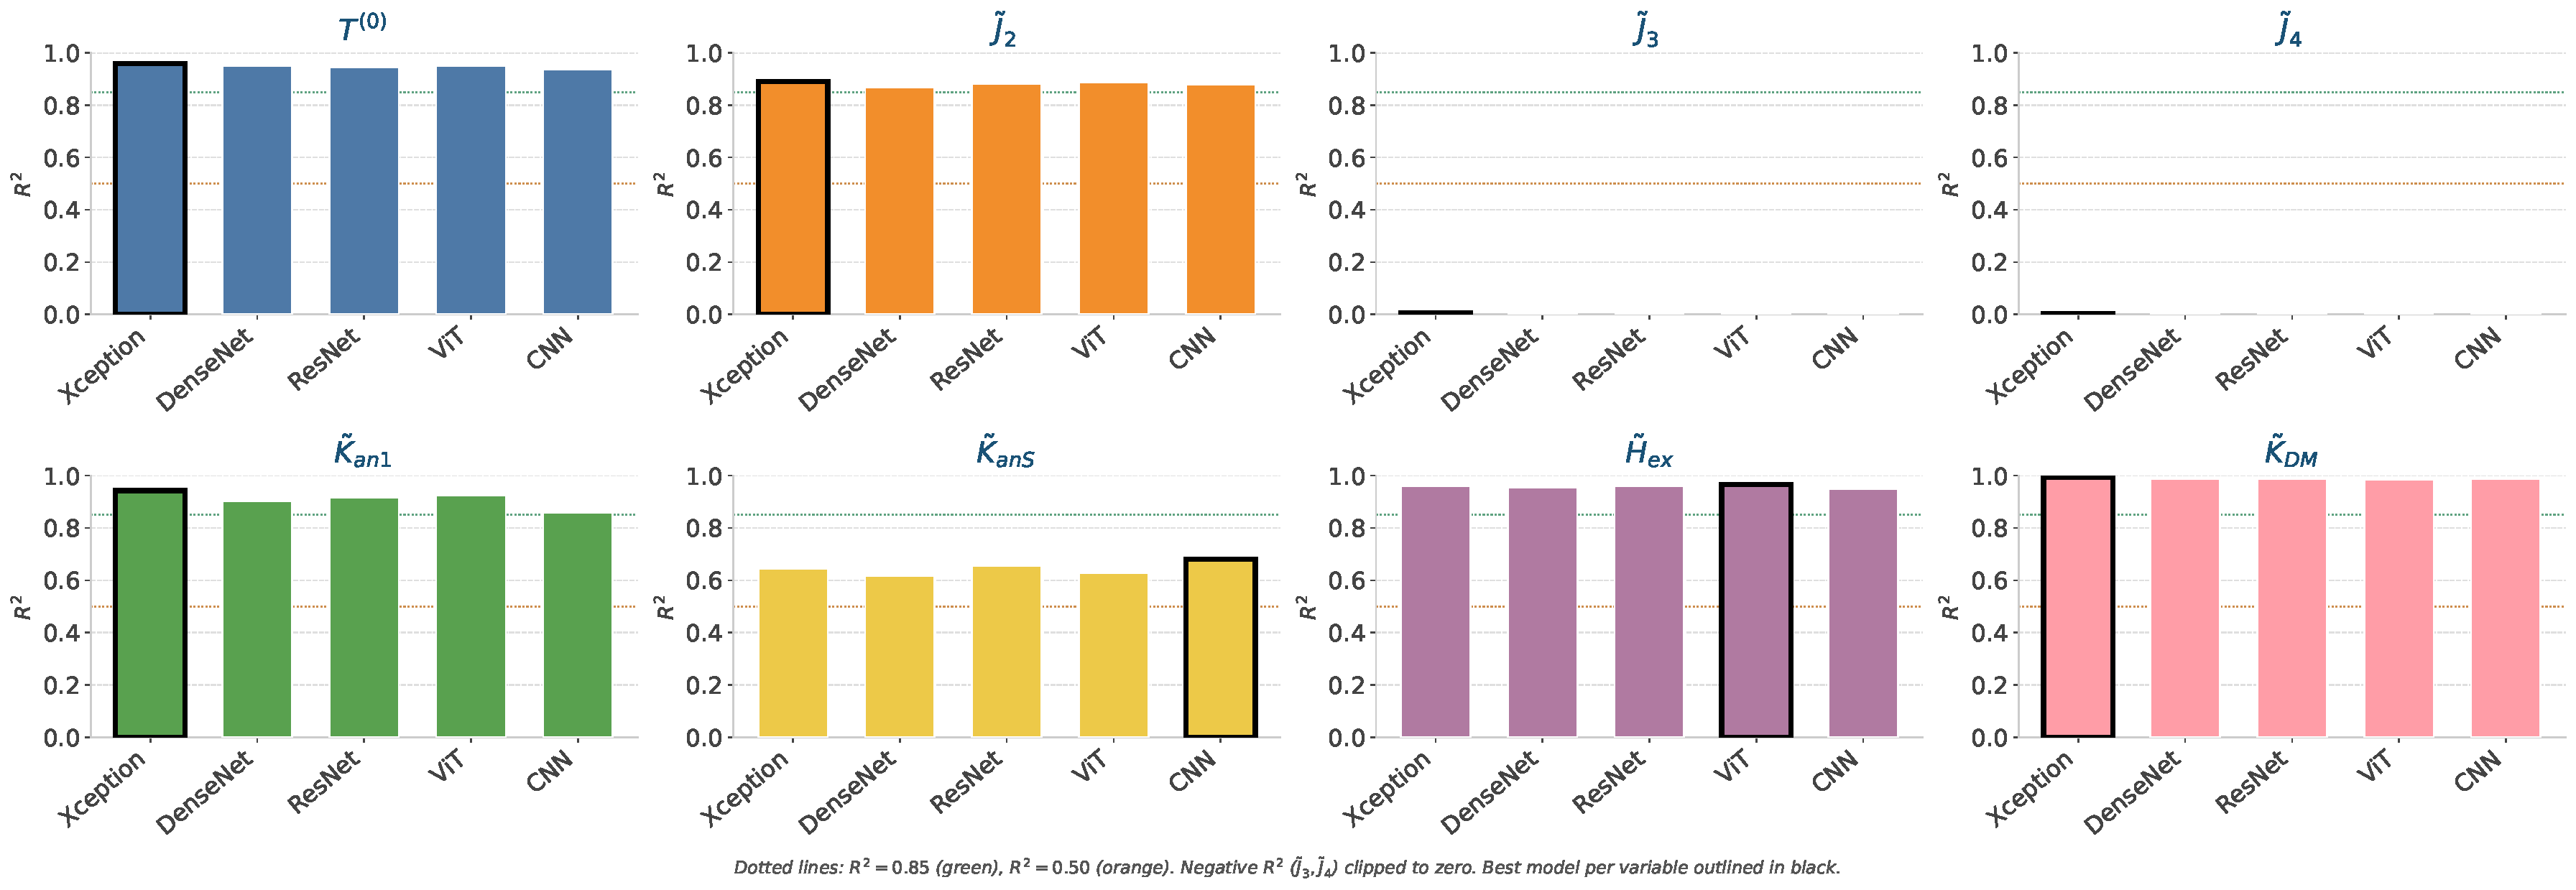
\includegraphics[width=\linewidth]
    {model_comparison_r2-2}
    \caption{Per-variable $R^2$ score across the five evaluated
    architectures (Xception, DenseNet, ResNet, ViT, and the
    conventional CNN baseline) for the eight Hamiltonian parameters
    $\boldsymbol{\theta}$ on the held-out test set. Each panel is one
    parameter, one bar per architecture; negative $R^2$ values are
    clipped to zero, and black-bordered bars mark the best
    architecture per parameter.}
    \label{fig:r2_metrics}
\end{figure*}

\begin{figure*}[!t]
    \centering
    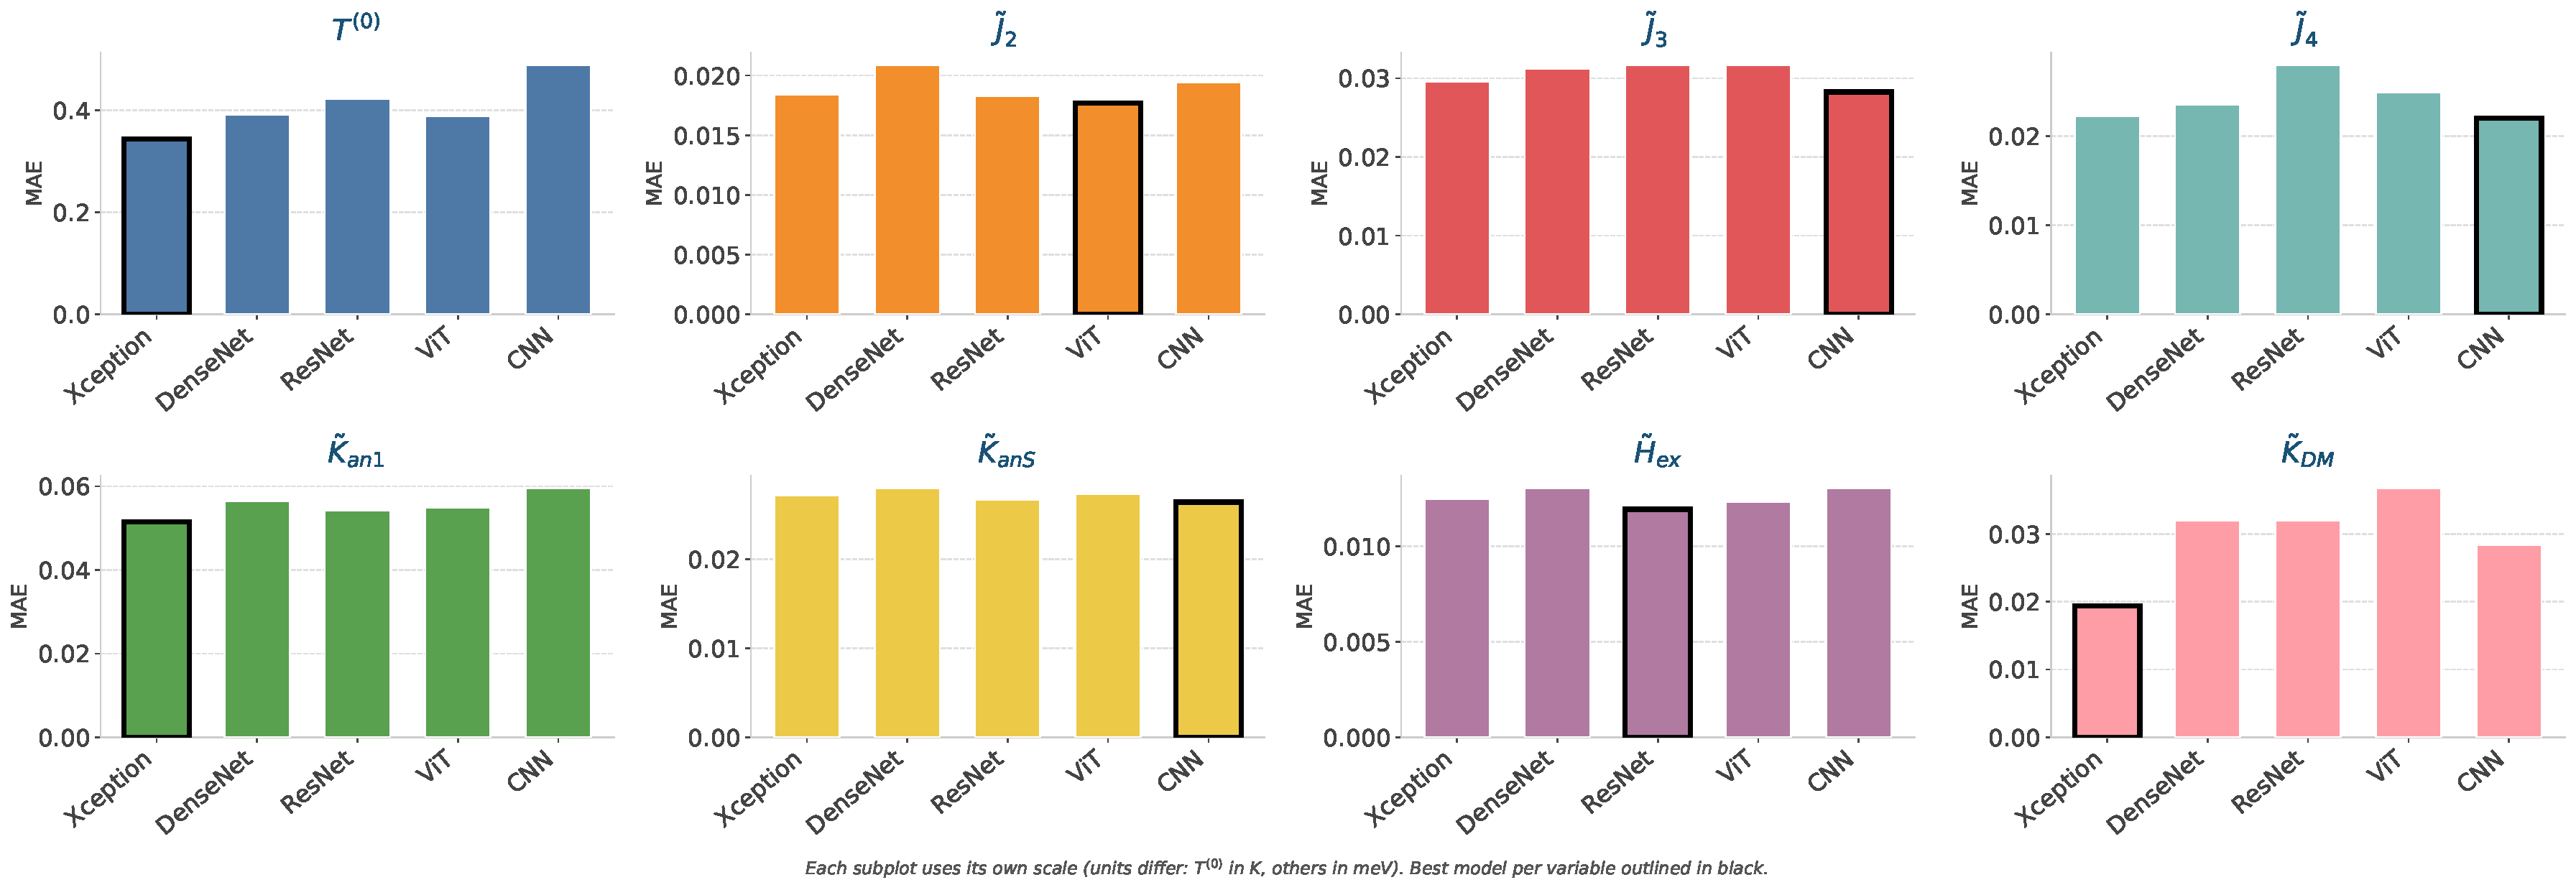
\includegraphics[width=\linewidth]
    {model_comparison_mae-2}
    \caption{Per-variable Mean Absolute Error (MAE) across the five
    evaluated architectures for the eight Hamiltonian parameters
    $\boldsymbol{\theta}$ on the held-out test set, in each
    parameter's physical units (K for $T^{(0)}$, meV for exchange and
    DMI, meV/atom for anisotropy and field). Each panel is one
    parameter, one bar per architecture; black-bordered bars mark the
    best architecture. The small MAE of $\tilde{J}_3$ and
    $\tilde{J}_4$ despite their near-zero $R^2$ reflects their narrow
    dynamic range rather than genuine predictive skill.}
    \label{fig:mae_metrics}
\end{figure*}

%umap visualization
To gain deeper insight into the internal representations learned by
the best-performing model, Xception, during the inverse Hamiltonian estimation task,
Figure~\ref{fig:umap_latent} presents a Uniform Manifold
Approximation and Projection (UMAP) of the model's latent
space~\cite{ghojogh2021uniform}, where each point corresponds to a
test sample colored by the value of each of the eight Hamiltonian
parameters $\boldsymbol{\theta}$. The UMAP embedding was computed
from the high-dimensional feature vectors extracted from the Xception
backbone prior to the regression head, providing a
two-dimensional visualization of the geometric structure that the
model has learned to impose on the magnetization image manifold. 
Rather than forming a single undifferentiated cloud, the latent 
space exhibits a rich topological structure composed of several 
geometrically distinct clusters and continuous gradients, reflecting 
the fact that the model has organized the magnetization textures 
according to their underlying physical regimes. Examining the 
coloring by $T^{(0)}$ reveals the clearest and most spatially 
coherent gradient across the embedding: low-temperature ordered 
configurations concentrate in well-separated compact regions, while 
high-temperature disordered states occupy a large, diffuse cluster 
in the upper portion of the latent space, consistent with the strong 
predictive performance of the model on $T^{(0)}$. The DMI strength 
$\tilde{K}_{DM}$ also produces a structured gradient in the latent 
space, with high-$\tilde{K}_{DM}$ helical configurations forming a 
distinct elongated region separated from the low-$\tilde{K}_{DM}$ 
disordered states, confirming that Xception has successfully encoded
the chiral winding imposed by the DMI as a geometrically meaningful
direction in its latent representation. The bulk anisotropy $\tilde{K}_{an1}$ and the external field
$\tilde{H}_{ex}$ likewise display coherent, structured gradients
across the embedding, mirroring their high regression accuracy and
confirming that Xception encodes them as well-defined directions in
its latent geometry --- a direct consequence of the out-of-plane
field configurations and the extended anisotropy range, which render
these parameters observable in the $s_z$ projection. In contrast, the
longer-range exchange constants $\tilde{J}_3$ and $\tilde{J}_4$
produce nearly uniform colorings across the entire embedding,
indicating that the model's internal representations carry little
discriminative information about these parameters --- a result that
is fully consistent with their low $R^2$ values and their energetic
subordination to the dominant first-shell exchange
$\tilde{J}_1 = 1.0$~meV. The surface anisotropy $\tilde{K}_{anS}$
occupies an intermediate case, showing a partially mixed coloring
consistent with its moderate identifiability and its entanglement
with the bulk anisotropy signature.

%umap 2D
Beyond the per-parameter gradients, the same embedding reveals that
Xception has organized the magnetization textures into geometrically
distinct and physically interpretable regions, without any explicit
supervision of magnetic phase labels. The systematic variation of
$T^{(0)}$ separates ordered, low-temperature configurations---which
concentrate in compact, well-separated regions---from the thermally
disordered states that occupy a large, diffuse cluster at high
$T^{(0)}$, where thermal fluctuations dominate over the competing
energetic contributions of $\tilde{J}_1$ and $\tilde{K}_{DM}$.
Superimposed on this temperature axis, the $\tilde{K}_{DM}$ gradient
further resolves the ordered region into the chiral helical, dense
skyrmionic, and collinear Ising-like regimes, while the mixed-chirality
configurations form their own transitional zone. This spontaneous
geometric separation motivates a structured clustering analysis,
performed directly on the two-dimensional UMAP embedding of the test
set feature vectors (min-max normalized to $[0,1]$ along each axis),
which we use next to identify and characterize the dominant magnetic
phases.

%UMAP Xception
\begin{figure*}[!t]
    \centering
    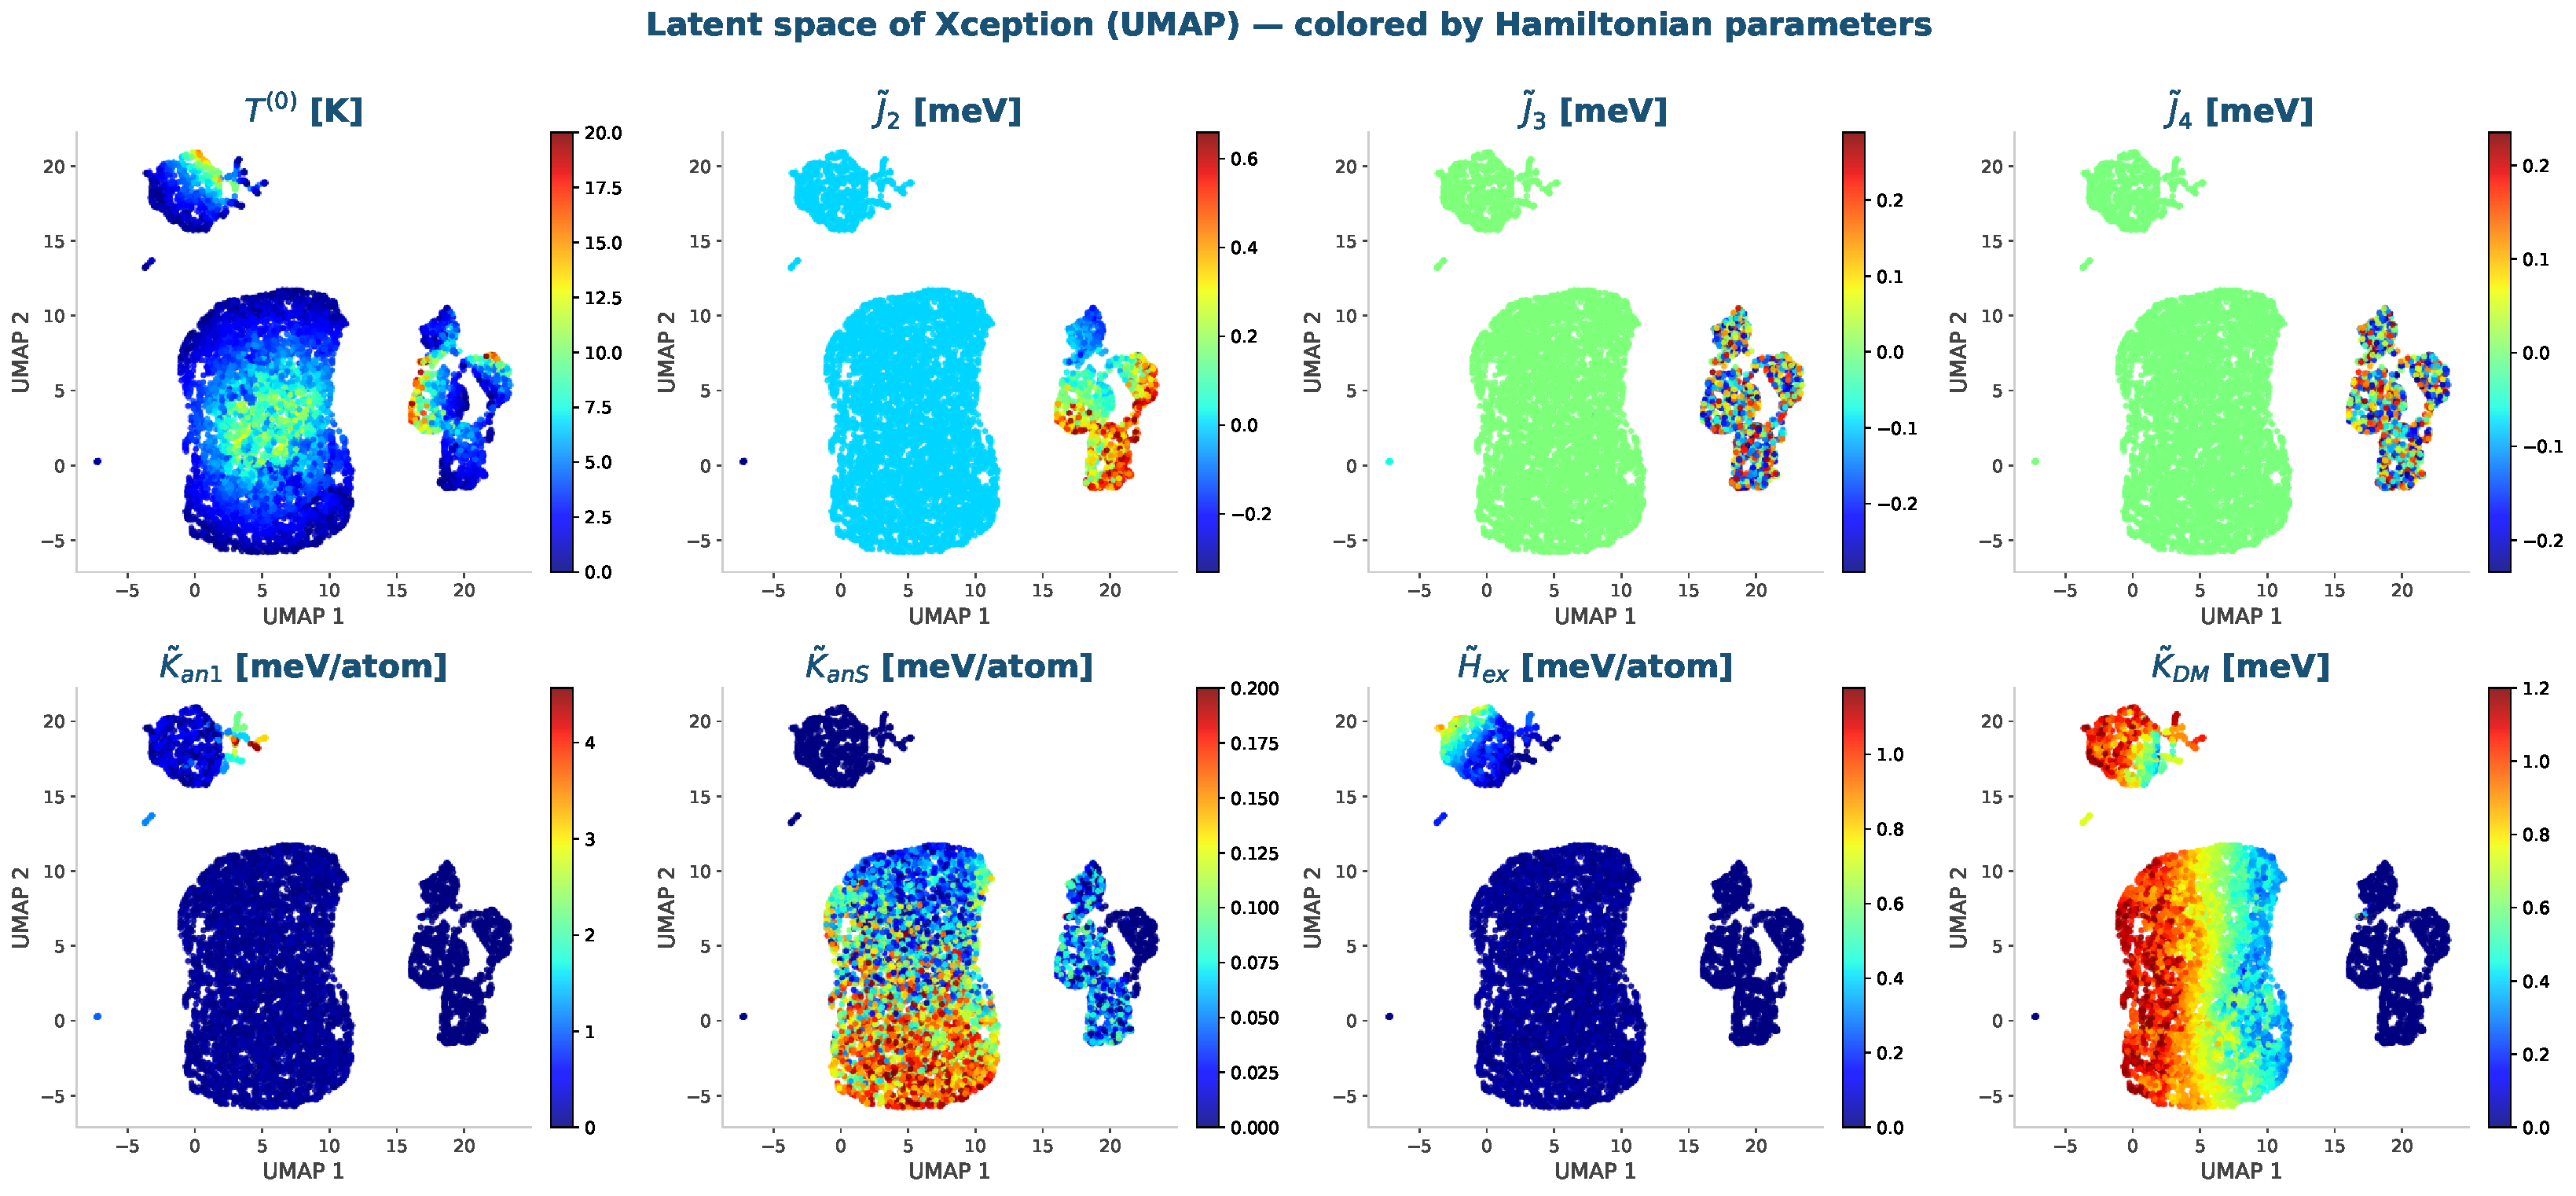
\includegraphics[width=\linewidth, trim=0 0 0 43.8bp, clip]
    {latent_xception_umap}
    \caption{UMAP-based 2D projection of the Xception latent space
    on the held-out test set, colored by each of the eight
    Hamiltonian parameters $\boldsymbol{\theta} = [T^{(0)},
    \tilde{J}_2, \tilde{J}_3, \tilde{J}_4, \tilde{K}_{an1},
    \tilde{K}_{anS}, \tilde{H}_{ex}, \tilde{K}_{DM}]$. Each
    point represents a magnetization image $\mathbf{X}_n$
    projected from the high-dimensional feature space of the
    Xception backbone into two dimensions via UMAP.}
    \label{fig:umap_latent}
\end{figure*}


To systematically identify and characterize the dominant magnetic
phases encoded in the latent space, a density-based clustering
analysis was performed using the HDBSCAN algorithm on the UMAP
embedding, followed by a KMeans subdivision of anomalously large
clusters. Based on visual inspection of representative samples
and the mean values of the Hamiltonian parameters
$\boldsymbol{\theta}$ within each group, the resulting clusters
were consolidated into five physically meaningful magnetic phase
categories.

The \textit{helical phase} contains the most spatially coherent and regularly ordered configurations in the dataset, displaying well-defined stripe and labyrinthine patterns with consistent chiral winding direction and spatial periodicity across the nanodot, stabilized at low annealing temperature by a moderate DMI ($\langle\tilde{K}_{DM}\rangle \approx 0.75$~meV). The \textit{skyrmion phase} groups configurations in which the strong DMI ($\langle\tilde{K}_{DM}\rangle \approx 0.88$~meV) stabilizes dense lattices of isolated, radially symmetric topological solitons, clearly visible as arrays of circular cores of reversed $s_z$ embedded in a uniform background. The \textit{Ising phase} comprises the low-temperature ($\langle T^{(0)}\rangle \approx 1.86$~K), high-anisotropy configurations characterized by sharp, discrete domain walls separating collinear up/down regions, reflecting the deliberately extended anisotropy range that drives the system toward an Ising-like regime. The \textit{bimeron phase} gathers mixed-chirality textures in which in-plane and out-of-plane components coexist as paired meron-antimeron structures, forming irregular large-scale domains without the long-range periodicity of the helical phase. Finally, the \textit{others} category constitutes the most heterogeneous group, gathering thermally disordered states in which thermal fluctuations have disrupted long-range spin order, transitional configurations located at the boundaries between competing phases, and topologically mixed textures whose spatial structure is ambiguous. The common characteristic of this group is the absence of a distinctive and reproducible magnetization pattern, making them the most structurally ill-conditioned samples in the dataset.

Figure~\ref{fig:structure_representatives} presents five
representative magnetization images per phase, selected as the
samples closest to the centroid of each group in the UMAP
embedding, along with the mean Hamiltonian parameters
$\langle T^{(0)}\rangle$, $\langle\tilde{J}_2\rangle$, and
$\langle\tilde{K}_{DM}\rangle$ characterizing each phase.

\begin{figure*}[!t]
    \centering
    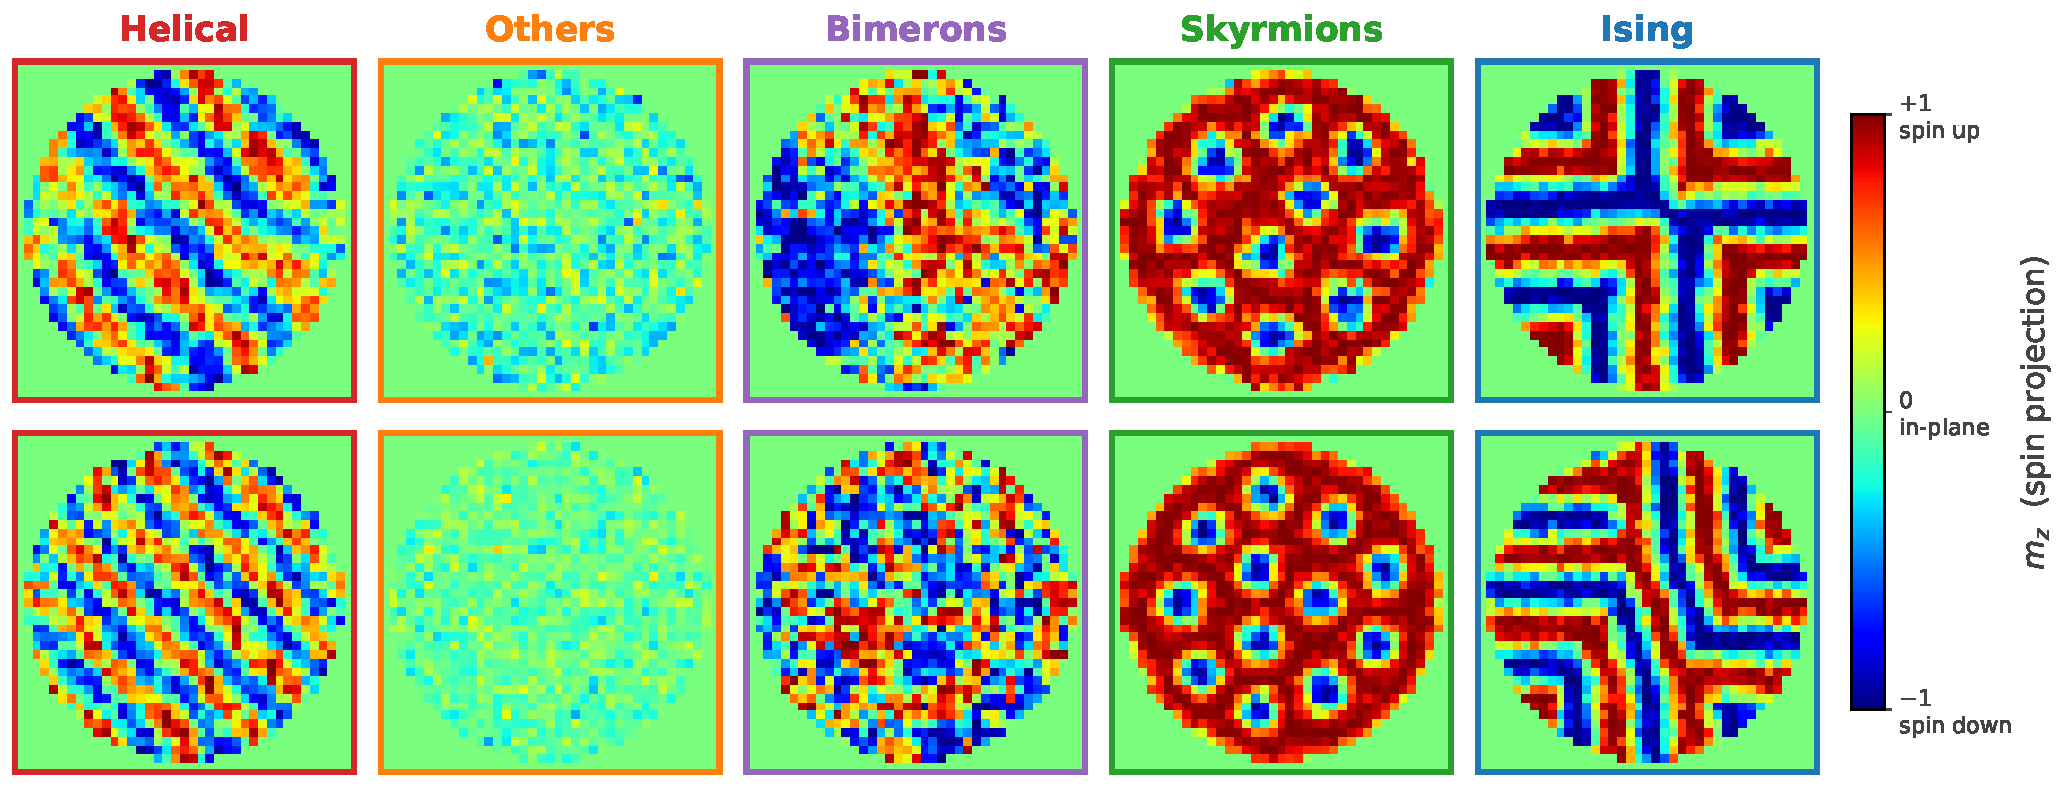
\includegraphics[width=0.75\linewidth]
    {structures_representatives_horizontal}
    \caption{Representative magnetization images $\mathbf{X}_n$ for
    the five magnetic phase categories identified by clustering the
    Xception latent space. Each column is one phase (two samples
    nearest the cluster centroid in the UMAP embedding); color
    encodes the out-of-plane component $m_z$ ($+1$ spin up, $-1$ spin
    down). The phases span ordered helical stripes, thermally
    disordered \textit{others}, mixed-chirality bimerons, dense
    skyrmion lattices, and sharp Ising domain walls.}
    \label{fig:structure_representatives}
\end{figure*}

The per-phase regression performance of the best-performing model,
Xception, is summarized in Figures~\ref{fig:metrics_by_structure}
and~\ref{fig:mae_by_structure}. The results reveal a pronounced
heterogeneity in predictive accuracy across magnetic phases that
is physically consistent with the identifiability analysis
presented earlier in this section. The \textit{skyrmion} and
\textit{Ising} phases achieve the highest $R^2$ values (typically
$0.94$--$0.99$) and the lowest MAE across essentially all
identifiable parameters, reflecting the fact that these highly
ordered configurations---dense soliton lattices and sharp,
discrete domain walls, respectively---exhibit the most
discriminative and spatially coherent signatures in the $s_z$
projection. Within these phases, the well-defined periodicity and
topological structure of the magnetization texture provide
unambiguous observational constraints that allow the model to
recover the underlying Hamiltonian parameters with high fidelity.
The \textit{helical} phase follows closely, with excellent recovery
of $T^{(0)}$ and $\tilde{K}_{DM}$ ($R^2 \approx 0.99$) and good
performance for $\tilde{J}_2$ and $\tilde{H}_{ex}$, although its
anisotropy constants are estimated less accurately owing to the
weaker anisotropic imprint in the chiral stripe regime.

\begin{figure}[t]
    \centering
    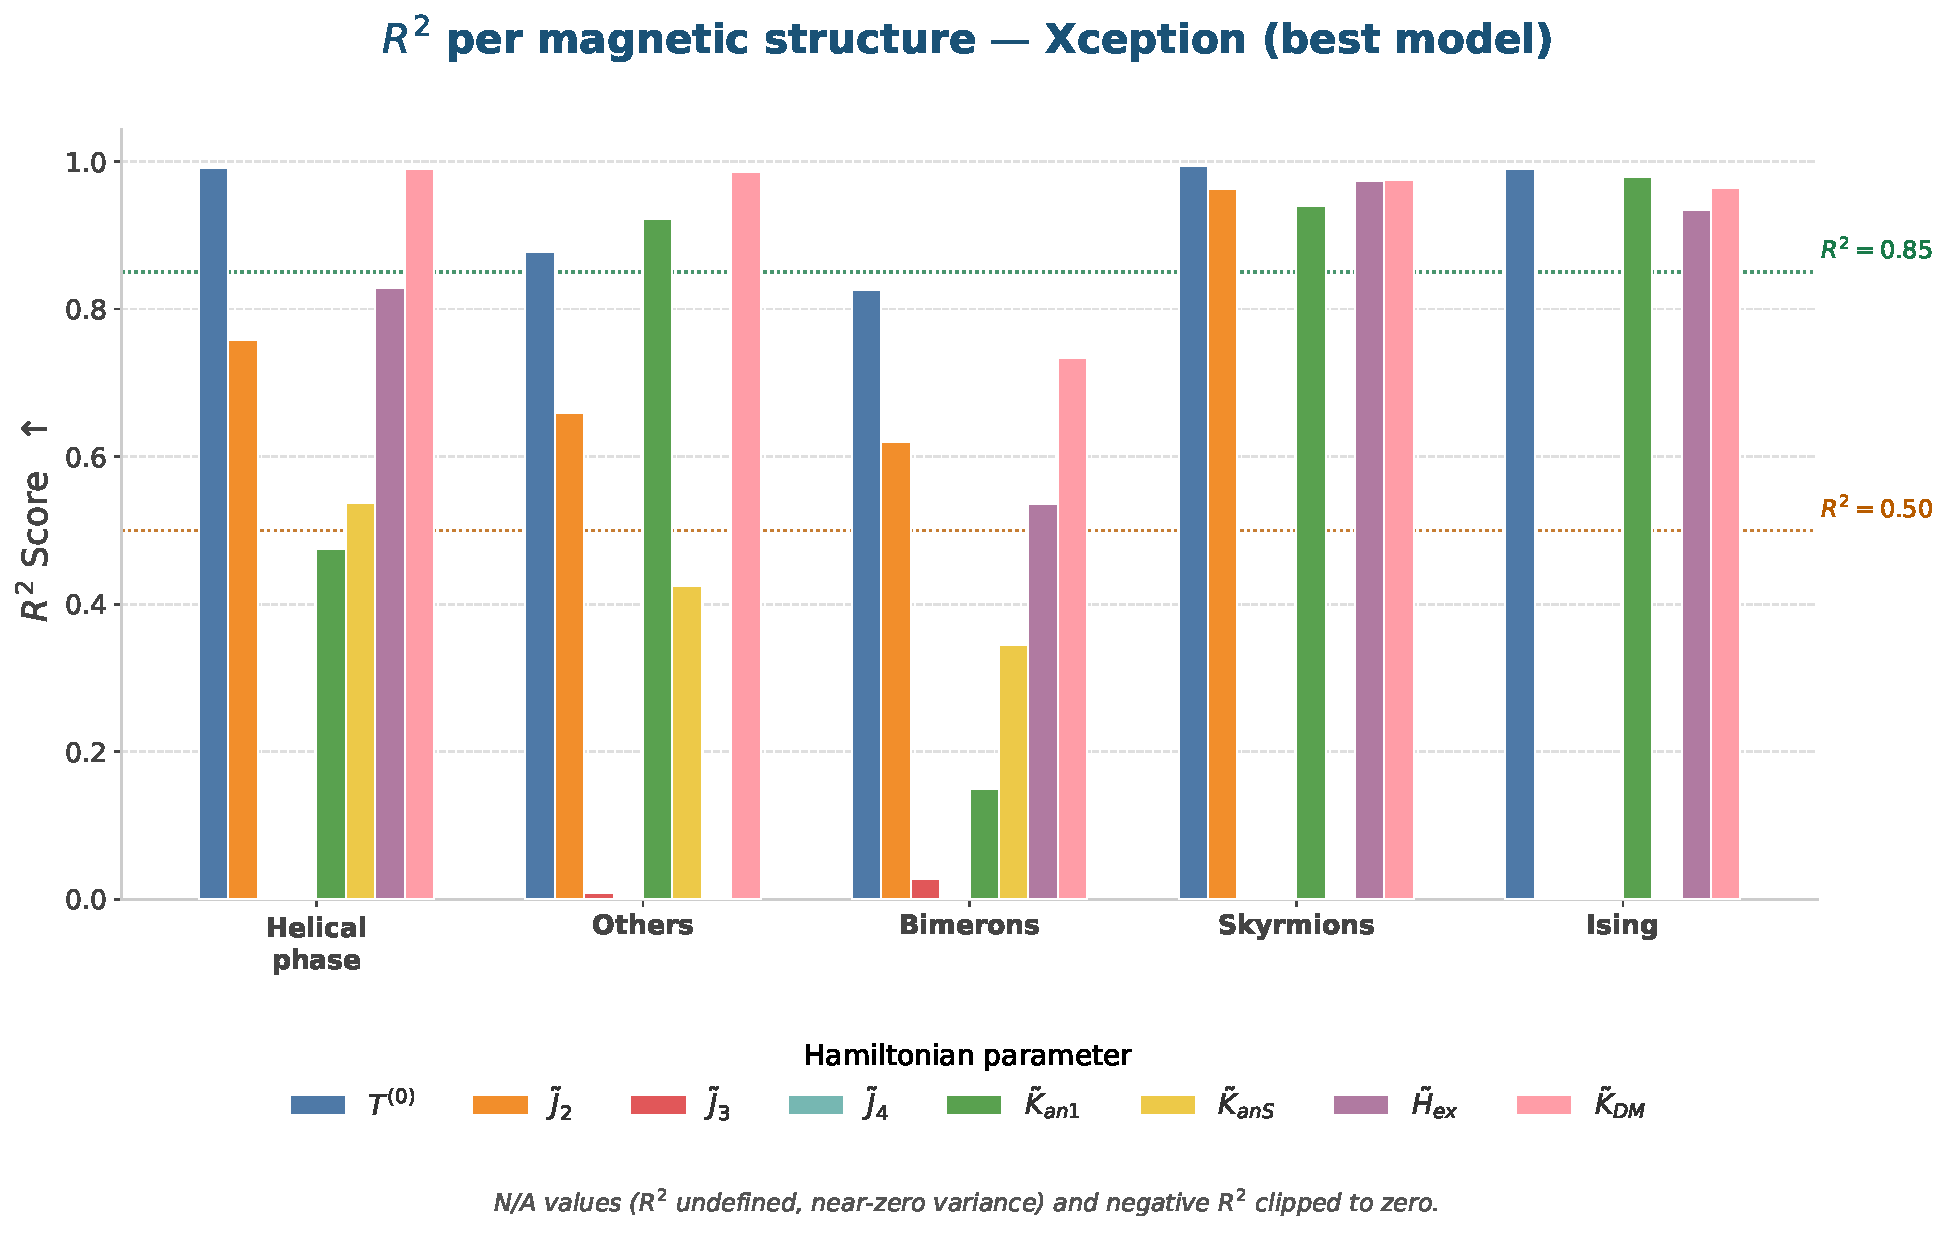
\includegraphics[width=\linewidth, keepaspectratio, trim=0 0 0 41.4bp, clip]
    {metrics_by_structure_r2}
    \caption{Per-phase $R^2$ score of Xception across the eight
    Hamiltonian parameters $\boldsymbol{\theta}$ for the five magnetic
    phases. Each bar group is one phase, each bar one parameter;
    dashed lines mark the $R^2 = 0.85$ (high) and $R^2 = 0.50$
    (partial) predictability thresholds, and negative or
    near-zero-variance cases (N/A) are clipped to zero.}
    \label{fig:metrics_by_structure}
\end{figure}

In stark contrast, the \textit{others} and \textit{bimeron}
categories concentrate the largest absolute errors across
virtually all Hamiltonian parameters, as evidenced by the dominant
MAE values in Figure~\ref{fig:mae_by_structure}. This result
directly confirms the physical interpretation advanced earlier:
the thermally disordered configurations grouped in the
\textit{others} category, and the mixed-chirality meron-antimeron
textures of the \textit{bimeron} phase, relax into structurally
weakly-discriminative magnetization patterns, so that widely
different parameter combinations produce statistically similar
textures and inflate the inverse-mapping error within these
regimes. The elevated MAE for $T^{(0)}$ in the \textit{others}
phase is particularly revealing, as it quantitatively isolates the
contribution of the high-temperature paramagnetic regime to the
global prediction error observed in the aggregated analysis;
likewise, the \textit{bimeron} phase yields the lowest $R^2$ for
the anisotropy and field parameters, reflecting the intrinsic
spatial ambiguity of its coexisting in-plane and out-of-plane
components.

Across all five phases, the higher-order exchange constants
$\tilde{J}_3$ and $\tilde{J}_4$ retain near-zero $R^2$, confirming
at the per-phase level that their unidentifiability is a
fundamental property of the $s_z$ observation rather than an
artifact of any particular structural regime.

\begin{figure*}[!t]
    \centering
    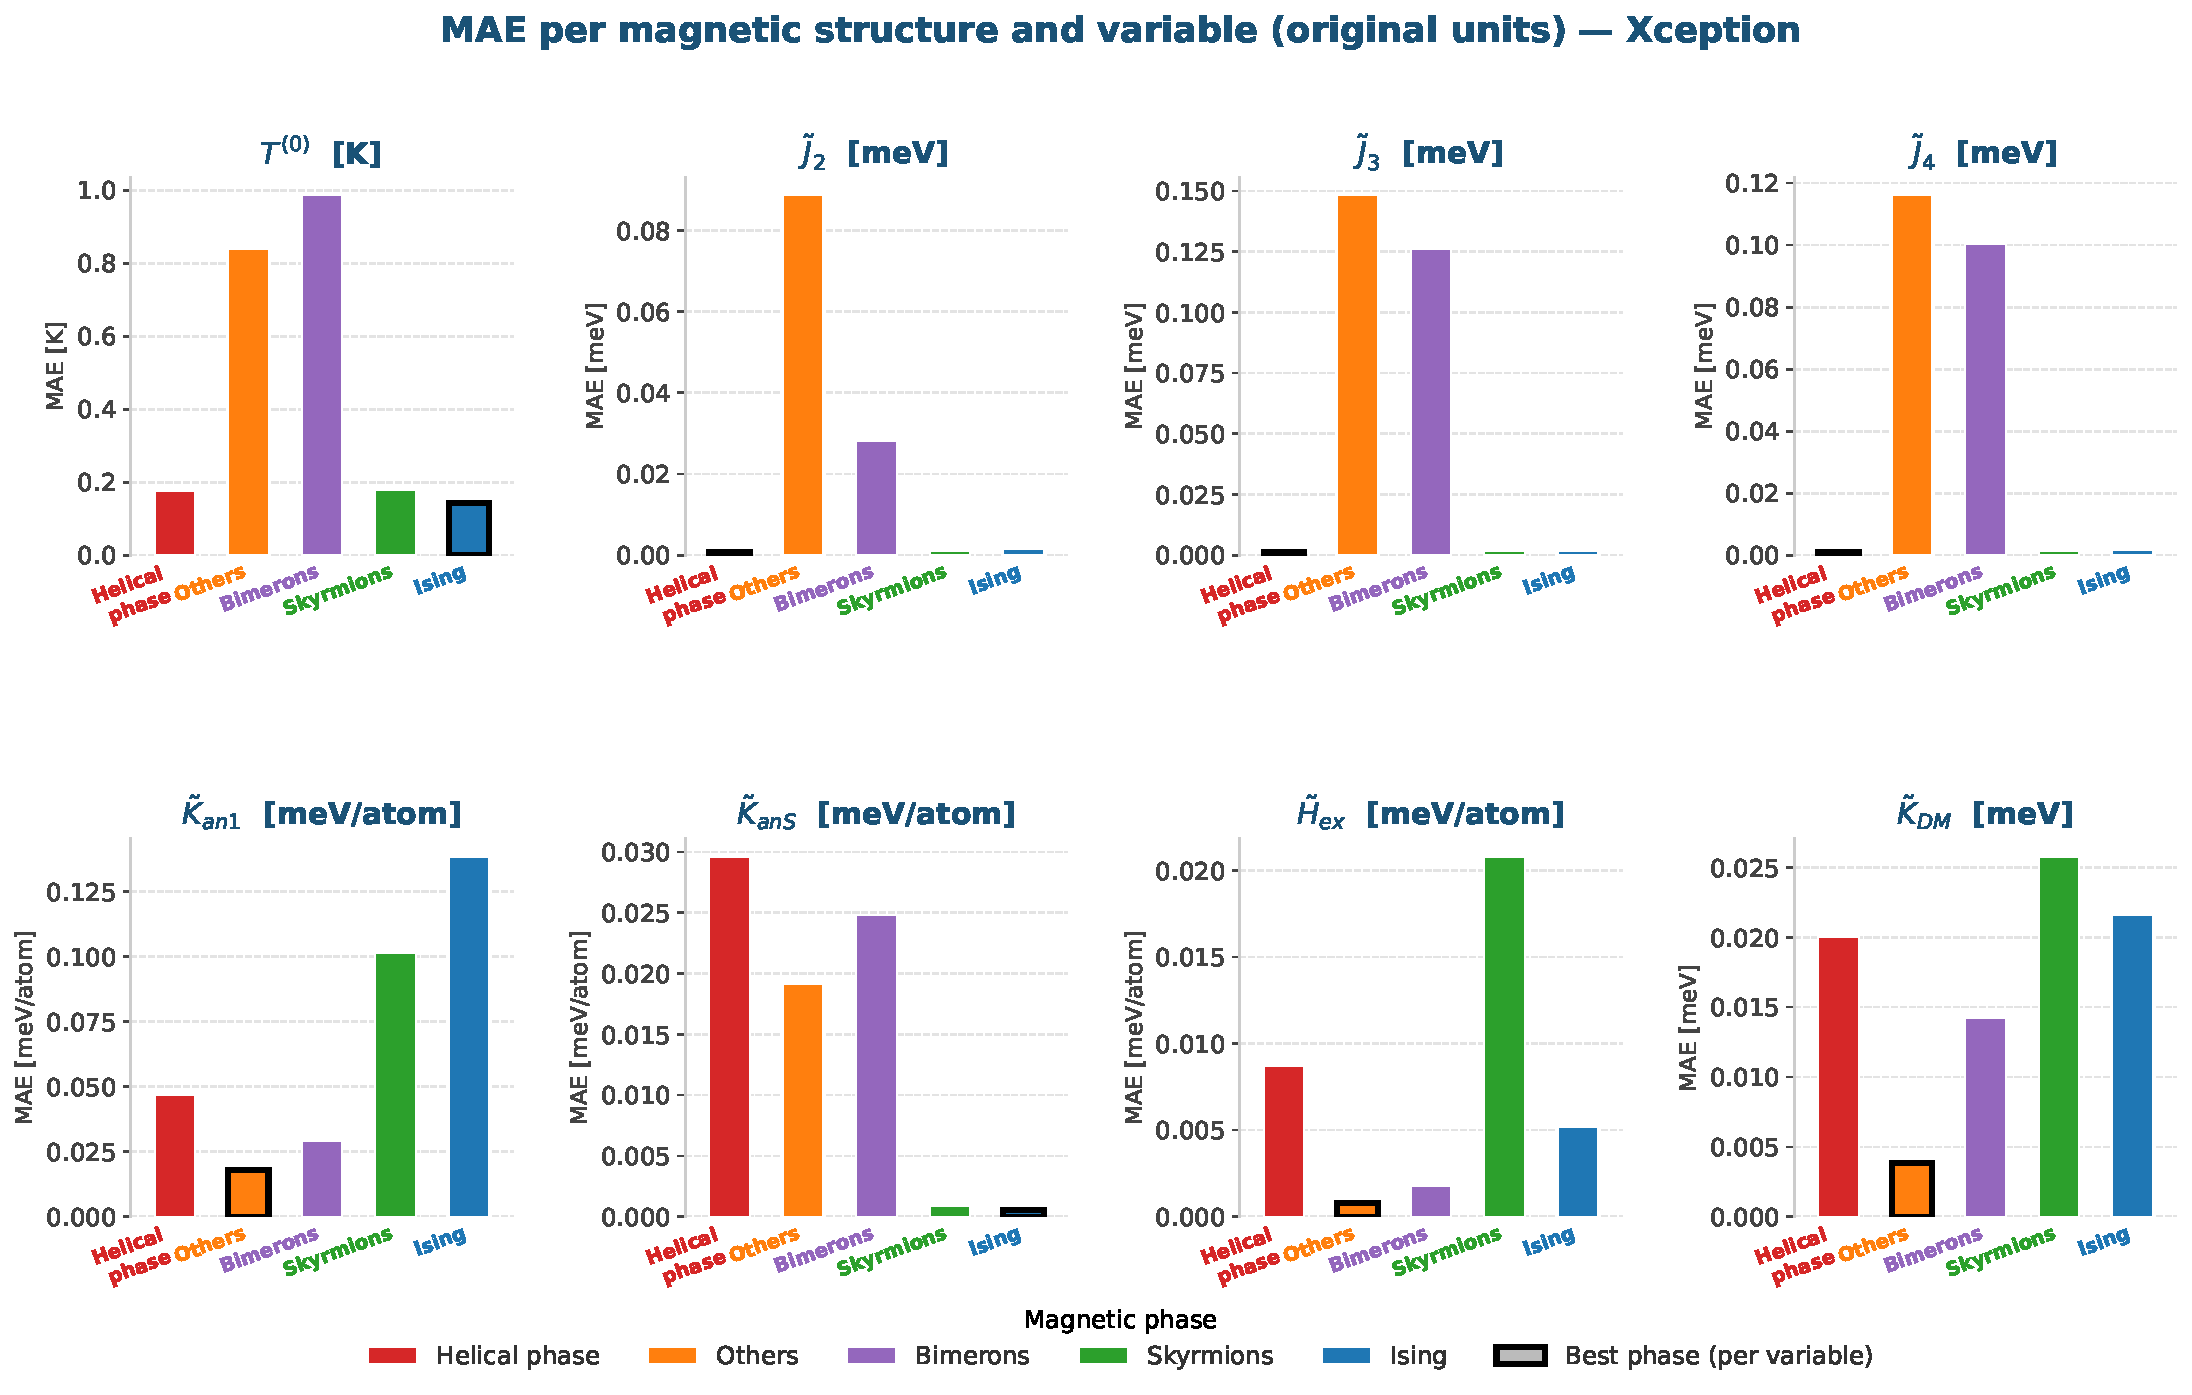
\includegraphics[width=\linewidth, keepaspectratio, trim=0 0 0 33.5bp, clip]
    {metrics_by_structure_mae_grid}
    \caption{Per-phase Mean Absolute Error (MAE) of Xception across
    the eight Hamiltonian parameters $\boldsymbol{\theta}$ for the
    five magnetic phases, in each parameter's physical units. Each
    panel is one parameter, one bar per phase; black-bordered bars
    mark the phase with the lowest MAE. The \textit{others} and
    \textit{bimeron} categories concentrate the largest errors across
    most parameters.}
    \label{fig:mae_by_structure}
\end{figure*}

\subsection{RAMs-based Interpretability Results}
\label{sec:rams_results}

%\subsubsection{Spatial Interpretability via Xception}
To spatially trace the predictive behavior of the Xception
architecture across the identified magnetic phase categories,
RAMs were computed following the
CNN-based formulation introduced in
Section~\ref{sec:CNN_RAMs}. For each of the five magnetic
phases a single representative magnetization image
$\mathbf{X}_n$ was selected as the sample closest to the
centroid of the corresponding cluster group in the UMAP
latent space, maximizing the concentration of gradient
activations within the physical extent of the nanodot disk.
For the spatial overlays, RAMs were computed for three
representative Hamiltonian parameters ($T^{(0)}$, $\tilde{J}_2$,
and $\tilde{K}_{DM}$) across eight strategically selected
convolutional layers of the Xception backbone, spanning the
full depth of the network:

\begin{itemize}
    \item[--] \texttt{block1\_conv2}: entry-level features
    at spatial resolution $112\times112$, capturing
    low-level pixel-scale magnetization gradients.
    \item[--] \texttt{block3\_sepconv2} and
    \texttt{block4\_sepconv2}: intermediate entry-flow
    layers at $56\times56$ and $28\times28$, encoding
    domain boundary frequencies and local spin-winding
    patterns.
    \item[--] \texttt{block6\_sepconv2} through
    \texttt{block12\_sepconv2}: middle-flow layers at
    $14\times14$, constituting the deepest repeated
    processing stage of Xception and encoding progressively
    more abstract topological representations of the
    magnetic texture.
    \item[--] \texttt{block13\_sepconv2}: exit-flow
    transition layer prior to global pooling, encoding
    high-level semantic representations of the global
    magnetic phase.
\end{itemize}

\paragraph{Selection of the precision factor $\gamma$.}
The precision factor $\gamma$ in the RAM objective
$\mathcal{O}_p = \exp\!\left(-\gamma\left(\theta_p -
\hat{\theta}_p\right)^2\right)$ governs the selectivity
of the gradient signal: small values render the objective
nearly constant regardless of prediction quality, producing
spatially uninformative maps, while excessively large values
collapse the gradient to zero for parameters with
non-negligible prediction error, yielding empty activation
maps. To select $\gamma$ in a principled and data-driven
manner, a sensitivity analysis was conducted by evaluating
the objective $\mathcal{O}_p$ at the empirical mean
prediction error $\bar{\varepsilon}_p =
\langle|\theta_p - \hat{\theta}_p|\rangle$ of each
Hamiltonian parameter on the test set, for values spanning
$\gamma \in \{0.1, 0.3, 0.5, 1, 2, 5, 10, 20, 50, 100\}$.

Figure~\ref{fig:gamma_selection} illustrates the resulting
sensitivity curves. The left panel shows the shape of the
Gaussian objective as a function of the prediction error
$\varepsilon$ for each candidate $\gamma$: values below
$\gamma = 1$ produce flat curves that activate almost
uniformly regardless of prediction quality, while values
above $\gamma = 20$ generate overly steep curves that
suppress the gradient for errors as small as $\varepsilon
\approx 0.2$; the selected $\gamma = 10$ provides an
intermediate, well-graded response. The right panel
evaluates $\mathcal{O}_p$ at the empirical mean error of
each parameter as a function of $\gamma$: because the
identifiable parameters ($T^{(0)}$, $\tilde{J}_2$, and
$\tilde{K}_{DM}$) are recovered with small mean errors,
their objective remains close to unity across the entire
$\gamma$ range and never approaches the gradient collapse
threshold $\mathcal{O}_p < 0.05$. Only the poorly identified
higher-order exchange constant $\tilde{J}_3$, whose mean
error is comparatively large, shows a noticeable decline at
high $\gamma$ (down to $\mathcal{O}_p \approx 0.8$ at
$\gamma = 100$), yet even it stays well above the collapse
regime. The value $\gamma = 10$ was therefore selected as
the operating point: it is selective enough to yield
spatially discriminative maps (steep left-panel response)
while keeping a well-conditioned gradient signal for all
Hamiltonian parameters.

\begin{figure*}[!t]
    \centering
    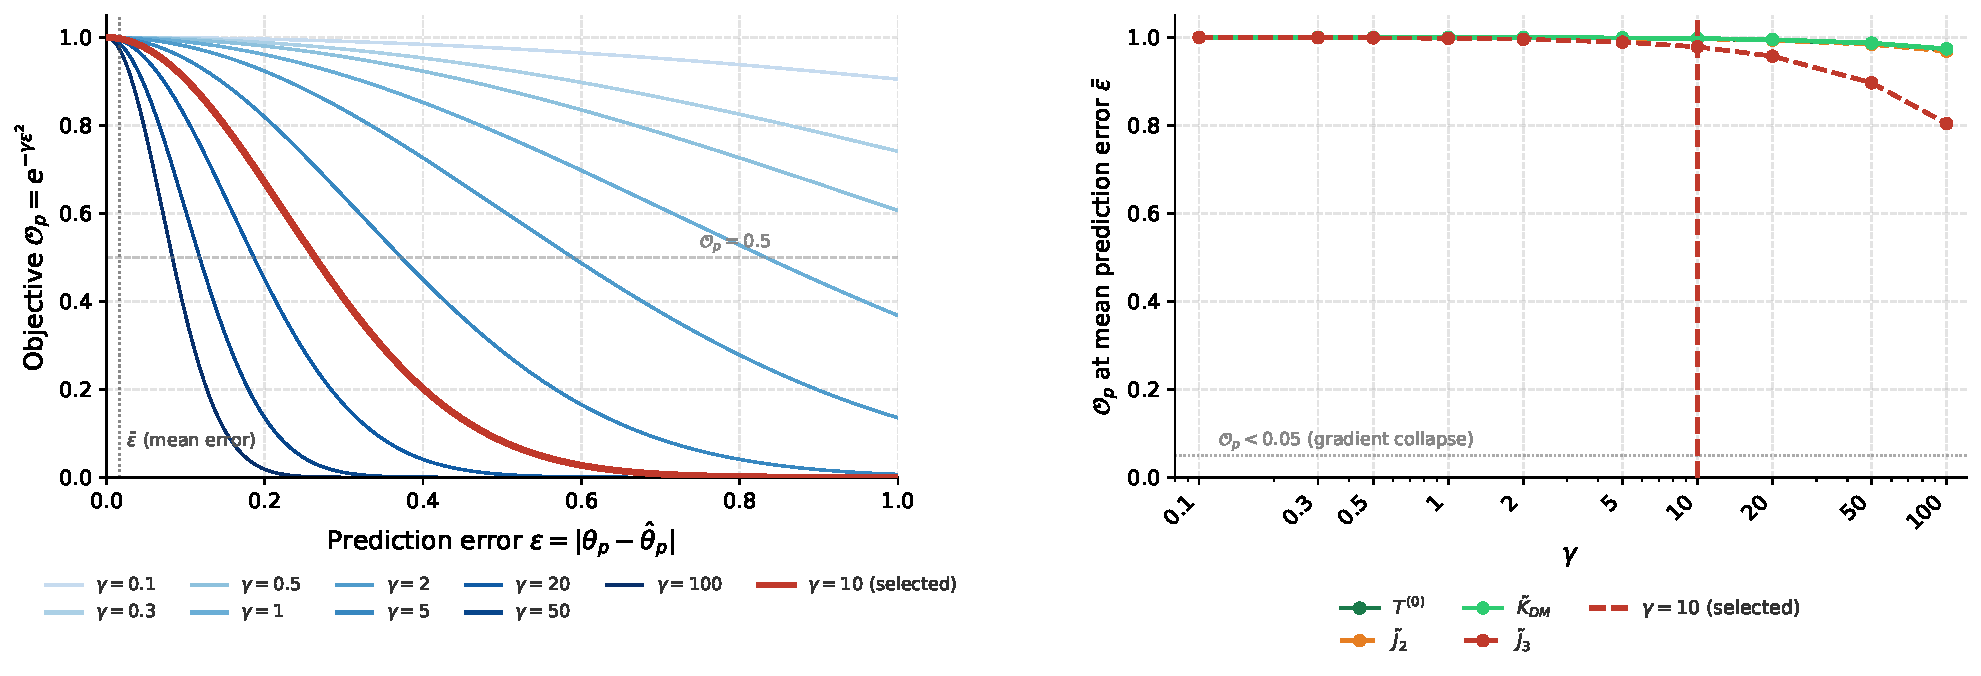
\includegraphics[width=\linewidth, keepaspectratio]
    {gamma_gaussian_shape-2}
    \caption{Sensitivity analysis of the RAM precision factor
    $\gamma$. Left: shape of the Gaussian objective
    $\mathcal{O}_p = e^{-\gamma\varepsilon^2}$ versus the prediction
    error $\varepsilon = |\theta_p - \hat{\theta}_p|$ for
    $\gamma \in \{0.1, \dots, 100\}$ (selected $\gamma = 10$ in red;
    vertical dotted line = empirical mean error). Right:
    $\mathcal{O}_p$ evaluated at each parameter's mean error as a
    function of $\gamma$; the horizontal dotted line marks the
    gradient-collapse threshold $\mathcal{O}_p = 0.05$. The value
    $\gamma = 10$ is the selected operating point.}
    \label{fig:gamma_selection}
\end{figure*}

To ensure that activation magnitudes remain physically
interpretable and spatially confined to the nanodot
geometry, each RAM was masked by a circular binary mask
aligned with the disk boundary prior to normalization.
The globally normalized RAMs
$\tilde{\mathcal{R}}_{\text{RAM}}^{(l,p)}$ were obtained
following Equation~\ref{eq:RAM_Global_Norm}, and the
spatial patterns were additionally visualized under local
per-cell normalization to reveal the gradient attribution
structure at each individual layer.

Figure~\ref{fig:rams_xception_unified} presents the
resulting RAM overlays for the skyrmion phase, selected for
visualization because its dense lattice of isolated,
radially symmetric solitons produces the clearest and most
physically interpretable gradient attribution patterns,
providing the strongest validation of the hierarchical
decoupling hypothesis. The spatial attribution patterns
reveal a physically consistent progression across network
depth. In the early entry-flow layers
(\texttt{block1\_conv2}, \texttt{block3\_sepconv2}), the
activations for $\tilde{K}_{DM}$ are spatially dense and
sharply structured, coinciding with the individual skyrmion
cores and their boundaries --- precisely the chiral features
that encode the DMI strength. As depth increases through the
middle-flow layers (\texttt{block6} through
\texttt{block12}), these activations progressively
consolidate into coarser, spatially localized hotspots
centered on the topologically significant skyrmion cores,
while the $T^{(0)}$ attribution spreads over the inter-core
background that reflects the global degree of thermal order.
In the terminal exit-flow layer (\texttt{block13\_sepconv2}),
activations become concentrated in a small number of compact
regions, indicating that the network's final semantic
representations encode global topological stability rather
than local texture periodicity. Consistently, the
$\tilde{J}_2$ row remains nearly inactive across all layers,
in agreement with its vanishing value in this phase. This
hierarchical progression matches the theoretical prediction
of Section~\ref{sec:Nor_RAMs}: early layers resolve the
short-range energetic competition between $\tilde{J}_1$ and
$\tilde{K}_{DM}$, while deeper layers integrate these local
features into macro-scale thermodynamic representations
governed by $T^{(0)}$.

\begin{figure*}[!t]
    \centering
    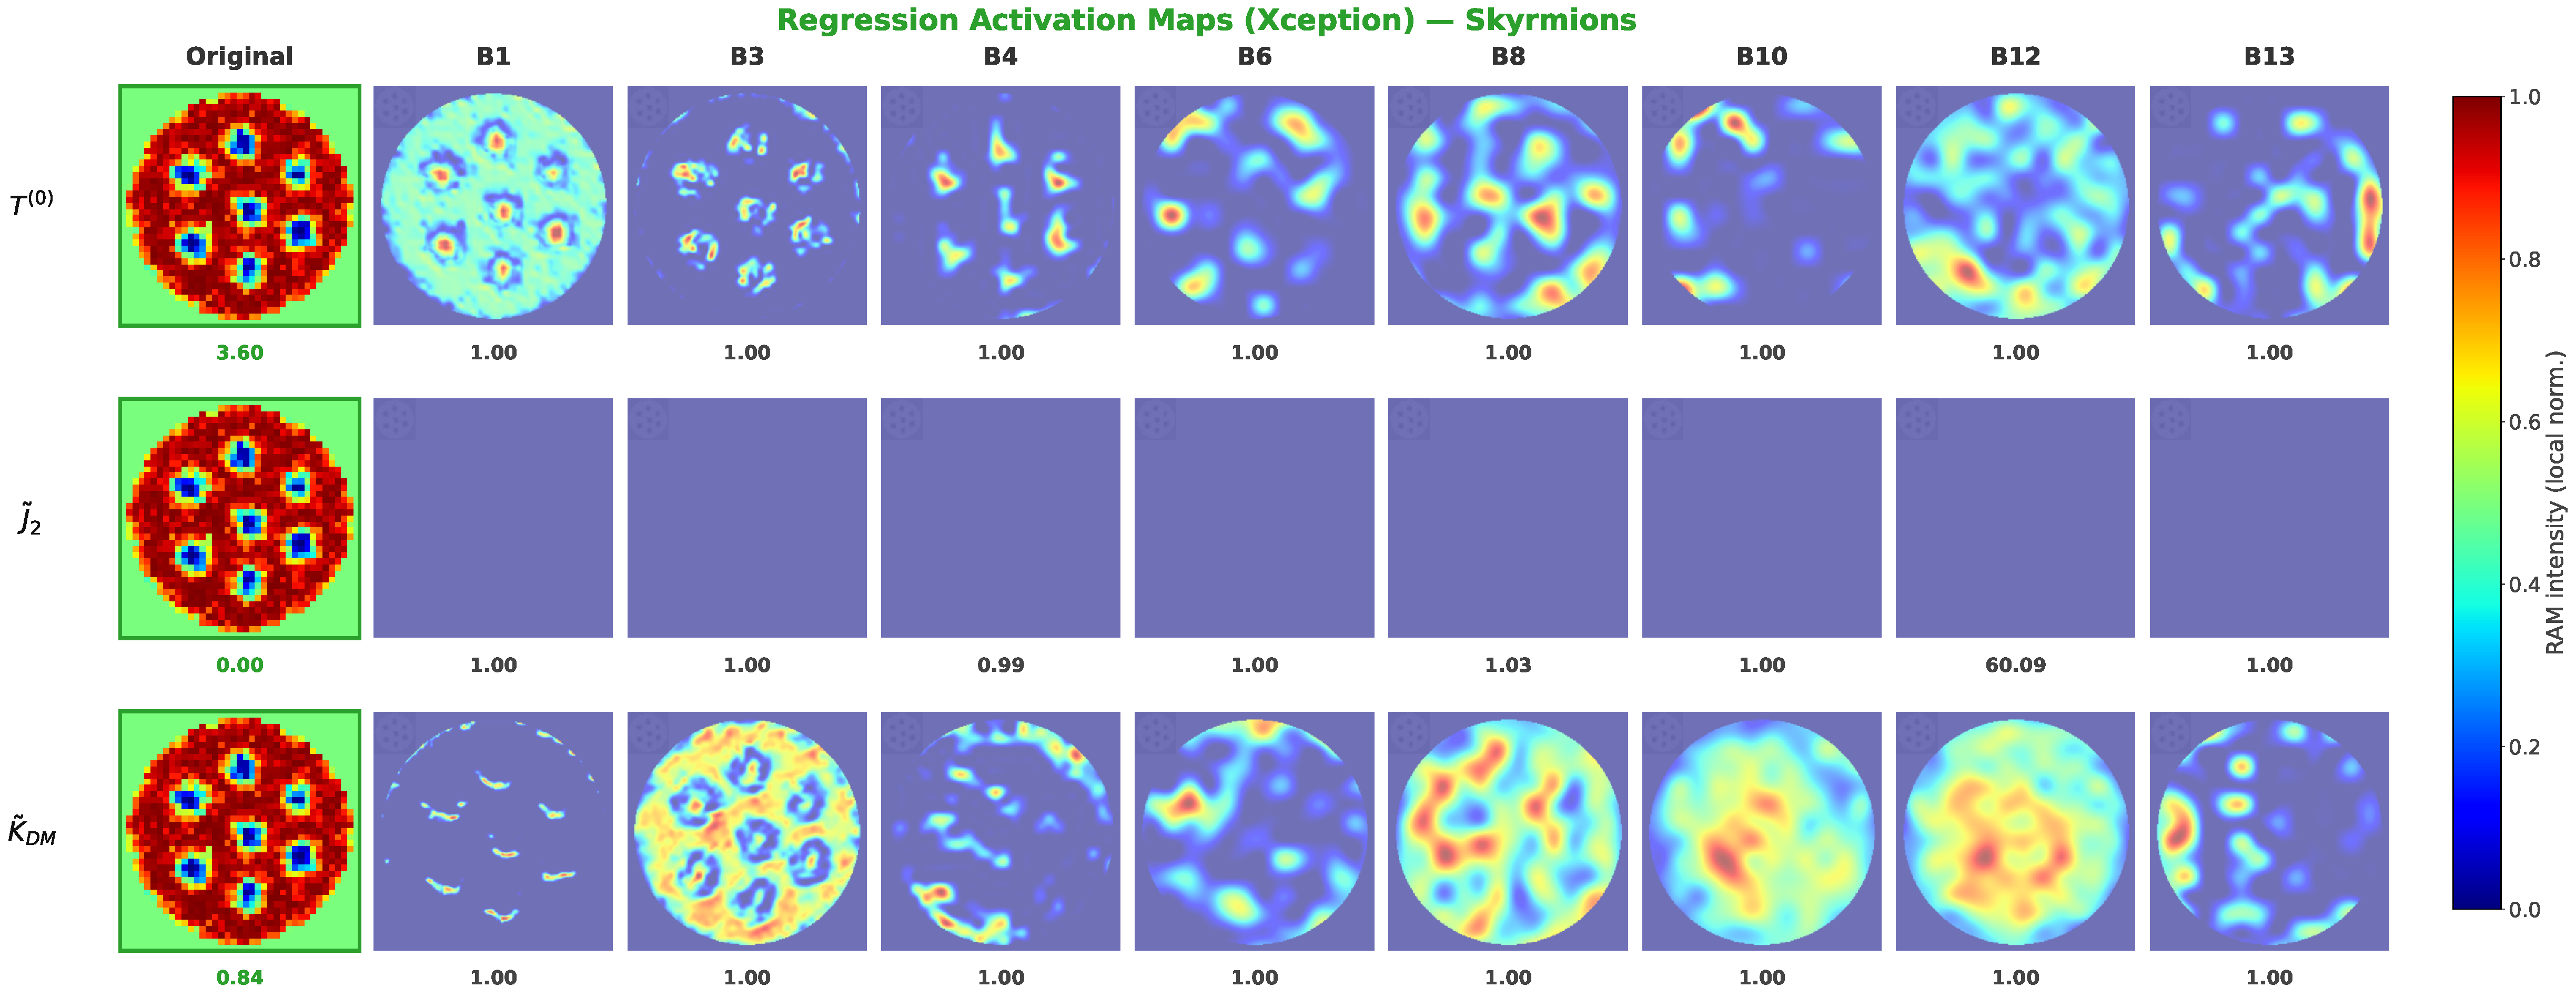
\includegraphics[width=\linewidth, trim=0 0 0 45.5bp, clip]{rams_xception_overlay_Skyrmiones}
    \caption{RAMs $\tilde{\mathcal{R}}_{\text{RAM}}^{(l,p)}$ for the
    Xception architecture in the skyrmion phase. Rows are three
    Hamiltonian parameters $\{T^{(0)}, \tilde{J}_2, \tilde{K}_{DM}\}$;
    columns are network layers from \texttt{block1} (entry,
    $112\times112$) to \texttt{block13} (exit, $14\times14$), with the
    original $s_z$ image in the leftmost column. Each panel overlays
    the RAM (jet colormap) on the magnetization, locally normalized
    per layer. The score below each cell is the fraction of activation
    within the nanodot disk; the value below each original image is
    the ground-truth parameter.}
    \label{fig:rams_xception_unified}
\end{figure*}

To quantify the relative importance of each network layer
and each Hamiltonian parameter in driving the gradient
response, Figure~\ref{fig:rams_xception_bars} presents
the mean maximum RAM activation per layer and variable,
averaged over $N=300$ randomly sampled test images per
magnetic phase. To enable meaningful cross-layer and
cross-parameter comparisons, the raw activation values
were standardized via a global z-score transform across
all layers and variables within each phase, and subsequently
mapped through a sigmoid function
$\sigma\!\left(\frac{x - \mu}{\sigma_x}\right) \in (0,1)$,
where $\mu$ and $\sigma_x$ denote the global mean and
standard deviation of the raw activations for each variable.
This normalization preserves the relative ordering of
activation magnitudes while compressing outliers and
centering the scale around $\sigma = 0.5$, such that
values above this threshold indicate above-average gradient
response for that parameter at that layer depth.

This statistical analysis confirms and extends the
qualitative observations from the spatial maps. Across
all five phases, the sigmoid-normalized activation profile
exhibits a non-monotonic behavior across depth, with a
consistently dominant peak at the terminal exit-flow layer
\texttt{block13\_sepconv2}, where the network aggregates the
high-level semantic representations of the identifiable
parameters ($T^{(0)}$, $\tilde{J}_2$, $\tilde{K}_{DM}$,
$\tilde{K}_{an1}$, and $\tilde{H}_{ex}$). Secondary peaks in
the middle-flow layers (\texttt{block6}--\texttt{block8})
reflect the intermediate stage at which the localized chiral
and domain-wall features are assembled, and are most
pronounced in the ordered skyrmion and Ising phases whose
sharp textures provide the strongest spatial signal. By
contrast, the higher-order exchange constants $\tilde{J}_3$
and $\tilde{J}_4$ exhibit the lowest and least structured
sigmoid activations across all layers and phases,
corroborating their fundamental unidentifiability established
in Section~\ref{sec:dl_results} and confirming that the
Xception backbone has not learned spatially distinctive
features for these parameters --- a direct consequence of
their energetic subordination to the dominant first- and
second-shell exchange. The identifiable anisotropy and field
parameters, in turn, attain their strongest activations in
the phases where they leave a measurable imprint (the
high-anisotropy Ising regime and the out-of-plane-field
configurations), consistent with their successful recovery
in the regression analysis.

\begin{figure*}[!t]
    \centering
    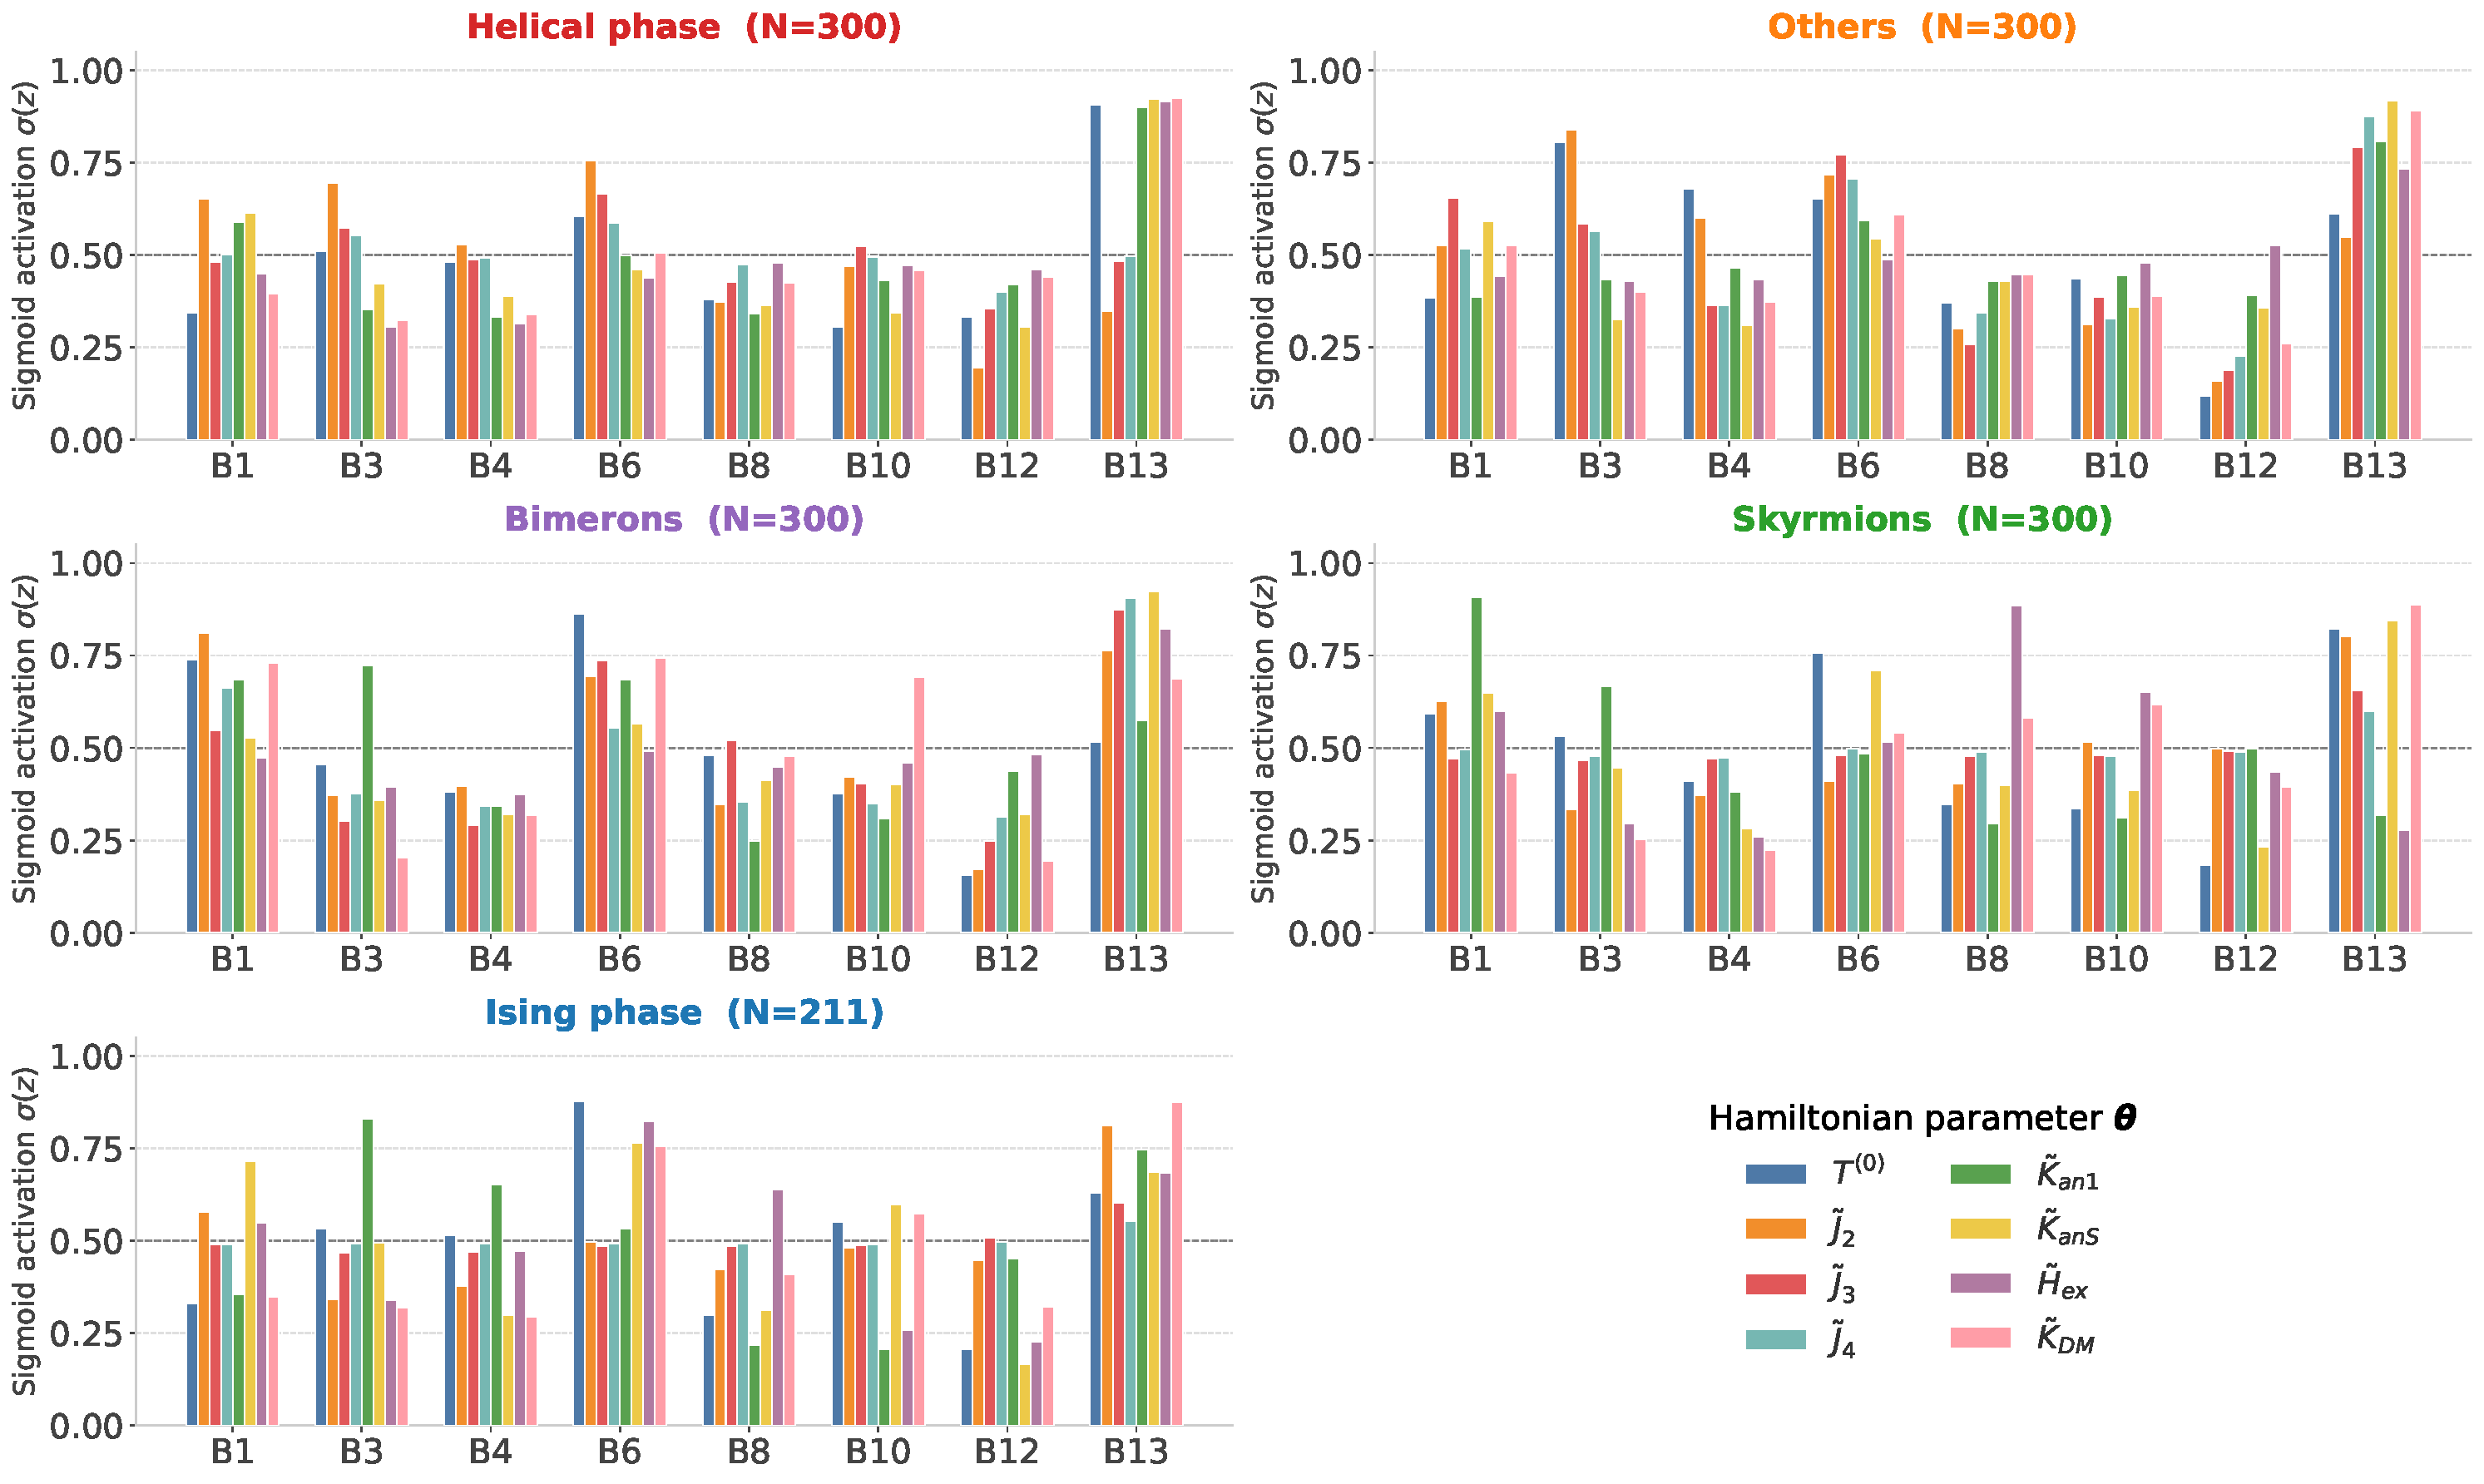
\includegraphics[width=\linewidth]
    {rams_xception_magnitude_bars-2}
    \caption{Mean maximum RAM activation per network layer and
    Hamiltonian parameter $\boldsymbol{\theta}$, averaged over
    $N=300$ test samples per phase ($N=211$ for Ising; Xception CNN),
    measured within the nanodot disk (masked RAM). Activations use a
    per-variable sigmoid normalization
    $\sigma\!\left(\frac{x-\mu}{\sigma_x}\right)$, where values above
    $\sigma=0.5$ indicate above-average response; colors follow the
    parameter nomenclature of Table~\ref{tab:param_ranges}. The
    higher-order exchange constants $\tilde{J}_3$ and $\tilde{J}_4$
    show the lowest activation across all layers and phases,
    confirming their fundamental identifiability limit.}
    \label{fig:rams_xception_bars}
\end{figure*}

%
The RAM analysis thus isolates a physically coherent set of features as the primary drivers of accurate regression: chiral domain-wall boundaries, stripe periodicity, and skyrmion cores. Conversely, the higher-order exchange constants $\tilde{J}_3$ and $\tilde{J}_4$ never acquire spatially concentrated activations, confirming that their limited identifiability is not a consequence of insufficient model capacity but of the fundamental physical constraints of the inverse problem---their energetic subordination to the dominant first- and second-shell exchange, which leaves no distinguishable imprint on the $s_z$ projection. For completeness, the RAM formulation was also derived for the Vision Transformer (Section~\ref{sec:ViT_RAMs}); since Xception is the best-performing model and provides the clearest spatial attributions, the remainder of the interpretability analysis focuses on it.


\subsection{Interpretability Benchmark: RAMs versus Perturbation-Based Attribution}
\label{sec:interpretability_benchmark}

Having established that RAMs isolate physically meaningful spatial features, we now benchmark them quantitatively against the perturbation-based attribution baselines introduced in Section~\ref{sec:xai_baselines}---LIME, SHAP, and SF-SHAP---using the deletion protocol of Equations~\ref{eq:deletion_dev}--\ref{eq:deletion_auc}. The comparison targets both fidelity (how faithfully each map localizes the pixels that drive the prediction) and computational cost.

The perturbation baselines operate on superpixels rather than individual pixels, so the spatial granularity of the segmentation directly conditions their behavior. To fix this granularity on a physical basis, the number of SLIC segments was chosen so that the resulting superpixel equivalent diameter matches the characteristic magnetic domain width of the dataset ($\approx 4.9$~px). As shown in Figure~\ref{fig:slic_criterion}, this criterion is satisfied at $N = 100$ segments, which we adopt for all perturbation baselines, ensuring that each interpretable region corresponds to one coherent magnetic domain rather than to an arbitrary pixel cluster.

\begin{figure}[htbp]
    \centering
    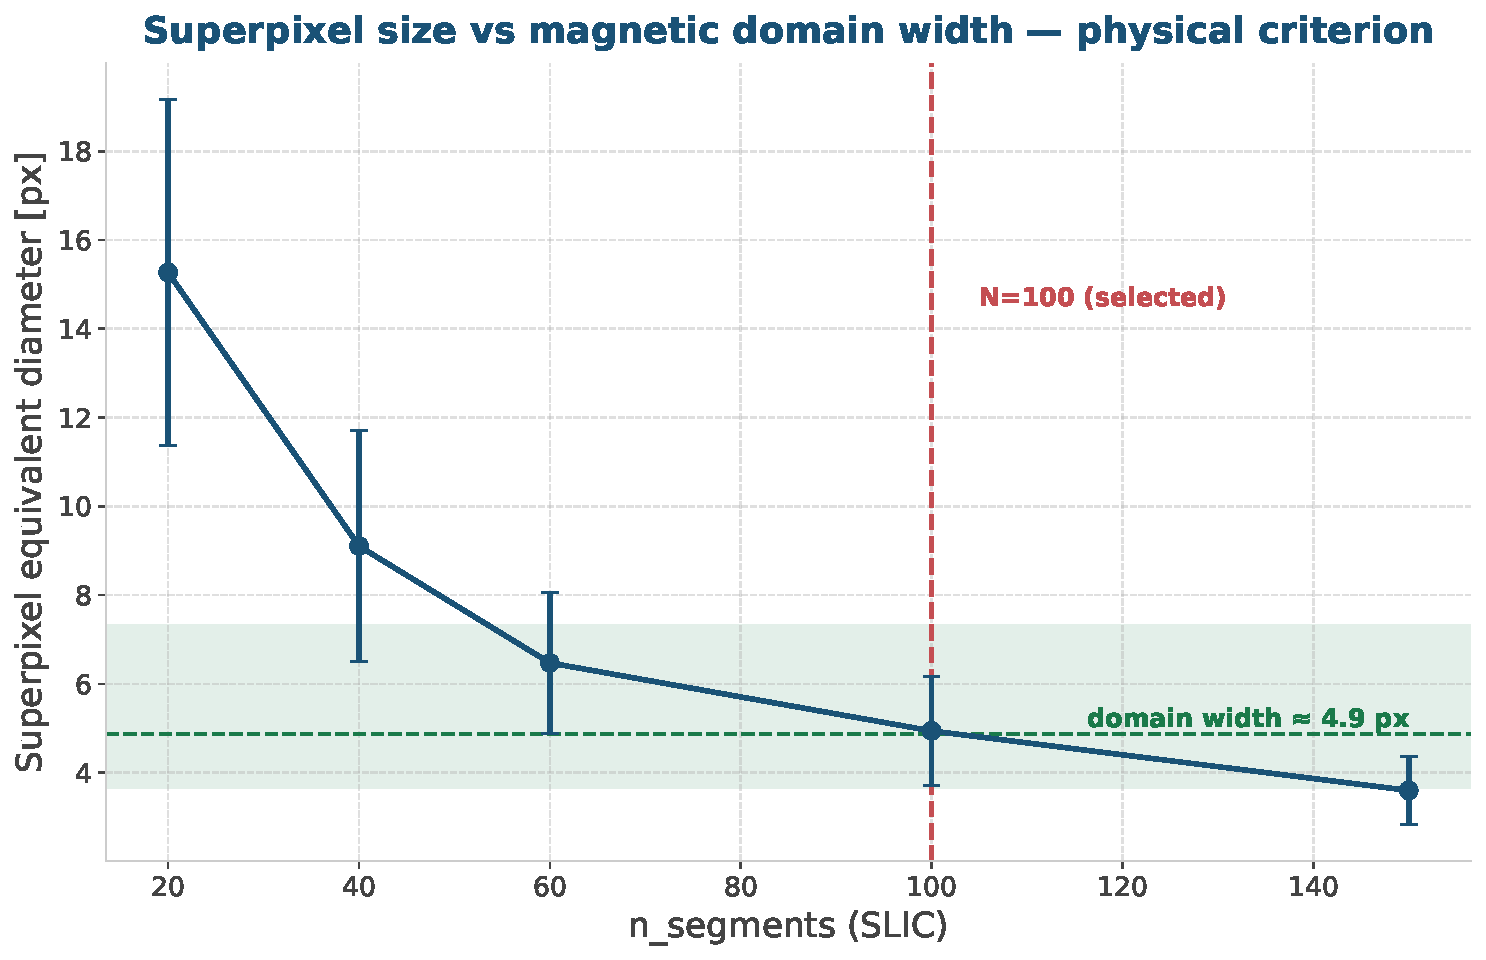
\includegraphics[width=\linewidth, trim=0 0 0 36.9bp, clip]{slic_physical_criterion}
    \caption{Physical criterion for the SLIC segmentation used by the perturbation-based baselines. The superpixel equivalent diameter is plotted against the number of SLIC segments; the selected value $N=100$ (dashed red) yields superpixels whose size matches the characteristic magnetic domain width ($\approx 4.9$~px, dashed green), so that each interpretable region corresponds to a single magnetic domain.}
    \label{fig:slic_criterion}
\end{figure}

Figure~\ref{fig:deletion_comparison} reports the deletion curves for the three most representative parameters, and Figure~\ref{fig:deletion_auc} resolves the corresponding deletion AUC per magnetic phase. Two physically consistent trends emerge. First, for the spatially localized parameters---most notably the DMI strength $\tilde{K}_{DM}$---all attribution methods, including RAMs, degrade the prediction far more rapidly than the random-relevance baseline, and they do so most strongly in the ordered skyrmion and Ising phases where the chiral features are sharpest. This confirms that RAMs genuinely localize the pixels that carry the DMI signal, with a deletion AUC of the same order as the perturbation methods. Second, for the global thermodynamic parameter $T^{(0)}$ the situation is qualitatively reversed: no attribution method separates from---and the random baseline in fact matches or exceeds---the localized methods. This behavior is physically expected rather than a shortcoming of the attributions: the annealing temperature is not associated with any specific sector of the magnetic domain but is an \emph{ambient} property encoded in the overall degree of order of the texture. Consequently, general (random) deletions distributed across the whole nanodot perturb the global order more effectively than deletions concentrated on a few ``most relevant'' regions, so that attempting to localize $T^{(0)}$ offers no advantage over uniform removal. The deletion metric thus correctly reflects that $T^{(0)}$ is a delocalized, environment-like parameter, in contrast to the spatially bound signatures of $\tilde{J}_2$ and $\tilde{K}_{DM}$.

\begin{figure*}[!t]
    \centering
    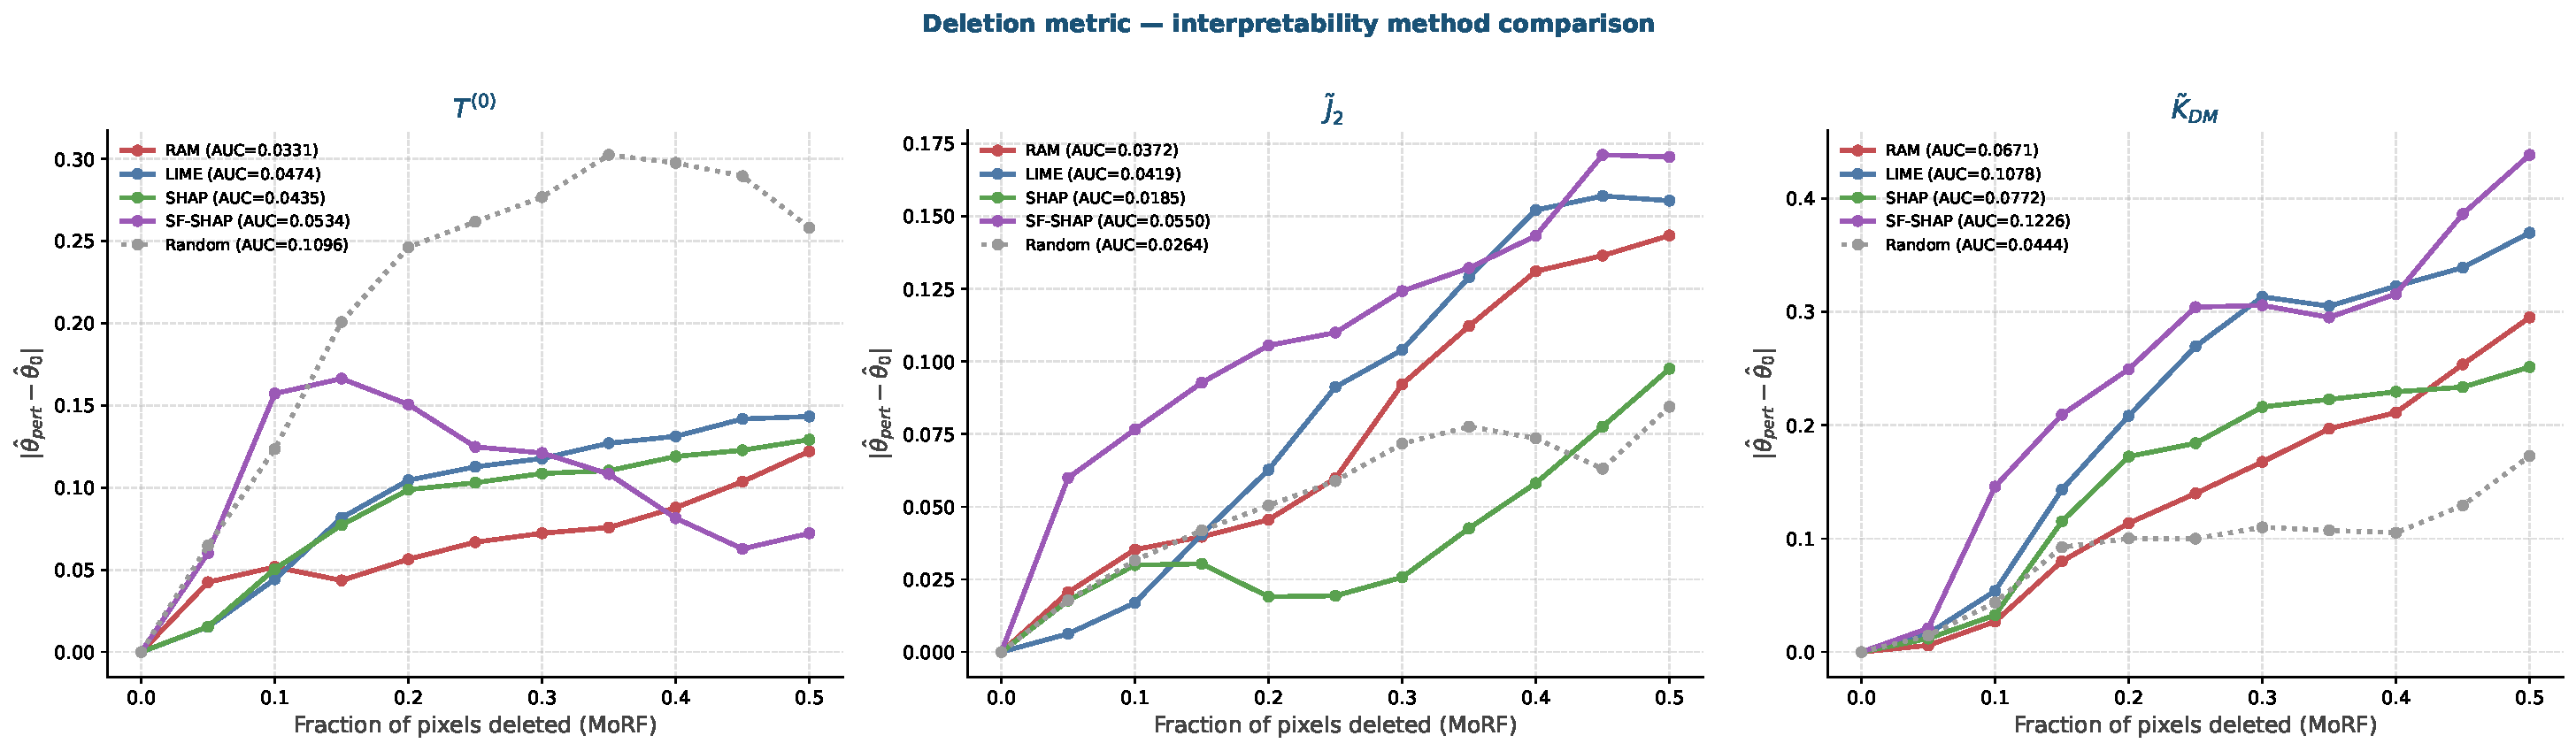
\includegraphics[width=\linewidth, trim=0 0 0 32.6bp, clip]{deletion_comparison}
    \caption{Deletion curves (Most Relevant First) for RAM, LIME, SHAP, and SF-SHAP, with a random-relevance lower bound, for the three representative parameters $T^{(0)}$, $\tilde{J}_2$, and $\tilde{K}_{DM}$. The vertical axis is the induced deviation $|\hat{\theta}_{\text{pert}}-\hat{\theta}_0|$ as the most relevant pixels are progressively replaced by the baseline; the area under each curve (AUC, in the legend) quantifies faithfulness.}
    \label{fig:deletion_comparison}
\end{figure*}

\begin{figure*}[!t]
    \centering
    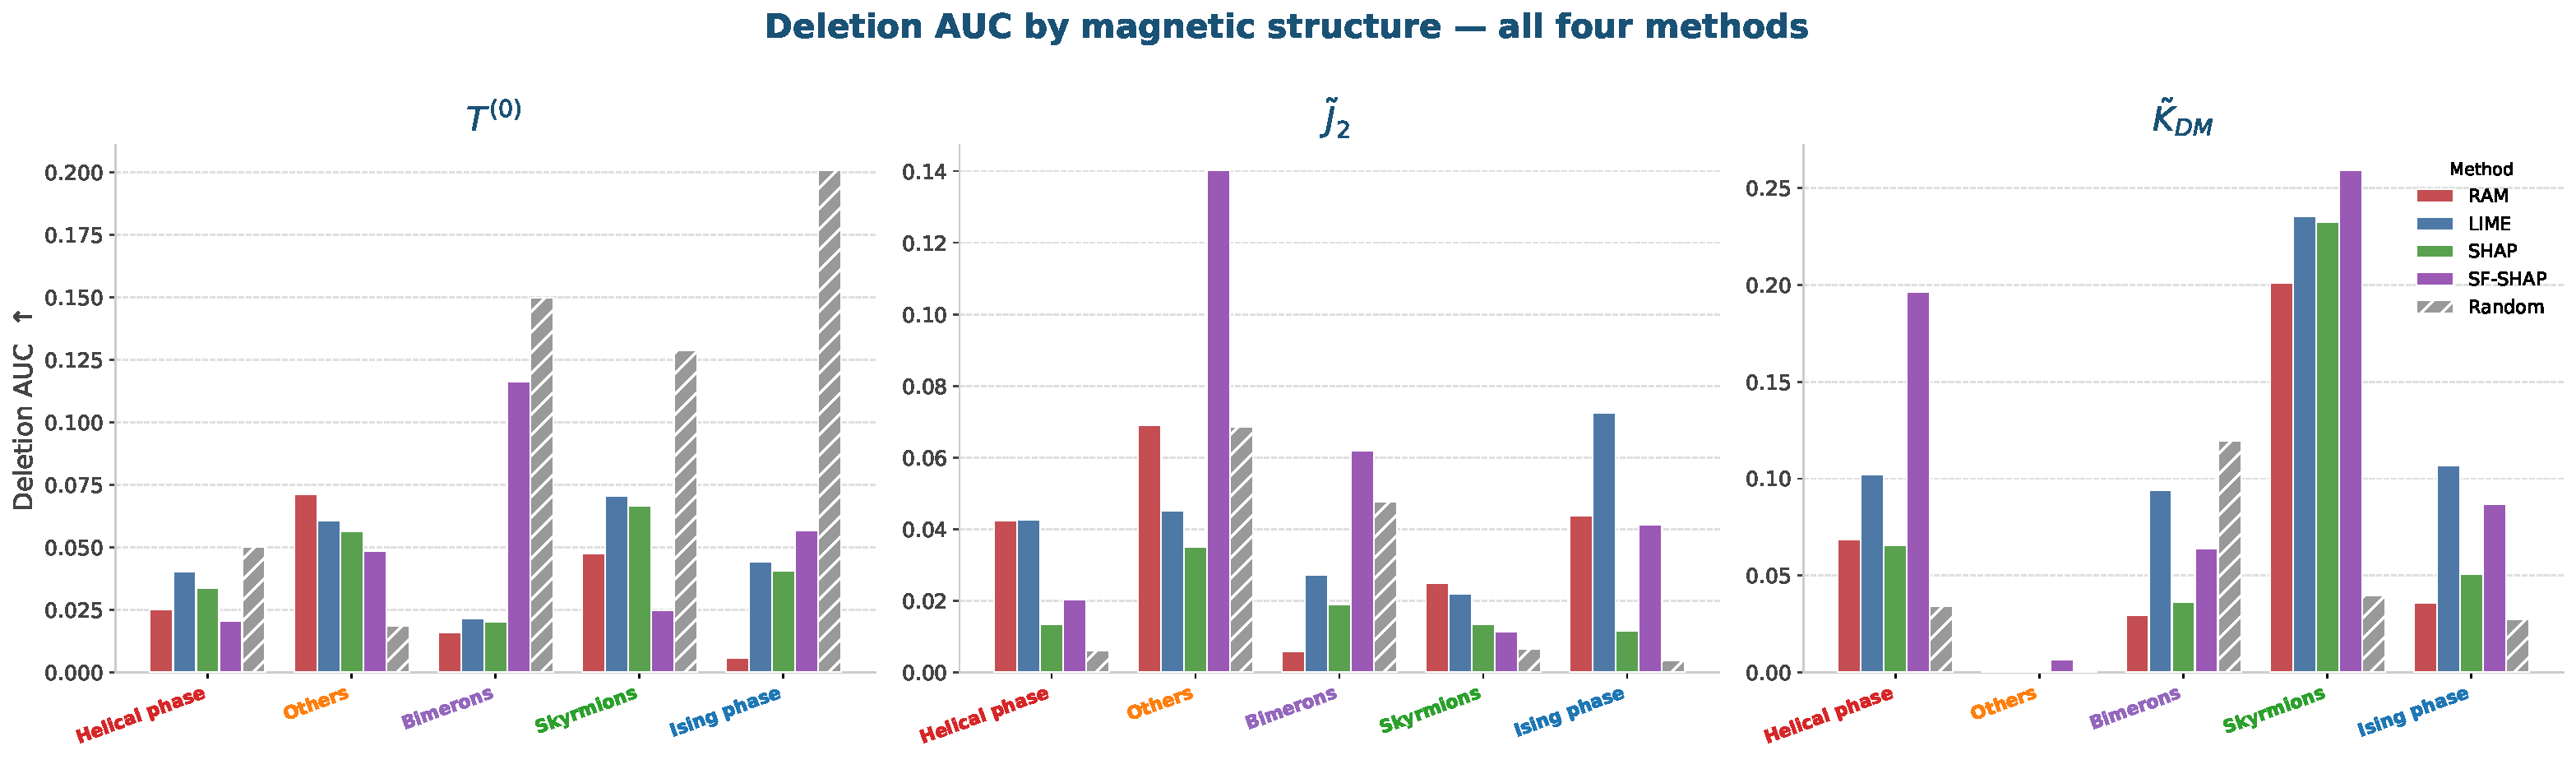
\includegraphics[width=\linewidth, trim=0 0 0 35.5bp, clip]{deletion_auc_by_structure}
    \caption{Deletion AUC resolved by magnetic phase for RAM, LIME, SHAP, and SF-SHAP (with the random baseline), for $T^{(0)}$, $\tilde{J}_2$, and $\tilde{K}_{DM}$; a higher AUC indicates a more faithful attribution.}
    \label{fig:deletion_auc}
\end{figure*}

The decisive advantage of RAMs lies in their computational cost. Figure~\ref{fig:interp_cost} contrasts the cost of producing a single relevance map. Being gradient-based, a RAM requires exactly one backward pass---i.e., a single model evaluation---whereas the perturbation baselines must query the model over many masked coalitions: of order $10^3$ evaluations for LIME and SHAP and $2^{7}=128$ for SF-SHAP. This translates into a measured wall-clock cost per map that is one to two orders of magnitude lower for RAMs than for any perturbation method. RAMs therefore deliver a faithfulness competitive with established attribution techniques while remaining tractable for the high-throughput, per-sample interpretability that materials-characterization pipelines require---an efficiency that the perturbation-based methods, by construction, cannot match.

\begin{figure}[htbp]
    \centering
    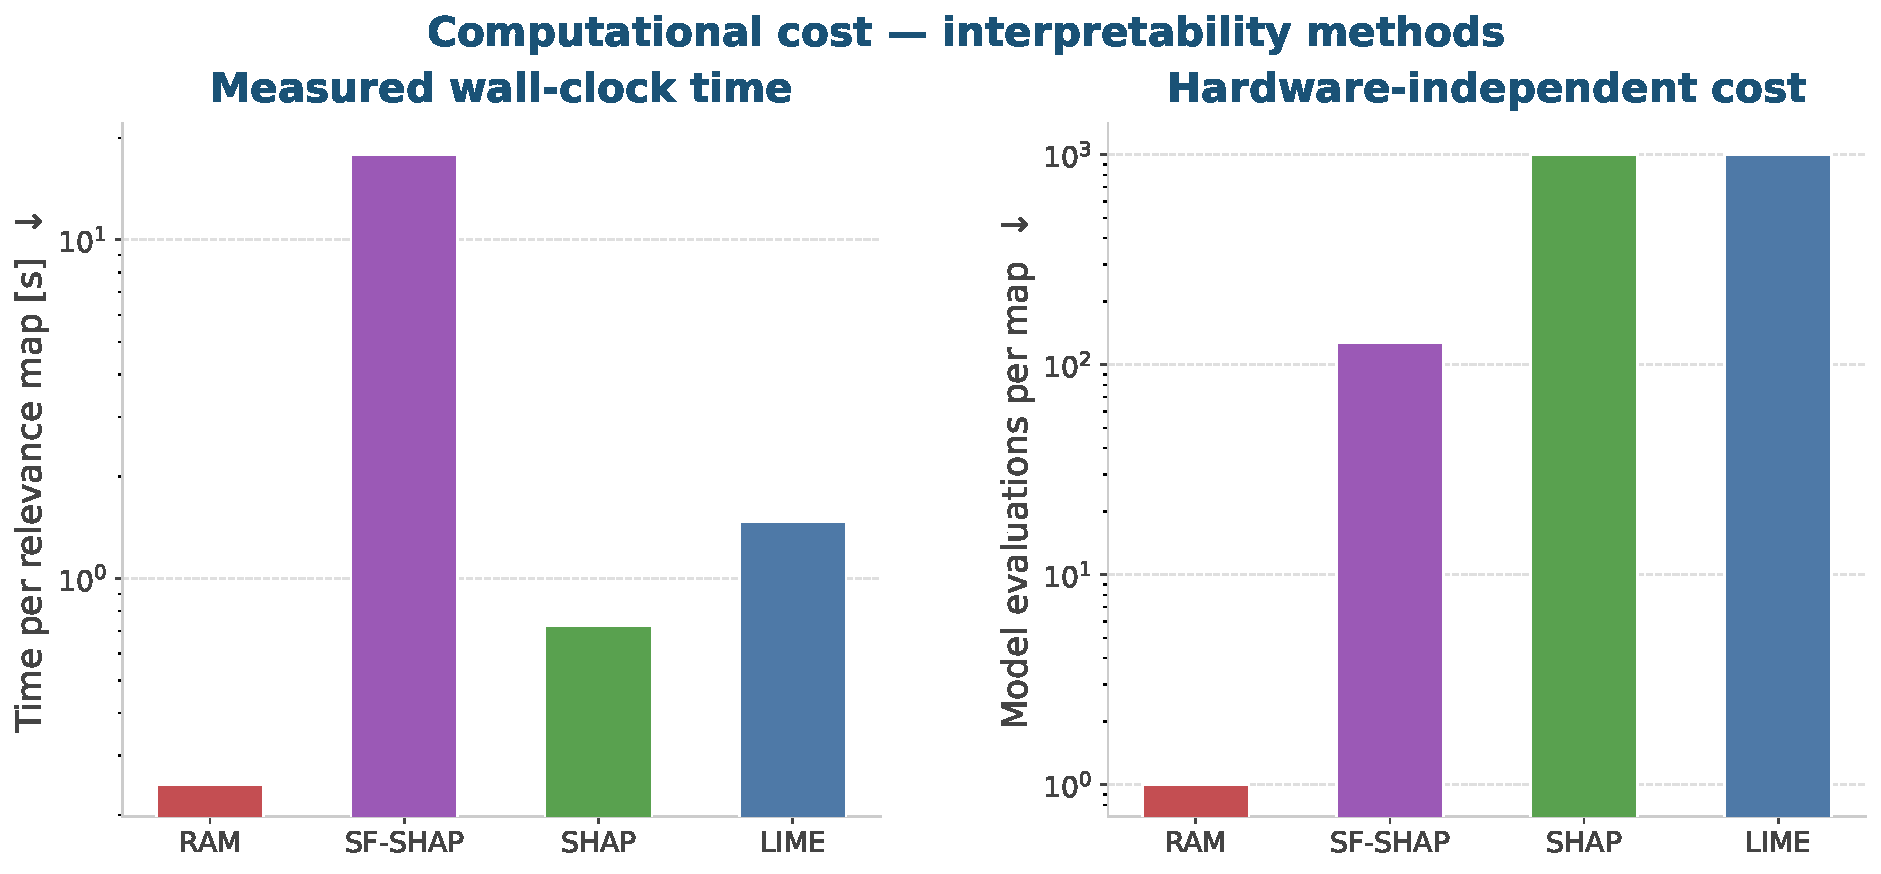
\includegraphics[width=\linewidth, trim=0 0 0 29.4bp, clip]{interpretability_cost}
    \caption{Computational cost of the interpretability methods. Left: measured wall-clock time per relevance map (log scale). Right: number of model evaluations per map (log scale). A RAM requires a single backward pass, against $\sim\!10^3$ evaluations for LIME and SHAP and $128$ for SF-SHAP.}
    \label{fig:interp_cost}
\end{figure}


\subsection{Limitations}
\label{sec:limitations}

Despite the promising results demonstrated across the 
regression, clustering, and interpretability analyses, 
the proposed framework presents several inherent 
limitations that must be explicitly acknowledged to 
contextualize its applicability and guide future 
research directions.

The most fundamental limitation of the framework is the intrinsic
partial observability of the extended Heisenberg Hamiltonian from
two-dimensional magnetization images. As established in
Section~\ref{sec:dl_results} and confirmed by the
RAM-based interpretability analysis of
Section~\ref{sec:rams_results}, the projection of the
three-dimensional spin configuration onto the out-of-plane component
$s_z$ of the central layer of the nanodot constitutes a
dimensionality reduction that irreversibly discards physical
information. While the dataset enrichment adopted in this work---the
out-of-plane field configurations and the extended anisotropy
range---renders six of the eight parameters recoverable, the
higher-order exchange constants $\tilde{J}_3$ and $\tilde{J}_4$ remain
fundamentally unidentifiable: their energetic contribution is
subordinated to the dominant first- and second-shell exchange, so
they leave no distinguishable signature in the $s_z$ texture,
regardless of model capacity or architecture. A related, milder
limitation affects the surface anisotropy $\tilde{K}_{anS}$, which is
recovered only partially because the input images are extracted
exclusively from the central discrete layer
($z = \lfloor \breve{L}/2 \rfloor$) of the three-dimensional nanodot
lattice, discarding the depth-resolved spin structure that encodes
the surface-to-bulk anisotropy ratio
$\tilde{K}_{anS}/\tilde{K}_{an1}$. Recovering these remaining
parameters with high fidelity would require either access to the full
three-dimensional spin vector field $\mathbf{S}_i = (s_x, s_y, s_z)$
at each lattice site, or volumetric magnetization inputs obtained
through multi-layer or tomographic magnetic imaging techniques. This
is not a limitation of the deep learning models themselves but of
the observational modality assumed by the framework, which mimics
the two-dimensional projection inherent to most experimental
magnetic imaging techniques such as magnetic force microscopy or
Lorentz transmission electron microscopy.

The dataset utilized in this study consists entirely 
of simulated magnetization images generated through 
the atomistic Monte Carlo framework described in 
Section~\ref{sec:montecarlo_sim}. While the 
simulation protocol incorporates physically realistic 
finite-size effects, cylindrical boundary conditions, 
and thermodynamic relaxation via simulated annealing, 
it does not account for several experimental 
phenomena that are routinely present in real magnetic 
nanodot imaging. These include thermal noise and 
instrument-specific point spread functions inherent 
to the imaging apparatus, crystallographic defects, 
vacancies, and grain boundaries that break the 
assumed periodic lattice symmetry, surface 
reconstruction effects that modify the effective 
exchange and DMI parameters at the physical boundary 
of the nanodot, and substrate-induced strain fields 
that can renormalize the bulk Hamiltonian parameters. 
As a consequence, a model trained exclusively on 
simulated data may exhibit significant performance 
degradation when applied to experimentally acquired 
magnetization images --- a domain shift problem 
that has not been quantified in the present work. 
Bridging this simulation-to-experiment gap would 
require either transfer learning with a small set 
of experimentally labeled samples or the 
incorporation of physics-informed data augmentation 
strategies that realistically replicate experimental
noise sources.

A further limitation concerns the internal structure of the sampled parameter space. The dataset spans two mechanisms for stabilizing modulated textures---exchange frustration (driven by $\tilde{J}_2$) and the chiral DMI (driven by $\tilde{K}_{DM}$)---which were deliberately activated in a mutually exclusive fashion to isolate and compare their individual contributions, and were subsequently unified into a single training corpus. While this design cleanly separates the two mechanisms and demonstrates that both can independently generate analogous modulated states, it does not include configurations in which the two interactions coexist and compete simultaneously, as may occur in real materials. Extending the dataset to jointly sample $\tilde{J}_2$ and $\tilde{K}_{DM}$ would allow the model to learn their combined effect and is a natural direction for future work.

From a deep learning perspective, the RAM-based
interpretability framework introduced in this work 
provides spatially resolved gradient attributions 
that are physically consistent and architecturally 
agnostic. However, RAMs share the fundamental 
limitations of all gradient-based saliency methods: 
the attribution maps reflect the local sensitivity 
of the objective function $\mathcal{O}_p$ to spatial 
activations at the point of evaluation, but do not 
provide a globally faithful explanation of the 
model's decision function across the full parameter 
space. In particular, gradient saturation in deeply 
nonlinear networks can produce spatially diffuse 
or spurious attributions for parameters with low 
predictive signal --- precisely the degenerate 
parameters identified in this study. Furthermore, 
the current RAM formulation computes a single 
attribution map per image per parameter, which 
does not capture the stochastic uncertainty in 
the attribution due to the non-deterministic 
elements of the forward pass. Future extensions 
could incorporate ensemble-based or Bayesian 
attribution methods to provide confidence intervals 
on the spatial interpretability maps, which would 
be particularly valuable for the physically 
ambiguous parameter--phase combinations identified 
in Section~\ref{sec:rams_results}.

A more fundamental limitation is intrinsic to the observable
itself: because the framework operates on the out-of-plane
$s_z$ projection, parameters whose signature lies in the
in-plane components---or whose energetic contribution is
subordinated to the dominant exchange, as for
$\tilde{J}_3$ and $\tilde{J}_4$---cannot be recovered, a
boundary that would require chirality-sensitive or fully
three-dimensional observables to overcome.

\section{Conclusions}
\label{sec:conclusions}

This work introduced a regression-based explainable deep learning
framework for the inverse estimation of Hamiltonian parameters from
two-dimensional magnetization images of magnetic nanodots. The
proposed methodology integrates atomistic Monte Carlo simulations
under a physically rigorous extended Heisenberg Hamiltonian with eight
free parameters, five state-of-the-art deep learning architectures, an
unsupervised latent space analysis via UMAP and density-based
clustering, and a novel spatial interpretability formulation RAMs that generalizes gradient-based
activation mapping to the continuous regression domain for both
convolutional and transformer-based architectures.
 
Among the five evaluated architectures, Xception achieved the highest
overall regression accuracy, although all models---including the
compact conventional CNN baseline trained from scratch---performed
comparably, demonstrating that estimation accuracy is governed by the
physical information available in the $s_z$ projection rather than by
model capacity or pretraining. Six of the eight Hamiltonian parameters
were recovered with high fidelity: the annealing temperature $T^{(0)}$,
the second-shell exchange $\tilde{J}_2$, the DMI strength
$\tilde{K}_{DM}$, the bulk anisotropy $\tilde{K}_{an1}$, and the
external Zeeman field $\tilde{H}_{ex}$, with the surface anisotropy
$\tilde{K}_{anS}$ at an intermediate level. This broad identifiability
was made possible by the deliberate enrichment of the dataset with
out-of-plane field configurations---coupling the Zeeman term to the
observable $s_z$ component---and an extended anisotropy range. By
contrast, the higher-order exchange constants $\tilde{J}_3$ and
$\tilde{J}_4$ exhibited near-zero $R^2$ across all architectures,
establishing that the fundamental limitation of the inverse problem is
not architectural capacity but the intrinsic partial observability of
these subordinate interactions from the two-dimensional projection.

Beyond the aggregate regression performance, the UMAP projection of the
Xception latent representations revealed that the model autonomously
organized the magnetization textures into geometrically distinct and
physically interpretable regions of the embedding space, without any
explicit supervision of magnetic phase labels. Density-based clustering
identified five dominant magnetic phase categories---helical, skyrmion,
Ising, bimeron, and a heterogeneous \textit{others} group. The
per-phase regression analysis confirmed that the model achieves its
highest accuracy within the most ordered phases (skyrmion and Ising,
$R^2 \gtrsim 0.94$ across the identifiable parameters), where the
magnetization texture carries the most discriminative physical
information, while the disordered and mixed-chirality configurations
concentrate the largest errors.

The proposed RAMs formulation successfully extended gradient-based
activation mapping to the continuous regression setting through a
scale-invariant Gaussian error-decay objective
$\mathcal{O}_p = \exp(-\gamma_p(\theta_p - \hat{\theta}_p)^2)$,
providing physically interpretable spatial attribution maps for each
Hamiltonian parameter independently. For the Xception architecture, the
layer-resolved RAM analysis revealed a physically consistent
hierarchical decoupling across network depth: early entry-flow layers
capture fine-grained domain periodicity and chiral winding at high
spatial resolution, while deeper middle-flow and exit-flow layers
consolidate these local features into coarser, topologically meaningful
representations, with the DMI attributions localizing on the skyrmion
cores that encode it. Benchmarked against the LIME, SHAP, and exact
spatial-frequency Shapley baselines through a deletion protocol, RAMs
attained a competitive spatial faithfulness---far above the random
baseline for the localized parameters---while requiring a single
backward pass per map, one to two orders of magnitude cheaper than the
perturbation-based methods. This combination of physical faithfulness
and computational efficiency makes RAMs practical for per-sample
interpretability in high-throughput materials characterization.
 
Taken together, the results of this study demonstrate that
regression-based deep learning, combined with physically motivated
interpretability methods, constitutes a viable and physically
meaningful approach to the inverse Hamiltonian estimation problem in
magnetic nanostructures. The proposed RAMs framework is
architecture-agnostic and directly applicable to any continuous
regression task where spatial attribution of physical parameters is
required, extending beyond magnetic nanodots to other physical systems
characterized by spatially resolved imaging modalities.
 
Several directions merit investigation in future work. First,
incorporating the full three-dimensional spin vector field
$\mathbf{S}_i = (s_x, s_y, s_z)$ or multi-layer volumetric
magnetization images as input would substantially reduce the partial
observability constraint and improve the identifiability of the
parameters that remain elusive under the $s_z$-only observation---the
surface anisotropy $\tilde{K}_{anS}$ and, in particular, the
higher-order exchange constants $\tilde{J}_3$ and $\tilde{J}_4$. Second, domain adaptation strategies, including physics-informed data augmentation and few-shot transfer
learning from experimentally labeled samples, are necessary to
bridge the simulation-to-experiment gap and enable direct application
to real magnetic imaging data. Third, extending the RAM formulation to
incorporate uncertainty quantification through ensemble-based or
Bayesian attribution methods would provide confidence intervals on the
spatial interpretability maps, which are particularly valuable for
physically ambiguous parameter--phase combinations near topological
phase boundaries. Finally, the integration of the proposed framework
with active learning strategies, where the model identifies the
most informative parameter combinations to simulate next, could
dramatically accelerate the construction of training datasets for
high-dimensional Hamiltonian spaces, enabling the extension of the
inverse estimation approach to more complex magnetic systems with
larger numbers of competing energetic contributions.


\section*{Acknowledgments}
Under grants provided by the research project: "Aprendizaje automático aplicado a la predicción eficiente de propiedades magnéticas de nanopartículas como soporte a la generación de dispositivos electrónicos" Hermes 62642, funded by Universidad Nacional de Colombia. Also, A. Alvarez thanks to the project: "Estimación de la capacidad de generación de energía eléctrica del agua coproducida en campos de petróleo y gas en Colombia a partir de técnicas de aprendizaje automático informado por la física," Code 111908, funded by 951-2024 Convocatoria fortalecimiento del conocimiento científico y tecnológico de las fuentes - Minciencias.ñkm

\section*{Declaration of generative AI and AI-assisted technologies in the manuscript preparation process}

During the preparation of this work the author(s) used Gemini and Claude in order to enhance the writing style. After using this tool/service, the author(s) reviewed and edited the content as needed and take(s) full responsibility for the content of the published article.



%% Loading bibliography style file
%\bibliographystyle{model1-num-names}
%\bibliographystyle{cas-model2-names}
\bibliographystyle{ieeetr}

% Loading bibliography database
\begin{thebibliography}{10}

\bibitem{heinrich2021quantum}
A.~J. Heinrich, W.~D. Oliver, L.~M. Vandersypen, A.~Ardavan, R.~Sessoli, D.~Loss, A.~B. Jayich, J.~Fernandez-Rossier, A.~Laucht, and A.~Morello, ``Quantum-coherent nanoscience,'' {\em Nat. Nanotechnol.}, vol.~16, no.~12, pp.~1318--1329, 2021.

\bibitem{fert2024electrical}
A.~Fert, R.~Ramesh, V.~Garcia, F.~Casanova, and M.~Bibes, ``Electrical control of magnetism by electric field and current-induced torques,'' {\em Rev. Mod. Phys.}, vol.~96, no.~1, p.~015005, 2024.

\bibitem{issa2013magnetic}
B.~Issa, I.~M. Obaidat, B.~A. Albiss, and Y.~Haik, ``Magnetic nanoparticles: surface effects and properties related to biomedicine applications,'' {\em Int. J. Mol. Sci.}, vol.~14, no.~11, pp.~21266--21305, 2013.

\bibitem{charalampidis2023metadynamics}
I.~Charalampidis and J.~Barker, ``Metadynamics calculations of the effect of thermal spin fluctuations on skyrmion stability,'' {\em arXiv preprint arXiv:2310.03169}, 2023.

\bibitem{yu2021magnetic}
X.~Yu, ``Magnetic imaging of various topological spin textures and their dynamics,'' {\em J. Magn. Magn. Mater.}, vol.~539, p.~168332, 2021.

\bibitem{tokura2020magnetic}
Y.~Tokura and N.~Kanazawa, ``Magnetic skyrmion materials,'' {\em Chem. Rev.}, vol.~121, no.~5, pp.~2857--2897, 2020.

\bibitem{rohart2013skyrmion}
S.~Rohart and A.~Thiaville, ``Skyrmion confinement in ultrathin film nanostructures in the presence of dzyaloshinskii-moriya interaction,'' {\em Phys. Rev. B}, vol.~88, no.~18, p.~184422, 2013.

\bibitem{kong2023quantifying}
J.~F. Kong, Y.~Ren, M.~N. Tey, P.~Ho, K.~H. Khoo, X.~Chen, and A.~Soumyanarayanan, ``Quantifying the magnetic interactions governing chiral spin textures using deep neural networks,'' {\em ACS Appl. Mater. Interfaces}, vol.~16, no.~1, pp.~1025--1032, 2023.

\bibitem{evans2014atomistic}
R.~F. Evans, W.~J. Fan, P.~Chureemart, T.~A. Ostler, M.~O. Ellis, and R.~W. Chantrell, ``Atomistic spin model simulations of magnetic nanomaterials,'' {\em J. Phys.: Condens. Matter}, vol.~26, no.~10, p.~103202, 2014.

\bibitem{aldarawsheh2023intrinsic}
A.~Aldarawsheh, M.~Sallermann, M.~Abusaa, and S.~Lounis, ``Intrinsic n{\'e}el antiferromagnetic multimeronic spin textures in ultrathin films,'' {\em J. Phys. Chem. Lett.}, vol.~14, no.~40, pp.~8970--8978, 2023.

\bibitem{back20202020}
C.~Back, V.~Cros, H.~Ebert, K.~Everschor-Sitte, A.~Fert, M.~Garst, T.~Ma, S.~Mankovsky, T.~Monchesky, M.~Mostovoy, {\em et~al.}, ``The 2020 skyrmionics roadmap,'' {\em J. Phys. D: Appl. Phys.}, vol.~53, no.~36, p.~363001, 2020.

\bibitem{murakami2022inverse}
R.~Murakami, M.~Mizumaki, I.~Akai, and H.~Shouno, ``Inverse estimation of parameters for the magnetic domain via dynamics matching using visual-perceptive similarity,'' {\em Sci. Technol. Adv. Mater.: Methods}, vol.~2, no.~1, pp.~139--152, 2022.

\bibitem{kwon2020magnetic}
H.~Y. Kwon, H.~Yoon, C.~Lee, G.~Chen, K.~Liu, A.~Schmid, Y.~Wu, J.~Choi, and C.~Won, ``Magnetic hamiltonian parameter estimation using deep learning techniques,'' {\em Sci. Adv.}, vol.~6, no.~39, p.~eabb0872, 2020.

\bibitem{nguyen2022cooperative}
T.~N.~H. Nguyen, L.~Rasabathina, O.~Hellwig, A.~Sharma, G.~Salvan, S.~Yochelis, Y.~Paltiel, L.~T. Baczewski, and C.~Tegenkamp, ``Cooperative effect of electron spin polarization in chiral molecules studied with non-spin-polarized scanning tunneling microscopy,'' {\em ACS Appl. Mater. Interfaces}, vol.~14, no.~33, pp.~38013--38020, 2022.

\bibitem{zhao2025overview}
J.~Zhao, L.~Bai, S.~Li, Z.~Cao, Y.~Peng, J.~Bai, X.~Cai, X.~Shi, X.~Lin, G.~Wei, {\em et~al.}, ``An overview of advanced instruments for magnetic characterization and measurements,'' {\em Frontiers in Electronics}, vol.~6, p.~1645594, 2025.

\bibitem{gaida2023lorentz}
J.~H. Gaida, H.~Louren{\c{c}}o-Martins, S.~V. Yalunin, A.~Feist, M.~Sivis, T.~Hohage, F.~J. Garc{\'\i}a~de Abajo, and C.~Ropers, ``Lorentz microscopy of optical fields,'' {\em Nat. Commun.}, vol.~14, no.~1, p.~6545, 2023.

\bibitem{d2023micromagnetic}
M.~d'Aquino, S.~Perna, M.~Pancaldi, R.~Hertel, S.~Bonetti, and C.~Serpico, ``Micromagnetic study of inertial spin waves in ferromagnetic nanodots,'' {\em Phys. Rev. B}, vol.~107, no.~14, p.~144412, 2023.

\bibitem{lepadatu2021micromagnetic}
S.~Lepadatu, ``Micromagnetic monte carlo method with variable magnetization length based on the landau--lifshitz--bloch equation for computation of large-scale thermodynamic equilibrium states,'' {\em J. Appl. Phys.}, vol.~130, no.~16, 2021.

\bibitem{yin2023computational}
X.~Yin, {\em Computational Materials Design: Integrating Physics With Optimization and Machine Learning}.
\newblock PhD thesis, Carnegie Mellon University, 2023.

\bibitem{karnatov2025analysis}
S.~Karnatov, ``Analysis of psnr, ssim, lpips metrics in the context of human perception of visual similarity,'' {\em Transport systems and technologies}, no.~46, 2025.

\bibitem{lee2024deep}
W.~S. Lee, T.~Song, and K.-M. Kim, ``Deep learning methods for hamiltonian parameter estimation and magnetic domain image generation in twisted van der waals magnets,'' {\em Mach. Learn.: Sci. Technol.}, vol.~5, no.~2, p.~025073, 2024.

\bibitem{chen2024data}
Y.~Chen, Q.~Yang, Y.~Li, H.~Zhang, and C.~Zhang, ``Data-driven deep convolutional neural networks for electromagnetic field estimation of transformers,'' {\em IEEE Trans. Appl. Supercond.}, vol.~34, no.~8, pp.~1--5, 2024.

\bibitem{lan2022scaling}
S.~Lan, S.~Li, and B.~Shahbaba, ``Scaling up bayesian uncertainty quantification for inverse problems using deep neural networks,'' {\em SIAM/ASA J. Uncertain. Quantif.}, vol.~10, no.~4, pp.~1684--1713, 2022.

\bibitem{huang2023cycle}
L.~Huang, J.~Li, X.~Ding, Y.~Zhang, H.~Chen, and A.~Ozcan, ``Cycle-consistency-based uncertainty quantification of neural networks in inverse imaging problems,'' {\em Intell. Comput.}, vol.~2, p.~0071, 2023.

\bibitem{baldan2023physics}
M.~Baldan, P.~Di~Barba, and D.~A. Lowther, ``Physics-informed neural networks for inverse electromagnetic problems,'' {\em IEEE Trans. Magn.}, vol.~59, no.~5, pp.~1--5, 2023.

\bibitem{wang2021learning}
W.~Wang, Z.~Wang, Y.~Zhang, B.~Sun, and K.~Xia, ``Learning order parameters from videos of skyrmion dynamical phases with neural networks,'' {\em Phys. Rev. Appl.}, vol.~16, no.~1, p.~014005, 2021.

\bibitem{vcadevz2026neural}
T.~{\v{C}}ade{\v{z}} and K.-M. Kim, ``Neural scaling laws for deep regression on domain image data of twisted magnets,'' {\em Mach. Learn.: Sci. Technol.}, vol.~7, no.~2, p.~025011, 2026.

\bibitem{he2022survey}
M.~He, B.~Li, and S.~Sun, ``A survey of class activation mapping for the interpretability of convolution neural networks,'' in {\em Proc. Int. Conf. Signal Inf. Process., Netw. Comput.}, pp.~399--407, Springer, 2022.

\bibitem{zeng2022direct}
J.~Zeng, M.~Albooyeh, M.~Rajaei, A.~A. Sifat, E.~O. Potma, H.~K. Wickramasinghe, and F.~Capolino, ``Direct detection of photoinduced magnetic force at the nanoscale reveals magnetic nearfield of structured light,'' {\em Sci. Adv.}, vol.~8, no.~45, p.~eadd0233, 2022.

\bibitem{silva2024three}
G.~A. Silva, A.~Bergeron, J.~Plascak, and D.~Landau, ``Three-dimensional heisenberg model with dzyaloshinskii-moriya interaction: A monte carlo study,'' {\em Phys. Rev. E}, vol.~109, no.~6, p.~064113, 2024.

\bibitem{talapatra2022understanding}
A.~Talapatra, U.~Gajera, S.~P. P, J.~Arout~Chelvane, and J.~R. Mohanty, ``Understanding the magnetic microstructure through experiments and machine learning algorithms,'' {\em ACS Appl. Mater. Interfaces}, vol.~14, no.~44, pp.~50318--50330, 2022.

\bibitem{zhao2023generative}
Z.~Zhao, J.~C. Ye, and Y.~Bresler, ``Generative models for inverse imaging problems: From mathematical foundations to physics-driven applications,'' {\em IEEE Signal Process. Mag.}, vol.~40, no.~1, pp.~148--163, 2023.

\bibitem{agudelo2019study}
J.~Agudelo-Giraldo, E.~Restrepo-Parra, and D.~Landau, ``A study of magnetic domains in thin films from fm and afm interactions,'' {\em Physica A}, vol.~517, pp.~542--550, 2019.

\bibitem{borisov2021heisenberg}
V.~Borisov, Y.~O. Kvashnin, N.~Ntallis, D.~Thonig, P.~Thunstr{\"o}m, M.~Pereiro, A.~Bergman, E.~Sj{\"o}qvist, A.~Delin, L.~Nordstr{\"o}m, {\em et~al.}, ``Heisenberg and anisotropic exchange interactions in magnetic materials with correlated electronic structure and significant spin-orbit coupling,'' {\em Phys. Rev. B}, vol.~103, no.~17, p.~174422, 2021.

\bibitem{moriya1960anisotropic}
T.~Moriya, ``Anisotropic superexchange interaction and weak ferromagnetism,'' {\em Phys. Rev.}, vol.~120, no.~1, p.~91, 1960.

\bibitem{eriksson2017atomistic}
O.~Eriksson, A.~Bergman, L.~Bergqvist, and J.~Hellsvik, {\em Atomistic spin dynamics: foundations and applications}.
\newblock Oxford university press, 2017.

\bibitem{cullity2011introduction}
B.~D. Cullity and C.~D. Graham, {\em Introduction to magnetic materials}.
\newblock John Wiley \& Sons, 2011.

\bibitem{coey2010magnetism}
J.~M. Coey, {\em Magnetism and magnetic materials}.
\newblock Cambridge university press, 2010.

\bibitem{fert2017magnetic}
A.~Fert, N.~Reyren, and V.~Cros, ``Magnetic skyrmions: advances in physics and potential applications,'' {\em Nat. Rev. Mater.}, vol.~2, no.~7, p.~17031, 2017.

\bibitem{landau2021guide}
D.~Landau and K.~Binder, {\em A guide to Monte Carlo simulations in statistical physics}.
\newblock Cambridge university press, 2021.

\bibitem{desplat2018thermal}
L.~Desplat, {\em Thermal Stability of Metastable Magnetic Skyrmions}. \newblock Springer Theses, Springer International Publishing, 2021.

\bibitem{murphy2023probabilistic}
K.~P. Murphy, {\em Probabilistic machine learning: Advanced topics}.
\newblock MIT press, 2023.

\bibitem{koonce2021resnet}
B.~Koonce, ``Resnet 50,'' in {\em Convolutional neural networks with swift for tensorflow: image recognition and dataset categorization}, pp.~63--72, Springer, 2021.

\bibitem{huang2017densely}
G.~Huang, Z.~Liu, L.~Van Der~Maaten, and K.~Q. Weinberger, ``Densely connected convolutional networks,'' in {\em Proc. IEEE Conf. Comput. Vis. Pattern Recognit. (CVPR)}, pp.~4700--4708, 2017.

\bibitem{chollet2017xception}
F.~Chollet, ``Xception: Deep learning with depthwise separable convolutions,'' in {\em Proc. IEEE Conf. Comput. Vis. Pattern Recognit. (CVPR)}, pp.~1251--1258, 2017.

\bibitem{dosovitskiy2020image}
A.~Dosovitskiy, L.~Beyer, A.~Kolesnikov, D.~Weissenborn, X.~Zhai, T.~Unterthiner, M.~Dehghani, M.~Minderer, G.~Heigold, S.~Gelly, {\em et~al.}, ``An image is worth 16x16 words: Transformers for image recognition at scale,'' {\em arXiv preprint arXiv:2010.11929}, 2020.

\bibitem{vinogradova2020gradcam}
K.~Vinogradova, A.~Dibrov, and G.~Myers, ``Towards interpretable semantic segmentation via gradient-weighted class activation mapping (student abstract),'' in {\em Proc. AAAI Conf. Artif. Intell.}, 2020.

\bibitem{zhang2024gradcam}
Y.~Zhang, Y.~Zhu, J.~Liu, and W.~Yu, ``An interpretability optimization method for deep learning networks based on grad-cam,'' {\em IEEE}, 2024.

\bibitem{makke2024symbolic}
N.~Makke and S.~Chawla, ``Interpretable scientific discovery with symbolic regression: a review,'' {\em Applied Intelligence Review}, 2024.

\bibitem{ghojogh2021uniform}
B.~Ghojogh, A.~Ghodsi, F.~Karray, and M.~Crowley, ``Uniform manifold approximation and projection (umap) and its variants: tutorial and survey,'' {\em arXiv preprint arXiv:2109.02508}, 2021.

\bibitem{li2023magnetic}
S.~Li, X.~Wang, and T.~Rasing, ``Magnetic skyrmions: Basic properties and potential applications,'' {\em Interdiscip. Mater.}, vol.~2, no.~2, pp.~260--289, 2023.

\bibitem{fillion2022gate}
C.-E.~Fillion, J.~Fischer, R.~Kumar, {\em et~al.}, ``Gate-controlled skyrmion and domain wall chirality,'' {\em Nat. Commun.}, vol.~13, no.~1, p.~5257, 2022.

\bibitem{heinze2011spontaneous}
S.~Heinze, K.~von Bergmann, M.~Menzel, J.~Brede, A.~Kubetzka, R.~Wiesendanger, G.~Bihlmayer, and S.~Bl{\"u}gel, ``Spontaneous atomic-scale magnetic skyrmion lattice in two dimensions,'' {\em Nat. Phys.}, vol.~7, no.~9, pp.~713--718, 2011.

\bibitem{dupe2014tailoring}
B.~Dup{\'e}, M.~Hoffmann, C.~Paillard, and S.~Heinze, ``Tailoring magnetic skyrmions in ultra-thin transition metal films,'' {\em Nat. Commun.}, vol.~5, p.~4030, 2014.

\bibitem{buhrandt2013skyrmion}
S.~Buhrandt and L.~Fritz, ``Skyrmion lattice phase in three-dimensional chiral magnets from Monte Carlo simulations,'' {\em Phys. Rev. B}, vol.~88, no.~19, p.~195137, 2013.

\bibitem{gambardella2003giant}
P.~Gambardella, S.~Rusponi, M.~Veronese, {\em et~al.}, ``Giant magnetic anisotropy of single cobalt atoms and nanoparticles,'' {\em Science}, vol.~300, no.~5622, pp.~1130--1133, 2003.

\bibitem{johnson1996magnetic}
M.~T. Johnson, P.~J.~H. Bloemen, F.~J.~A. den~Broeder, and J.~J. de~Vries, ``Magnetic anisotropy in metallic multilayers,'' {\em Rep. Prog. Phys.}, vol.~59, no.~11, pp.~1409--1458, 1996.

\bibitem{bogdanov1989thermodynamically}
A.~N. Bogdanov and D.~A. Yablonskii, ``Thermodynamically stable ``vortices'' in magnetically ordered crystals. The mixed state of magnets,'' {\em Sov. Phys. JETP}, vol.~68, no.~1, pp.~101--103, 1989.

\end{thebibliography}



\end{document}